%!TeX encoding = utf8
%!TeX spellcheck = en_US

\documentclass[a4paper, 11pt]{book}

% Suppress undesired warnings
\RequirePackage{silence}
\WarningFilter{classicthesis}{Using package}
\WarningFilter{remreset}{The remreset package}

\usepackage[english]{babel}
\usepackage{amsmath, amssymb, amsthm}
\usepackage{geometry}
\usepackage{float}
\usepackage{emptypage}
\usepackage{graphicx, subfig}
\usepackage{enumitem}
\usepackage{marginnote}
\usepackage[autostyle,italian=guillemets]{csquotes}
\usepackage[colorlinks]{hyperref}
%\usepackage[style=numeric, sorting=ynt, backend=biber, hyperref, backref]{biblatex}
\PassOptionsToPackage{nopatch}{microtype}
\usepackage[eulerchapternumbers, palatino=false, parts=true]{classicthesis}
\usepackage{pgfplots}
\usepackage{nicematrix}
\usepackage{mathtools}
\usepackage{braket}
%\usepackage{widebar}
\usepackage{tocloft}
\renewcommand{\cftchapaftersnum}{\hspace{0.5em}}
\renewcommand{\cftsecaftersnum}{\hspace{0.5em}}
\renewcommand{\cftsubsecaftersnum}{\hspace{0.5em}}
\renewcommand{\cftchapleader}{\cftdotfill{\cftdotsep}}
\renewcommand{\cftsecleader}{\cftdotfill{\cftdotsep}}
\renewcommand{\cftsubsecleader}{\cftdotfill{\cftdotsep}}
\renewcommand{\cftchappagefont}{\hfill\cftchapfont}
\renewcommand{\cftsecpagefont}{\hfill\cftsecfont}
\renewcommand{\cftsubsecpagefont}{\hfill\cftsubsecfont}
\renewcommand{\cftchapnumwidth}{2.5em}
\renewcommand{\cftsecnumwidth}{3em}
\renewcommand{\cftsubsecnumwidth}{3.5em}

% Font
\usepackage[proportional, oldstyle]{cochineal}
\usepackage[cochineal, vvarbb]{newtxmath}
\usepackage[enum]{tabfigures}
\microtypesetup{kerning=true}
\DeclareSymbolFont{cochinealit}{\encodingdefault}{\familydefault}{m}{it}
\DeclareMathSymbol{f}{\mathalpha}{cochinealit}{`f}
\DeclareSymbolFontAlphabet{\mathit}{cochinealit}

% Figures
\graphicspath{{figures/}}
\captionsetup{format=hang}
\pgfplotsset{/pgf/number format/use comma,compat=newest}
\usetikzlibrary{arrows.meta}

% Layout
\geometry{%showframe,
	width=30pc, height=54pc, vmarginratio=1000:1414}
\setlength\parindent{1em}
\setlength\marginparwidth{7em}

\hypersetup{%hidelinks,
	linkcolor=RoyalBlue}

% Bibliography
%\addbibresource{Bibliography.bib}
%\renewcommand*{\nameyeardelim}{\addcomma\space}

% Headings
\newcommand\setupheading[1]{%
	\cleardoublepage\phantomsection
	\markboth{\spacedlowsmallcaps{#1}}{\spacedlowsmallcaps{#1}}%
}
\clearplainofpairofpagestyles
\renewcommand{\sectionmark}[1]{%
	\markright{\textsc{\thesection}\quad\spacedlowsmallcaps{#1}}}


% Lists
\setlist[itemize]{itemsep=0pt}

\newlist{romanlist}{enumerate}{1}
\setlist[romanlist]{label=\normalfont(\roman*),itemsep=0pt}

\newlist{steps}{enumerate}{1}
\setlist[steps]{label=\normalfont\textbf{Step \arabic*.}, ref=\arabic*,
	wide=0pt, leftmargin=0pt, listparindent=\parindent, parsep=0pt, itemsep=\baselineskip}

\newlist{case}{enumerate}{1}
\setlist[case]{label=\normalfont\textbf{Caso \arabic*.}, ref=\arabic*,
	wide=0pt, leftmargin=0pt, listparindent=\parindent, parsep=0pt, itemsep=\baselineskip}

\newlist{exercises}{enumerate}{1}
\setlist[exercises]{ref=\arabic*,
	labelindent=0pt,
	labelwidth=20pt,
	labelsep=10pt,
	itemindent=0pt,
	%leftmargin=\labelindent+\labelwidth+\labelsep,
	listparindent=\parindent,
	parsep=0pt,
	itemsep=\baselineskip,
	label=\normalfont[\arabic*]}

% Theorems
\newtheoremstyle{plain}{}{}{\itshape}{}{}{}{ }{%
	\textbf{\thmname{#1}\thmnumber{ \scshape#2.}}\thmnote{ (#3).}}
\newtheoremstyle{definition}{}{}{}{}{}{}{ }{%
	\textbf{\thmname{#1}\thmnumber{ \scshape#2.}}\thmnote{ (#3).}}

\theoremstyle{plain}
\newtheorem{theorem}{Theorem}[chapter]
\newtheorem{corollary}[theorem]{Corollary}
\newtheorem{proposition}[theorem]{Proposition}
\newtheorem{lemma}[theorem]{Lemma}

\theoremstyle{definition}
\newtheorem{definition}[theorem]{Definition}
\newtheorem{remark}[theorem]{Remark}
\newtheorem{example}[theorem]{Example}

\numberwithin{equation}{chapter}
\numberwithin{figure}{chapter}
\numberwithin{table}{chapter}

\usepackage{definitions}
% Revision
\usepackage[many]{tcolorbox}
\long\def\rev#1{\par
	\begin{tcolorbox}[enhanced, before skip=2ex, after skip=2ex,
		arc=0mm, outer arc=0mm, boxrule=0mm, toprule=1pt, bottomrule=1pt,
		colback=yellow!20!white, width=\linewidth, left=0pt]
    \normalfont\normalsize\itshape#1
	\end{tcolorbox}
	\par}
%\long\def\nrev#1{}
\let\nrev\rev

% Tweaks
\renewcommand{\epsilon}{\varepsilon}
\renewcommand{\theta}{\vartheta}
\renewcommand{\rho}{\varrho}
\renewcommand{\phi}{\varphi}
\let\bar\widebar
\mathtoolsset{showonlyrefs}
\makeatletter
\renewcommand\marginpar[1]{
	\marginnote{\graffito@setup#1}
}
\makeatother
%\renewenvironment{equation*}{\begin{equation}}{\end{equation}}
%\def\[{\begin{equation}}
%\def\]{\end{equation}}


\title{Numerical Methods for
Partial Differential Equations \\ 
\large Lecture notes of the course held by prof. L. Heltai \\ \normalsize University of Pisa}
\author{}
\date{Latest revision: \today}


\begin{document}

\mainmatter

\begin{titlepage}
    \centering
    \vspace*{2cm}
    
    \Huge
    \textbf{Numerical Methods for Partial Differential Equations}
    
    \vspace{1.5cm}
    
    \LARGE
    Lecture notes of the course held by prof. L. Heltai\\
    University of Pisa, AY 2023/2024 -- 2024/2025
    
    \vspace{2cm}
    
    \textbf{Stefano Mancini\\
    Andrea Benvenuti\\
    Luca Heltai}
    
    \vfill
    
    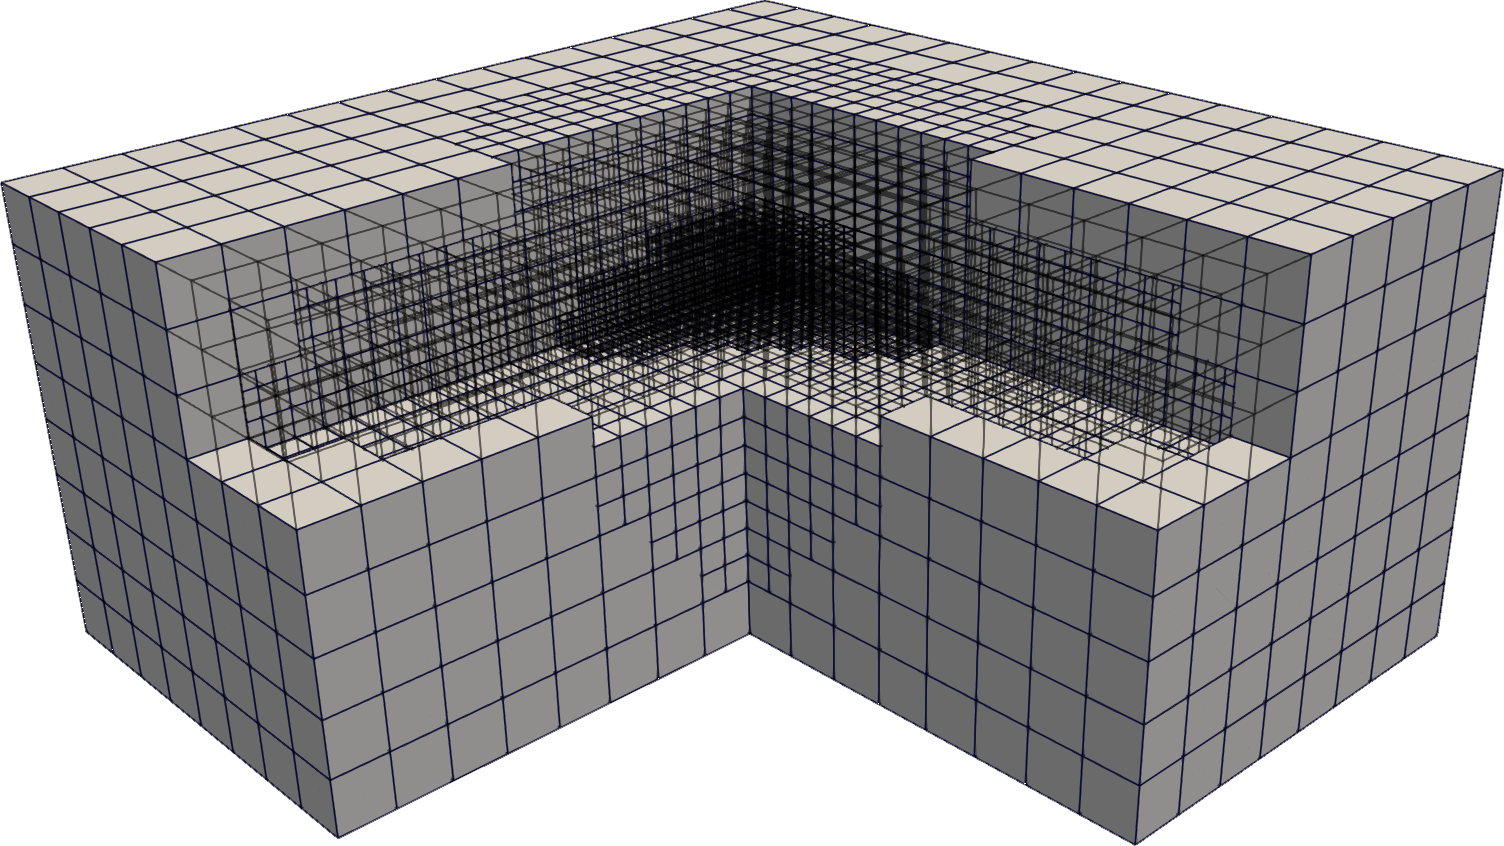
\includegraphics[width=\textwidth]{fichera} % Replace with your own image
    
    \vfill
    
    \Large
    Department of Mathematics\\
    University of Pisa\\
    \today
    
\end{titlepage}


%****************************************************************
% Contents
%****************************************************************

% \maketitle

%\begingroup
%\manualmark
%\setupheading{\contentsname}
\tableofcontents
%\endgroup

%\part{Theory}

% !TeX source = ../main.tex

\chapter[Overview]{Overview}

\section{Notations on Sobolev spaces}
\label{sec:sobolev_notations}

\begin{figure}[!ht]
  \centering
  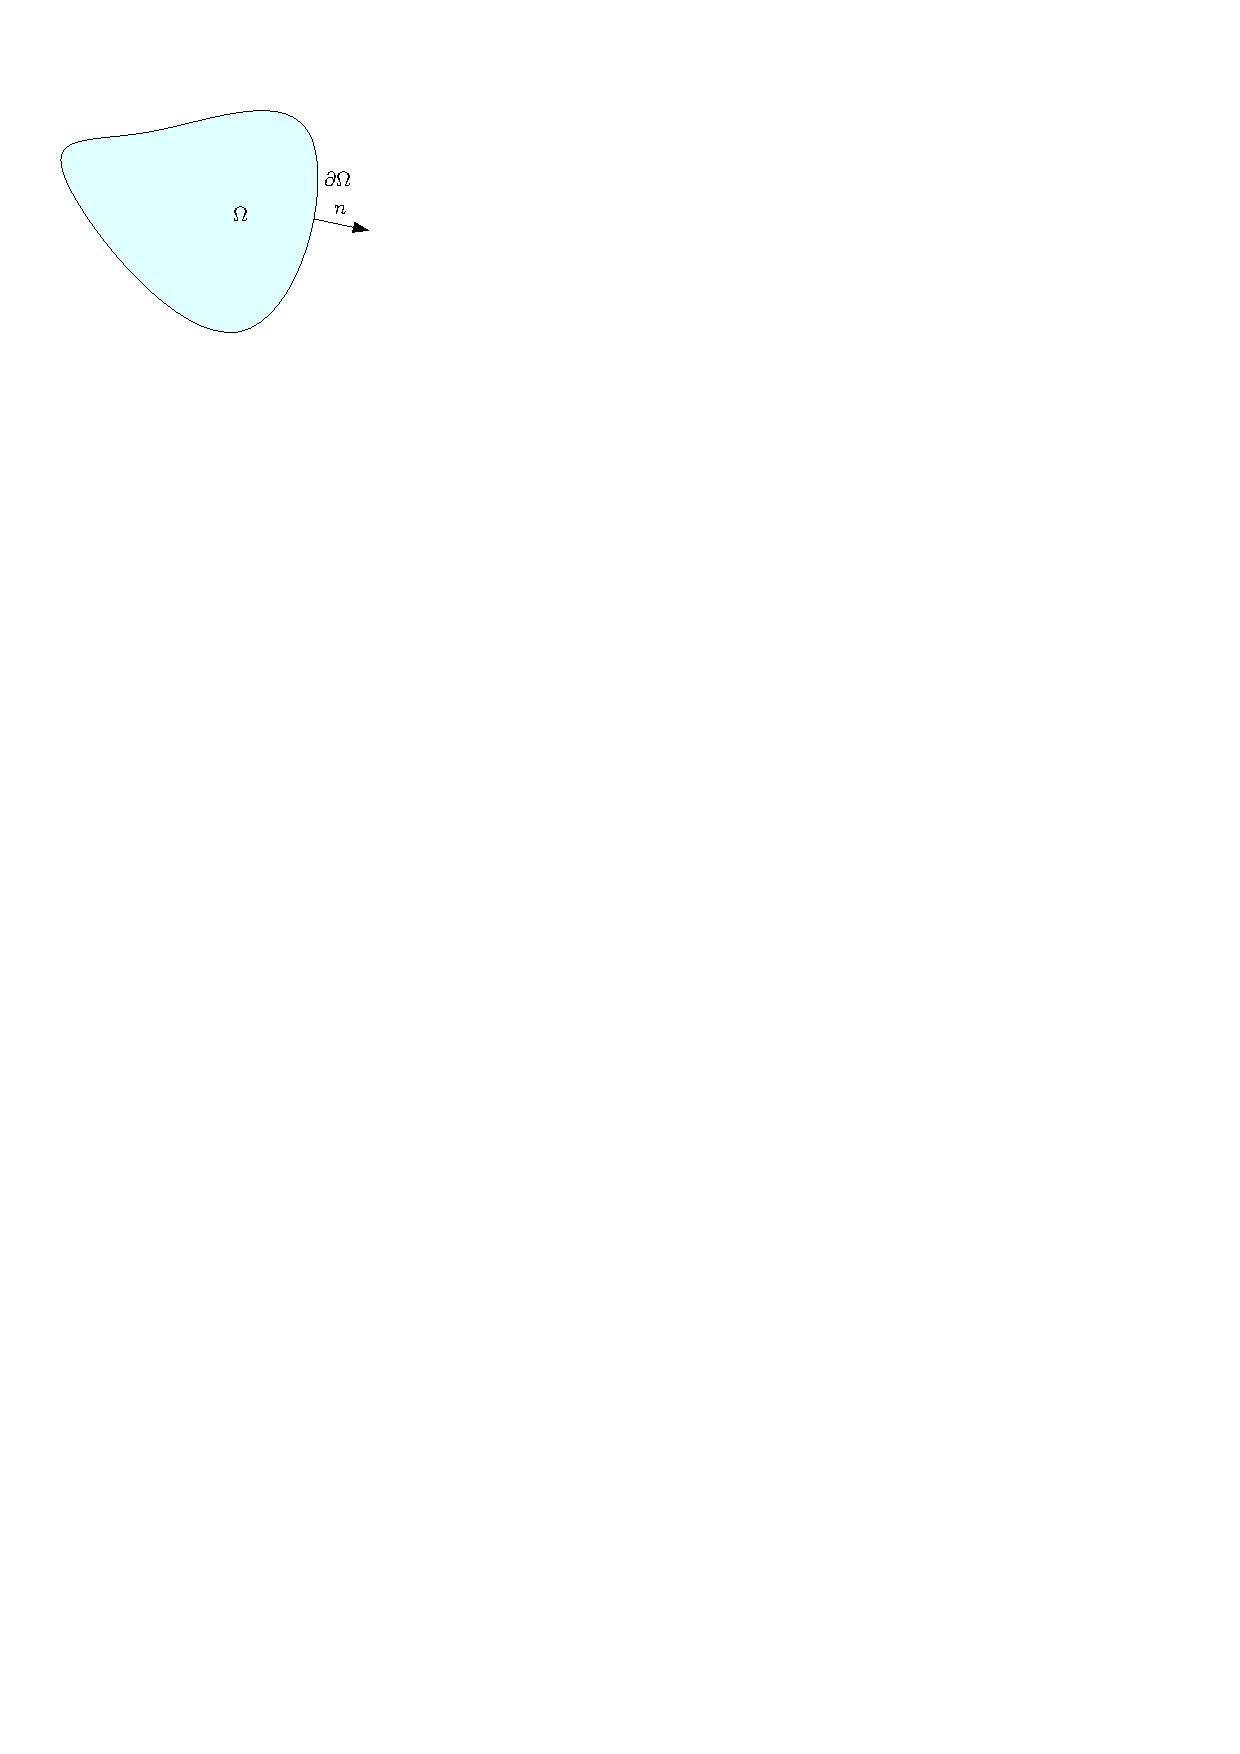
\includegraphics{domain}
  \caption{A Lipschitz domain $\Omega$ and its boundary $\partial\Omega$. We generally indicate with $n$ the outer normal to the boundary.}
  \label{fig:domain}
\end{figure}

Let $\Omega \subset \R^d$ be an open, bounded domain with Lipschitz boundary $\partial\Omega$. We begin by introducing some standard functional spaces that will be used throughout this course.

\subsection{Lebesgue spaces}

For $1 \leq p < \infty$, we define the Lebesgue space $L^p(\Omega)$ as the set of measurable functions $u: \Omega \to \R$ such that
\[
\|u\|_{L^p(\Omega)} := \left(\int_\Omega |u(x)|^p \diff x \right)^{1/p} < \infty.
\]

For $p = \infty$, we define $L^\infty(\Omega)$ as the space of essentially bounded measurable functions with the norm
\[
\|u\|_{L^\infty(\Omega)} := \operatorname{ess\,sup}_{x \in \Omega} |u(x)| < \infty.
\]

Finally we define the space of locally integrable functions as $L^1_{loc}(\Omega)$ where every function $u: \Omega \to \R$ is:
\begin{itemize}
\item measurable;
\item $u|_{K} \in L^1(K)$ for each compact subset $K \subseteq \Omega$.
\end{itemize}

These spaces, equipped with their respective norms, are Banach spaces. In particular, $L^2(\Omega)$ is a Hilbert space with the inner product
\[
(u, v)_{L^2(\Omega)} = \int_\Omega u(x) v(x) \diff x.
\]



\subsection{Weak derivatives}

Let $\alpha = (\alpha_1, \alpha_2, \ldots, \alpha_d)$ be a multi-index with $|\alpha| = \alpha_1 + \alpha_2 + \cdots + \alpha_d$. For a function $u \in C^{|\alpha|}(\Omega)$, we define the standard partial derivative
\[
D^\alpha u = \frac{\partial^{|\alpha|} u}{\partial x_1^{\alpha_1} \partial x_2^{\alpha_2} \cdots \partial x_d^{\alpha_d}}.
\]

For functions that are not sufficiently smooth, we introduce the concept of weak derivatives.

\begin{definition}[Weak derivative]
Let $u \in L^1_{\text{loc}}(\Omega)$ and $\alpha$ be a multi-index. A function $v \in L^1_{\text{loc}}(\Omega)$ is called the $\alpha$-th weak derivative of $u$, denoted by $D^\alpha u = v$, if
\[
  \int_\Omega v(x) \phi(x) \diff x =  (-1)^{|\alpha|} \int_\Omega u(x) D^\alpha \phi(x) \diff x  \quad \forall \phi \in C_0^\infty(\Omega).
\]
\end{definition}

\subsection{Sobolev spaces $W^{k,p}(\Omega)$ and $H^k(\Omega)$}

For integers $k \geq 0$ and $1 \leq p \leq \infty$, we define the Sobolev space $W^{k,p}(\Omega)$ as
\[
W^{k,p}(\Omega) = \{u \in L^p(\Omega) : D^\alpha u \in L^p(\Omega) \text{ for all } |\alpha| \leq k\},
\]
where $D^\alpha u$ are weak derivatives. For $p < \infty$, this space is equipped with the norm
\[
\|u\|_{k,p,\Omega} := \left( \sum_{|\alpha| \leq k} \|D^\alpha u\|_{L^p(\Omega)}^p \right)^{1/p}.
\]

For $p = \infty$, we define
\[
\|u\|_{k,\infty,\Omega} = \max_{|\alpha| \leq k} \|D^\alpha u\|_{L^\infty(\Omega)}.
\]

We also define the seminorm
\[
|u|_{k,p,\Omega} = \left( \sum_{|\alpha| = k} \|D^\alpha u\|_{L^p(\Omega)}^p \right)^{1/p},
\]
with a similar modification for $p = \infty$.

When $p = 2$, we denote $W^{k,2}(\Omega)$ by $H^k(\Omega)$, which is a Hilbert space with the inner product
\[
(u, v)_{H^k(\Omega)} = \sum_{|\alpha| \leq k} (D^\alpha u, D^\alpha v)_{L^2(\Omega)}.
\]

In this case, we simplify the notation for the definition of the norm, and we omit the subscript $2$ (and the domain $\Omega$ if no confusion can arise) for the $H^k$-norm:
\[
  \|u\|_{k} \equiv \|u\|_{k,\Omega} := \|u\|_{k,2,\Omega} = \left( \sum_{|\alpha| \leq k} \|D^\alpha u\|_{L^2}^2 \right)^{1/2}.
\]

\subsection{Sobolev spaces with vanishing boundary values}

For functions in Sobolev spaces, we define the subspace of functions vanishing on the boundary $\partial\Omega$. For $1 \leq p < \infty$, we define
\[
W_0^{k,p}(\Omega) = \overline{C_0^\infty(\Omega)}^{\|\cdot\|_{W^{k,p}(\Omega)}},
\]
that is, the closure of $C_0^\infty(\Omega)$ with respect to the $W^{k,p}$-norm.

In particular, we denote $W_0^{k,2}(\Omega)$ by $H_0^k(\Omega)$. A key property of $H_0^1(\Omega)$ is the Poincaré inequality, which states that there exists a constant $C_{\Omega} > 0$ such that
\[
\|u\|_{L^2(\Omega)} \leq C_{\Omega} \|\nabla u\|_{L^2(\Omega)} \quad \forall u \in H_0^1(\Omega).
\]

This implies that the seminorm $|u|_{H^1(\Omega)} = \|\nabla u\|_{L^2(\Omega)}$ is actually a norm on $H_0^1(\Omega)$ equivalent to the standard $H^1$-norm.

\subsection{Dual spaces}

For a Banach space $X$, we denote by $X'$ its dual space, i.e., the space of continuous linear functionals on $X$. For example, $H^{-1}(\Omega) = (H_0^1(\Omega))'$ denotes the dual of $H_0^1(\Omega)$. We indicate with $\langle \cdot, \cdot \rangle$ the duality pairing between $X$ and $X'$, and we write $f(u) \equiv \langle f, u \rangle$ for $f \in X'$ and $u \in X$.

The norm of a functional $f \in X'$ is defined as
\[
\|f\|_{X'} = \sup_{u \in X} \frac{|\langle f, u \rangle|}{\|u\|_X}.
\]

\subsection{Riesz representation theorem}

For Hilbert spaces, we have a powerful characterization of the dual space through the Riesz representation theorem.

\begin{theorem}[Riesz representation theorem]
  \label{theo:riesz_representation}
Let $H$ be a Hilbert space with inner product $(\cdot, \cdot)_H$. For every bounded linear functional $f \in H'$, there exists a unique element $\tau f \in H$ such that
\[
f(v) = \langle f, v \rangle = (\tau f, v)_H \quad \forall v \in H,
\]
and furthermore,
\[
\|f\|_{H'} = \|\tau f\|_H.
\]
The operator $\tau$ is the so called Riesz operator.
\end{theorem}

This theorem establishes an isometric isomorphism between a Hilbert space and its dual. In particular, for $H = L^2(\Omega)$, given $f \in L^2(\Omega)$, we can identify the functional 
\[
v \mapsto \int_\Omega f v \, \mathrm{d}x
\]
with $f$ itself. Similarly, for $H = H^1_0(\Omega)$, every element in $H'$ can be represented uniquely as an inner product with some element in $H$.

The Riesz representation theorem is especially useful in characterizing the action of operators and in proving existence of solutions to variational problems, as it allows us to convert abstract duality pairings into concrete inner products.

\subsection{Bilinear forms and operators}

Let $X$ and $Y$ be Banach spaces. A bilinear form $a: X \times Y \to \mathbb{R}$ is said to be bounded (or continuous) if there exists a constant $C > 0$ such that
\[
|a(u, v)| \leq C \|u\|_X \|v\|_Y \quad \forall u \in X, \forall v \in Y.
\]

Given a bilinear form $a: X \times Y \to \mathbb{R}$, we can define its associated operator $A: X \to Y'$ by
\[
\langle Au, v \rangle = a(u, v) \quad \forall u \in X, \forall v \in Y,
\]
where $\langle \cdot, \cdot \rangle$ denotes the duality pairing between $Y'$ and $Y$.

The operator $A$ is linear and it inherits the boundedness of $a$, i.e.,
\[ 
  \|A\|_* := \|A\|_{\mathcal{L}(X,Y')} = \sup\limits_{u \in X, v \in Y} \frac{|a(u,v)|}{\|u\|_X \|v\|_Y}.
\]

When $X = Y$ is a Hilbert space, a bilinear form $a: X \times X \to \mathbb{R}$ is said to be:
\begin{itemize}
  \item Symmetric if $a(u, v) = a(v, u)$ for all $u, v \in X$
  \item Coercive (or elliptic) if there exists $\alpha > 0$ such that $a(u, u) \geq \alpha \|u\|_X^2$ for all $u \in X$
\end{itemize}

\subsection{Trace spaces and the trace operator}

For functions in $H^1(\Omega),$ we can define their traces on the boundary $\partial\Omega$. The trace operator 
\[
\gamma: H^1(\Omega) \to H^{1/2}(\partial\Omega)
\]
is a bounded linear operator that extends the classical restriction to the boundary. For simplicity, we often write $u|_{\partial\Omega}$ for $\gamma(u)$.

The space $H^{1/2}(\partial\Omega)$ is a fractional Sobolev space on the boundary, and it can be characterized as the set of traces of $H^1(\Omega)$ functions.

A fundamental result is that $u \in H_0^1(\Omega)$ if and only if $u \in H^1(\Omega)$ and $\gamma(u) = 0$.

\subsection{Sobolev embeddings}

Sobolev spaces embed into other spaces in ways that formalize the intuitive notion that functions with more derivatives tend to be more regular. The Sobolev embedding theorems are crucial tools that allow us to relate Sobolev spaces to classical function spaces.

\begin{theorem}[Sobolev embedding]
Let $\Omega \subset \mathbb{R}^d$ be a bounded domain with Lipschitz boundary, $k \geq 0$ an integer, and $1 \leq p < \infty$. Then:

\begin{enumerate}
  \item If $kp > d$, then the following continuous embedding holds:
  \[
  W^{k,p}(\Omega) \hookrightarrow C^{0}(\overline{\Omega}),
  \]
  i.e., every function in $W^{k,p}(\Omega)$ has a continuous representative.
  
  \item If $s \geq 1$, $p,q \in [1, \infty]$, and 
  \[
  s - \frac{d}{p} > k - \frac{d}{q},
  \]
  then the following continous inclusion holds true:
  \[ 
    W^{s,p}(\Omega) \subset W^{t,q}(\Omega).
  \]
\end{enumerate}
\end{theorem}

The first case is of particular interest when we need our functions to be continuous. The condition $kp > d$ gives us a relationship between:

\begin{itemize}
  \item The order of derivatives $k$
  \item The integrability $p$ of those derivatives
  \item The dimension $d$ of the domain
\end{itemize}

For example, in two dimensions ($d=2$):
\begin{itemize}
  \item $H^2(\Omega) = W^{2,2}(\Omega) \hookrightarrow C^0(\overline{\Omega})$ since $2 \cdot 2 > 2$
  \item $W^{1,p}(\Omega) \hookrightarrow C^0(\overline{\Omega})$ for any $p > 2$
  \item $H^{1}(\Omega) \not\hookrightarrow C^0(\overline{\Omega})$
\end{itemize}

More generally, in $d$ dimensions, we need $k > \frac{d}{p}$ to ensure continuity.

These embedding results are particularly important in numerical analysis, as they help determine when finite element approximations lead to continuous functions. For standard Lagrangian finite elements, the continuity of basis functions is essential, and these embedding theorems provide the theoretical foundation for when such continuity can be expected.

%****************************************************************
% Lezione 27 febbraio
%****************************************************************

\section{Model problem: the Poisson equation}

Let $\Omega$ be an open, bounded, Lipschitz subset of $\R^d$. Let also $\partial\Omega$ be its boundary.
Consider the following Poisson problem:
\[
\begin{cases} \marginpar{Strong formulation}
-\Delta u = f \qquad &\text{in $\Omega$} \\
u =  0 \qquad &\text{on $\partial \Omega$}
\end{cases}
\]
where, as usual,
\[
\Delta = \sum_{i=1}^d \frac{\partial^2}{\partial x_i^2}.
\]
If we want to find a numerical solution for this problem, two approaches can be followed:
\begin{itemize}
\item discretize $-\Delta$ (\emph{finite differences});
\item consider the \emph{weak formulation} of the problem (\emph{finite elements}).
\end{itemize}

Finite differences work well if $\Omega$ is a rectangular or parallelepiped domain (e.g. a square, a cube and so on) and if $f$ is regular enough (e.g. continuous). In applications, however, the domain's boundary may not be nice at all, and $f$ may not even be continuous.
The finite element approach tries to overcome these difficulties, by shifting the problem to finding a good finite dimensional space that approximates the functional space where the exact solution lives.

The advantage, when compared to, e.g., finite differences, is that we don't discretize the differential operator -- which maintains its continuous definition --  but instead we restrict our exploration of candidate solutions to simple spaces (i.e., space of piecewise polynomial functions), for which we can easily compute the action of the differential operator in an exact way.

To make a concrete example, let us consider the Poisson problem, and let's derive its weak formulation.
Let $\phi \in \D$ a test function (usually $\D=C_0^\infty(\Omega)$). We multiply by $\phi$ both sides of the PDE in the strong formulation and then integrate:
\[
\int_\Omega -\Delta u \phi = \int_\Omega f \phi.
\]
If we integrate by parts and use the fact that $\restr{u}{\partial \Omega} = \restr{\phi}{\partial\Omega} = 0$, we get:
\[
\int_\Omega \nabla u \nabla \phi = \int_\Omega f \phi.
\]
More in general, if we replace $\D$ with some appropriate function space $V$, the weak formulation will be: given $f\in V'$, find $u\in V$ such that
\begin{equation} \label{eqn:weak_1} \marginpar{Weak form (1)}
\int_\Omega \nabla u \nabla v = \int_\Omega f v \quad \forall v\in V.
\end{equation}
with the agreement that, being $f \in V'$, the RHS is in fact a duality.

On one side, we need that $\int_\Omega | \nabla u \nabla v | < +\infty$, and on the other side, we need that $u$ and $v$ should be zero on the domain boundary. A natural choice is then the Hilbert space $H^1_0(\Omega)$.

How do we guarantee that a solution to such problem exists? We prove this in an abstract Hilbert setting:
\begin{lemma}[Lax-Milgram]\label{lemma:lax-milgram}\marginpar{Lax-Milgram lemma}
Let $V$ be a Hilbert space and let $a: V\times V \to \R$ be a bilinear operator such that:
\begin{itemize}
\item $a$ is \emph{bounded}, i.e. $\exists c>0$ s.t. 
\[
 a(u,v) \le c \norm{u}_V \norm{v}_V \qquad \forall u,v \in V
 \] 
 (sometimes, we refer to the constant $c$ as $\norm{A}_*$);
\item $a$ is \emph{coercive}, i.e. $\exists \alpha >0$ s.t. 
\[
  a(u,u) \ge \alpha \norm{u}_V^2 \qquad \forall u \in V.
\]
\end{itemize}
Then, given $f\in V'$, the following problem
\begin{equation}\label{eqn:weak_laxmilgram}
a(u,v) = \langle f,v \rangle \quad \forall v\in V
\end{equation}
admits a unique solution $u_0$. Moreover, $u_0$ satisfies the following inequality:
\[
\norm{u_0}_V \le \frac{\norm{f}_{V'}}{\alpha}.
\]
\end{lemma}
\begin{proof}
  Let's consider the linear operator $A: V \to V'$ defined by $A(u) = a(u,\cdot)$.
  Boundedness of $a$ implies that $A$ is a bounded operator, and coercivity implies that 
  \[
    \langle A u, u \rangle = a(u,u) \ge \alpha \norm{u}_V^2 \quad \forall u \in V.
  \]
  
  Let us consider the map $\phi: V \mapsto V$ defined by 
  \[ 
    \phi(v) = v - \rho \tau(A v - f),
  \]
  where $\rho$ is a positive constant to be chosen later, and $\tau$ is the Riesz operator defined in Theorem~\ref{theo:riesz_representation}. By construction, if $u$ is a fixed point of $\phi$, i.e., $u= \phi(u)$, then $u$ necessarily satisfies $A u = f$. Conversely, if $u$ satisfies $Au=f$, then $u$ is also a fixed point of $\phi(u)=u$. 
  
  We want to show that ellipticity is enough to guarantee that there exists a $\rho$ such that $\phi$ is a contraction, i.e., $\exists! ~u$ s.t. $Au=f$.
  
  We have:
  \begin{align*}
    \norm{\phi(u) - \phi(v)}_V^2 & = \norm{u - v - \rho \tau(A(u - v))}_V^2 \\
    & = \norm{u - v}_V^2 - 2 \rho \langle A(u - v), u - v \rangle + \rho^2 \norm{A(u - v)}_{V'}^2 \\
    & \leq \norm{u - v}_V^2 - 2 \rho \alpha \norm{u - v}^2_V + \rho^2 \|A\|^2 \norm{u - v}_V^2 \\
    & \leq  (1 - 2\rho \alpha + \rho^2 \|A\|^2) \norm{u - v}_V^2.
  \end{align*}
  By choosing $\rho$ such that $0<1 - 2\rho \alpha + \rho^2 \|A\|^2 < 1$, (i.e., $\rho<\frac{2\alpha}{\|A\|}$) we have that $\phi$ is a contraction, and by the Banach fixed point theorem, we have that there exists a unique fixed point $u$ of $\phi$, which is the solution of the problem.
  
  Finally, we can estimate the norm of $u$ by the norm of $f$ and the coercivity constant $\alpha$:
  \[
  \alpha \norm{u}_V^2 \leq \langle A u, u \rangle = \langle f, u \rangle \leq \norm{f}_{V'} \norm{u}_V \qquad \Longrightarrow \qquad \norm{u}_V \leq \frac{\norm{f}_{V'}}{\alpha}.
  \]
\end{proof}

In the Poisson problem's case, the bilinear operator is
\[
a(u,v) = \int_\Omega \nabla u \nabla v,
\]
which is clearly bounded and coercive if $V=H_0^1(\Omega)$. In particular, coercivity follows from the Poincaré inequality which implies that the norm in $V$ is equivalent to the $H^1$ seminorm
\[
\abs{u}_{1,2} = \norm{\nabla u}_{L^2}.
\]
Hence, the weak formulation of the Poisson problem admits a unique solution by the Lax-Milgram lemma.

\section{Introduction to finite elements method}

The reason why the finite element method is powerful is that the differential operators stay untouched and, instead, what is to be simplified is \emph{the set in which the solutions live}. We construct a sequence of subspaces $V_h \subset V$ such that $V_h = \Span\{v_i\}_{i=1}^n$, with $n$ depending on $h$. Then we restrict the weak problem to $V_h$, which inherits the norm from $V$: given $f \in V'$, find $u_h \in V_h$ s.t.
\begin{equation} \label{eqn:weak_2} \marginpar{Discrete weak form}
a(u_h,v_h) = \langle f,v_h \rangle \quad \forall v_h\in V_h.
\end{equation}
The element $u_h$ will be our candidate approximate solution. Since $V_h$ is a Hilbert space, and the bilinear operator $a(\cdot, \cdot)$ is coercive in the entire $V$, then also Problem~\eqref{eqn:weak_2} satisfies the hypotheses of Lax-Milgram lemma, and we conclude that there exists a unique solution. For completeness, however, we shall  prove its existence also using Ritz method.

Since $u_h \in V_h$, there exist unique coefficients $\{u^j\}_{j=1}^n$ such that
\[
u_h = \sum_{j} u^j v_j.
\]
The weak problem \ref{eqn:weak_2} then becomes:
\[
a\left(\sum_{j} u^j v_j ,v_h\right) = \langle f,v_h \rangle \quad \forall v_h\in V_h.
\]
In particular, it will suffice for us to check it for a basis of $V_h$:
\[
\sum_{j} a(v_j, v_i)  u^j = \langle v_i,f \rangle \quad \forall i=1,\dots,n.
\]
Here we have rearranged the objects in the brackets and used linearity to make it clearer that this is a matrix identity: if $A$ is the matrix whose entries are $A_{ij}=a(v_j, v_i)$, then we have to solve the linear system
\[
A \mathbf{u} = \mathbf{f}
\]
where $\mathbf{u}=\{u^i\}_{i=1}^n$ and $\mathbf{f}=\{\langle f, v_i\rangle\}_{i=1}^n$.
In particular, $A$ is clearly symmetric and positive definite due to the coercivity of $a$:
\[
\mathbf{u}^T A \mathbf{u} = a(\sum_{i} u^i v_i, \sum_{j} u^j v_j) \ge \alpha \norm{\sum_{i} u^i v_i}^2 \ge 0
\]
and this, by linearity, is zero if and only if every $u^i$ is zero. We conclude that $A$ is non singular, hence $u_h$ exists and is unique.

We now seek a way to control \emph{a priori} the error introduced by the restriction to $V_h$.
\begin{lemma}[Ceà]\marginpar{Ceà's lemma} \label{lemma:cea}
In the setting of the Lax-Milgram lemma, let $u\in V$ be the solution of the weak problem~\eqref{eqn:weak_laxmilgram} and $u_h \in V_h$ a solution of~\eqref{eqn:weak_2}. Then:
\[
\norm{u - u_h} \le \frac{\norm{A}}{\alpha} \inf_{v_h \in V_h} \norm{u - v_h}.
\]
\end{lemma}
\begin{proof}
Observe that, since $u$ solves the weak problem in the whole $V$, then also
\[
a(u,v_h) = \langle f,v_h \rangle \quad \forall v_h\in V_h.
\]
By linearity, it follows that
\[
a(u - u_h,v_h) = 0 \quad \forall v_h\in V_h.
\]
In particular, this is also true if we substitute $v_h$ with $v_h - u_h$, which is still in $V_h$:
\[
a(u - u_h, v_h - u_h) = 0 \quad \forall v_h\in V_h.
\]
This is an orthogonality property of the error. Now we exploit the properties of $a$:
\begin{align}
\alpha \norm{u - u_h}^2 & \le a(u - u_h, u - u_h) \\
& = a(u - u_h, u - v_h) + a(u - u_h, v_h - u_h) \\
& = a(u - u_h, u - v_h) \\
& \le \norm{A} ~\norm {u - u_h} ~ \norm {u - v_h} \quad \forall v_h \in V_h.
\end{align}
The thesis follows by simplifying $\norm{u - u_h}$ on both sides of the inequality, and taking the infimum over $v_h \in V_h$.
\end{proof}

The meaning of Ceà's inequality is: it suffices to control the error only in $V_h$ in order to have a good approximation of $u$. This is a step in the right direction, because in practice the functions in $V_h$ will be piecewise polynomials, hence their derivatives will be well defined and we won't need to approximate them. However, there are still some problems left:
\begin{itemize}
\item How do we approximate an arbitrary domain $\Omega$?
\item How do we approximate $V$ with $V_h$? Meaning, we seek to construct $V_h$ in such a way that $\text{dist}(V,V_h) = c h^k$ for some $k$, where
\[
\text{dist}(V,V_h) = \sup_{u\in V} \inf_{v_h \in V_h} \norm{u - v_h}.
\]
\item In practice, $u$ is unknown, but the RHS of the error estimate contains $u$. How do we manage this?
\end{itemize}



\section{An example: the 1-dimensional case}

\rev{this section could be written better. Polvere note: to me it looks fine, i added a foot note}

Let $\Omega = (a,b)$. In order to discretize it, we consider a set of $n+2$ points $\Set{x_i}_{i=0}^{n+1}$ such that
\[
a = x_0 < x_1 < \dots < x_{n+1} = b.
\]
To keep things simple, let
\[
x_i = a+ih, \quad h = \frac{b-a}{n+1}.
\]
Let $V=H_0^1((a,b))$. Now consider
\[
V_h = \Set{v \in C^0([a,b]): \restr{v}{[x_i, x_{i+1}]}\in \P^1([x_i, x_{i+1}]) \,\forall i=0,\dots,n, \, v(a)=v(b)=0}
\]
where $\P^1$ denotes the space of polynomials of degree at most 1. This space has dimension $n$ and contains piecewise linear functions on $[a,b]$ which are zero on the boundary.

We proceed to find a basis for it: let $v^i(u) := u(x_i)$ the evaluation of $u$ in the node $x_i$, for $i=1,\dots,n$. If $u$ were in $\D$, then $v^i$ would act as a Dirac delta $\delta(x-x_i)$, since
\[
\langle v^i, u \rangle = \int_\Omega \delta(x-x_i) u(x) \diff x = u(x_i).
\]
We construct functions $v_j \in V_h$ such that
\[
v^i(v_j) = \delta_{ij} = \begin{cases}
1 \quad \text{if } i=j \\
0 \quad \text{if } i\ne j
\end{cases}
\quad \forall i,j \in \{1,\dots,n\}.
\]
In practice, for every node $x_j$ in the interior of $[a,b]$ we are considering a piecewise linear function that is one on that node and zero on any other node. It is clear that the functions $\{v_j\}_{j=1}^{n}$\footnote{These functions are also called "Hat functions" for their peculiar hat form.} form a basis for the space $V_h$. These are the so-called \emph{shape functions}. Instead, the $v^i$-s form a basis for $V_h'$ and are called the \emph{nodal basis functions}.

Let us now get back to the Poisson problem. In the 1-dimensional case, the entries of the matrix $A$ are of the form
\[
A_{ij} = \int_a^b v_j'(x) v_i'(x) \diff x.
\]
Since the nodal functions have been constructed in a \emph{localized} way, it is immediate to notice that $A_{ij} = 0$ whenever the supports of the involved nodal functions do not intersect. This is a distinguishing feature of a finite element method: the matrix $A$ is constructed in a way that makes it \emph{sparse}. In particular, in this case we have
\[
A_{ij} = \begin{cases}
0 \quad &\text{if } \abs{i-j}>1 \\
-\frac{1}{h} \quad &\text{if } \abs{i-j}=1 \\
\frac{2}{h} \quad &\text{if } i=j
\end{cases}.
\]
Notice that we have obtained the same matrix we would get with a finite difference method of the same order (with the exception of a scaling factor of $1/h$).

\section{The definition of finite element}

\rev{this section has not been revised yet.}

Let $V$ a Banach space \rev{check if $V$ is only Banach} and $A \in \L(V,V')$ a linear, continuous operator from $V$ to its dual space. Given $f \in V'$, we want to solve the problem $Au=f$ in $V'$, i.e.
\begin{equation}
    \label{eqn:op_pbm} \marginpar{Operator form}
    \langle Au,v \rangle = \langle f,v \rangle \quad \forall v\in V.
\end{equation}
Let $V \supset V_h = \Span\{v_i\}_{i=1}^n$, with $\dim V_h = n$. The space $V_h'$ is usually described in terms of the \emph{covectors}:
\[
V_h' = \Span\{v^i\}_{i=1}^n.
\]
In particular, each $v^i$ is extended via the Hahn-Banach theorem to $V'$, in order to see $V_h'$ as a subspace of $V'$. With this notation, each $v^i$ is the dual vector of $v_i$, i.e.
\[
v^i(v_j) = \delta_{ij}.
\]
\rev{I'm not very sure about this. The $v^i$s are functions in $V'$, but $V_h'$ is not a subspace of $V'$.}
In particular, if $u_h\in V_h$, we have
\[
u_h = \sum_{i=1}^n u^i v_i = \sum_{i=1}^n v^i(u_h) v_i.
\]
This leads to the natural definition of the \emph{interpolation operator} in $V_h$:
\begin{align}
I_{V_h}: &V \to V_h \\
& u \mapsto \sum_{i=1}^n v^i(u) v_i = \sum_{i=1}^n u^i v_i.
\end{align}

\begin{remark}
$I_{V_h}$ is a projection. In fact:
\begin{align}
I_{V_h}(I_{V_h}(u)) &= v^i (u^j  v_j) v_i \\
&= u^j v^i(v_j) v_i \\
&= \delta_{ij} u^j  v_i \\
&= u^i  v_i.
\end{align}
\end{remark}

\begin{definition}[Ciarlet, 1978] \marginpar{Definition of finite element}
A \emph{finite element} is a triplet $(K,P,\Sigma)$, where:
\begin{romanlist}
\item $K\subset \R^n$ is a closed subset with piecewise smooth boundary;
\item $P$ is a finite dimensional space of \emph{shape functions} $v_i$;
\item $\Sigma$ is a set of basis functions $v^i$ for the space $P'$.
\end{romanlist}
\end{definition}


\section{Lagrangian finite elements}

\section{DoFs and finite dimensional spaces}


% !TeX source = ../main.tex

\chapter[A priori error estimates (Lax-Milgram case)]{A priori error estimates (Lax-Milgram case)}

\section{Triangulation of the domain $\Omega$}
In FEM (Finite Element Methods) we discretize the domain $\Omega$ in \emph{simple subdomains} (like triangles for example) where it's easy to define polynomials. Formally speaking we partition $\Omega$
\begin{equation*}
\Omega = \Bigl(\bigcup_{m=1}^M T_m \Bigr)
\end{equation*}
where 
\begin{equation}
T_i \cap T_j = \begin{cases}\emptyset \\ \text{vertex} \\ \text{boundary face}.\end{cases}
\end{equation}
We call this partition \emph{triangulation}. We emphasize that triangulation is just an historical term: we can have triangulations composed of different shapes.

Generally speaking the domain $\Omega$ might be a manifold so it might be needed to have some kind of family of maps (an atlas) that connects a "generic standard" element (we will call it reference triangle) of the triangulation to the true elements of the partitioning of $\Omega$. 

\section{Scaling argument for Sobolev norms}

%%%%%
% Lecture of 20 of March
%%%%%
\begin{figure}[!ht]
\centering
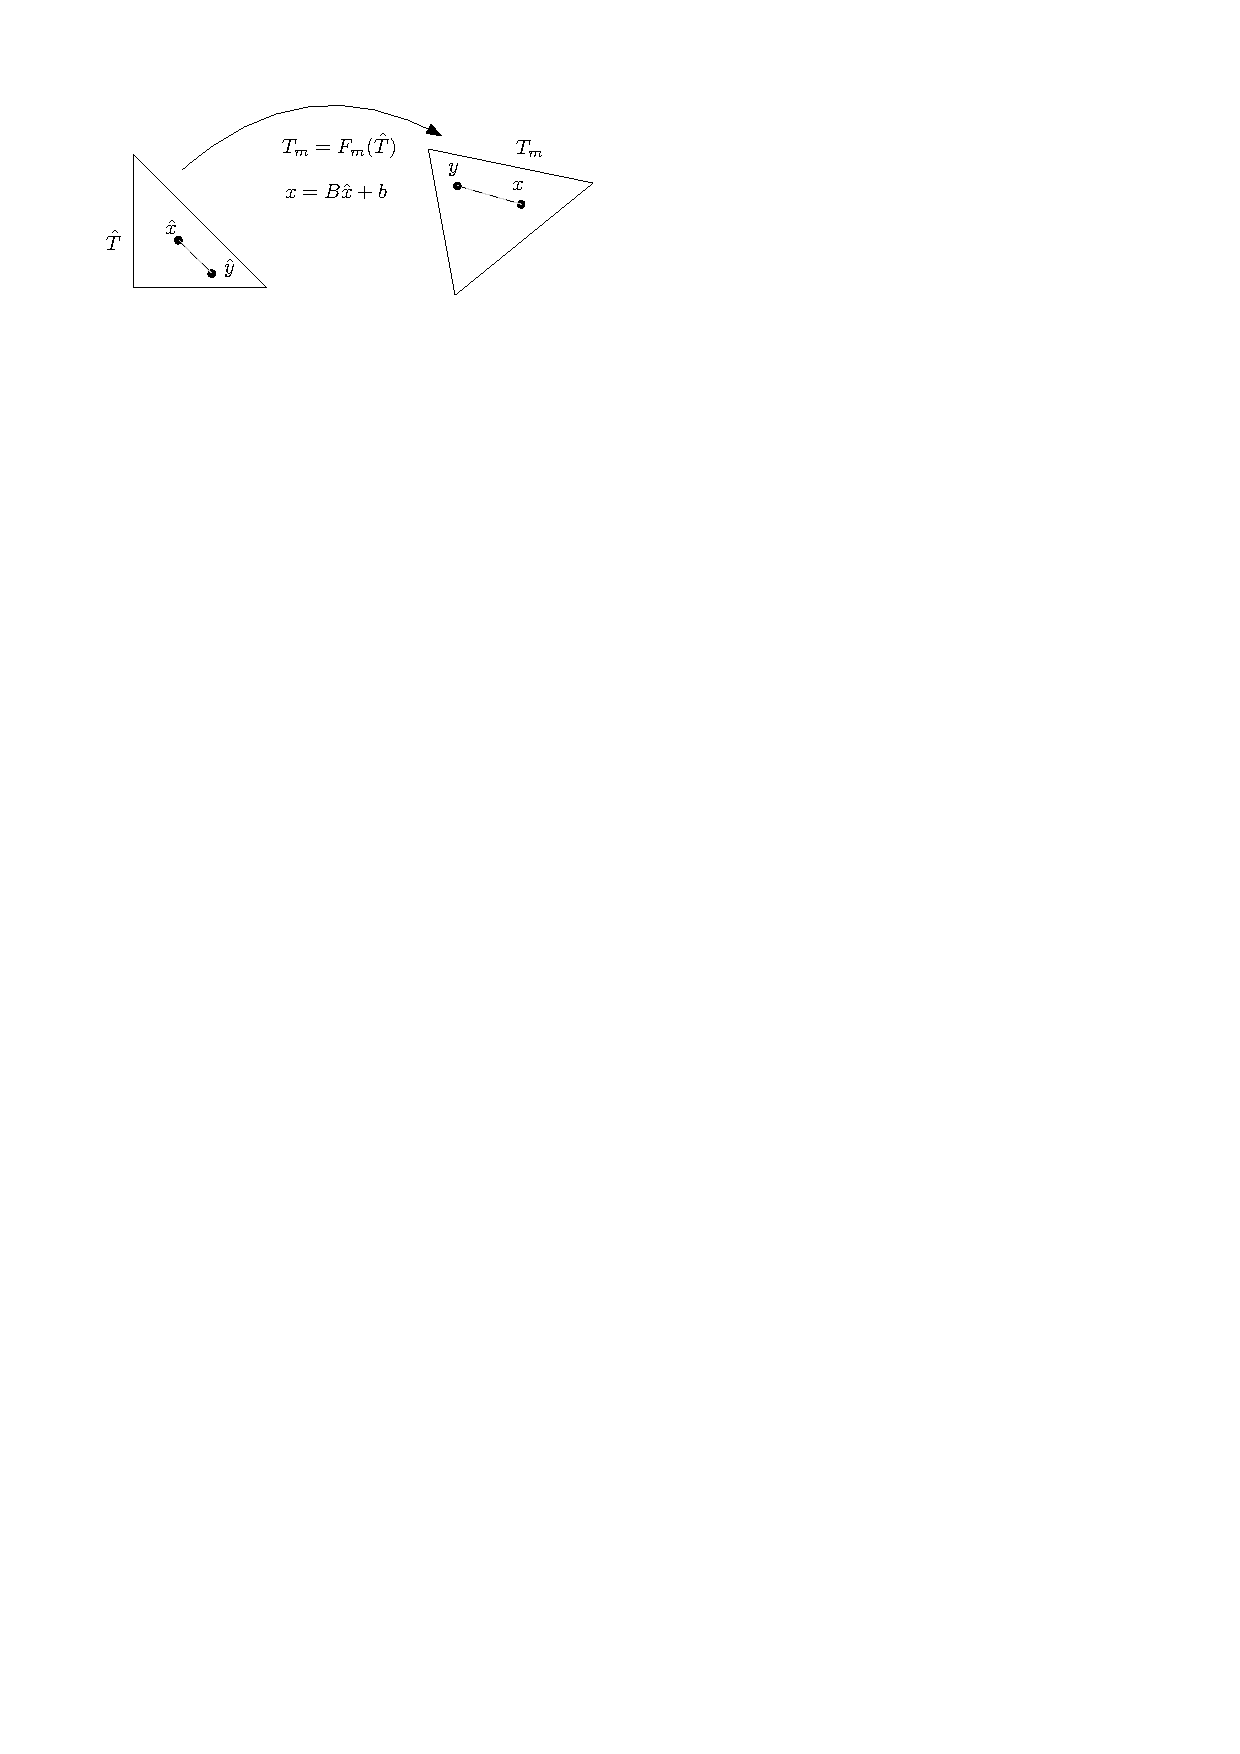
\includegraphics{affine_mapping}
\caption{A triangle $T_m$ and its reference triangle $\hat{T}$. The affine mapping $F_m$ maps $\hat{T}$ to $T_m$.}
\label{fig:affine_mapping}
\end{figure}

Consider an affine mapping from a reference triangle $\hat T$, to a generic triangle $T_m$ (Figure~\ref{fig:affine_mapping}):
\begin{align}
F_m: &\hat{T} \to T_m \\
&\hat{x} \mapsto x = B \hat{x} + b.
\end{align}
We would like to analyze how Sobolev norms change under the action of $F_m$. Recall the the definition of the Sobolev norm in $W^{k,p}$:
\[
\norm{v}^p_{k,p,\Omega} = \sum_{\abs{\alpha} \le k} \norm{D^\alpha v}^p_{L^p(\Omega)},
\]
with the corresponding seminorm:
\[
\abs{v}^p_{k,p,\Omega} = \sum_{\abs{\alpha} = k} \norm{D^\alpha v}^p_{L^p(\Omega)}.
\]

Let
\[
\rho_m := \sup_{\tilde{B} \subset T_m} \diam(\tilde{B}), \quad h_m := \inf_{T_m \subset \tilde{B}} \diam(\tilde{B}),
\]
and similarly for the reference triangle $\hat{T}$:
\[
\hat{\rho} := \sup_{\tilde{B} \subset \hat{T}} \diam(\tilde{B}), \quad \hat{h} := \inf_{\hat{T} \subset \tilde{B}} \diam(\tilde{B}),
\]
where $\tilde{B}$ denotes a ball in the right space (see Figure~\ref{fig:scaling}).


\begin{figure}[!ht]
\centering
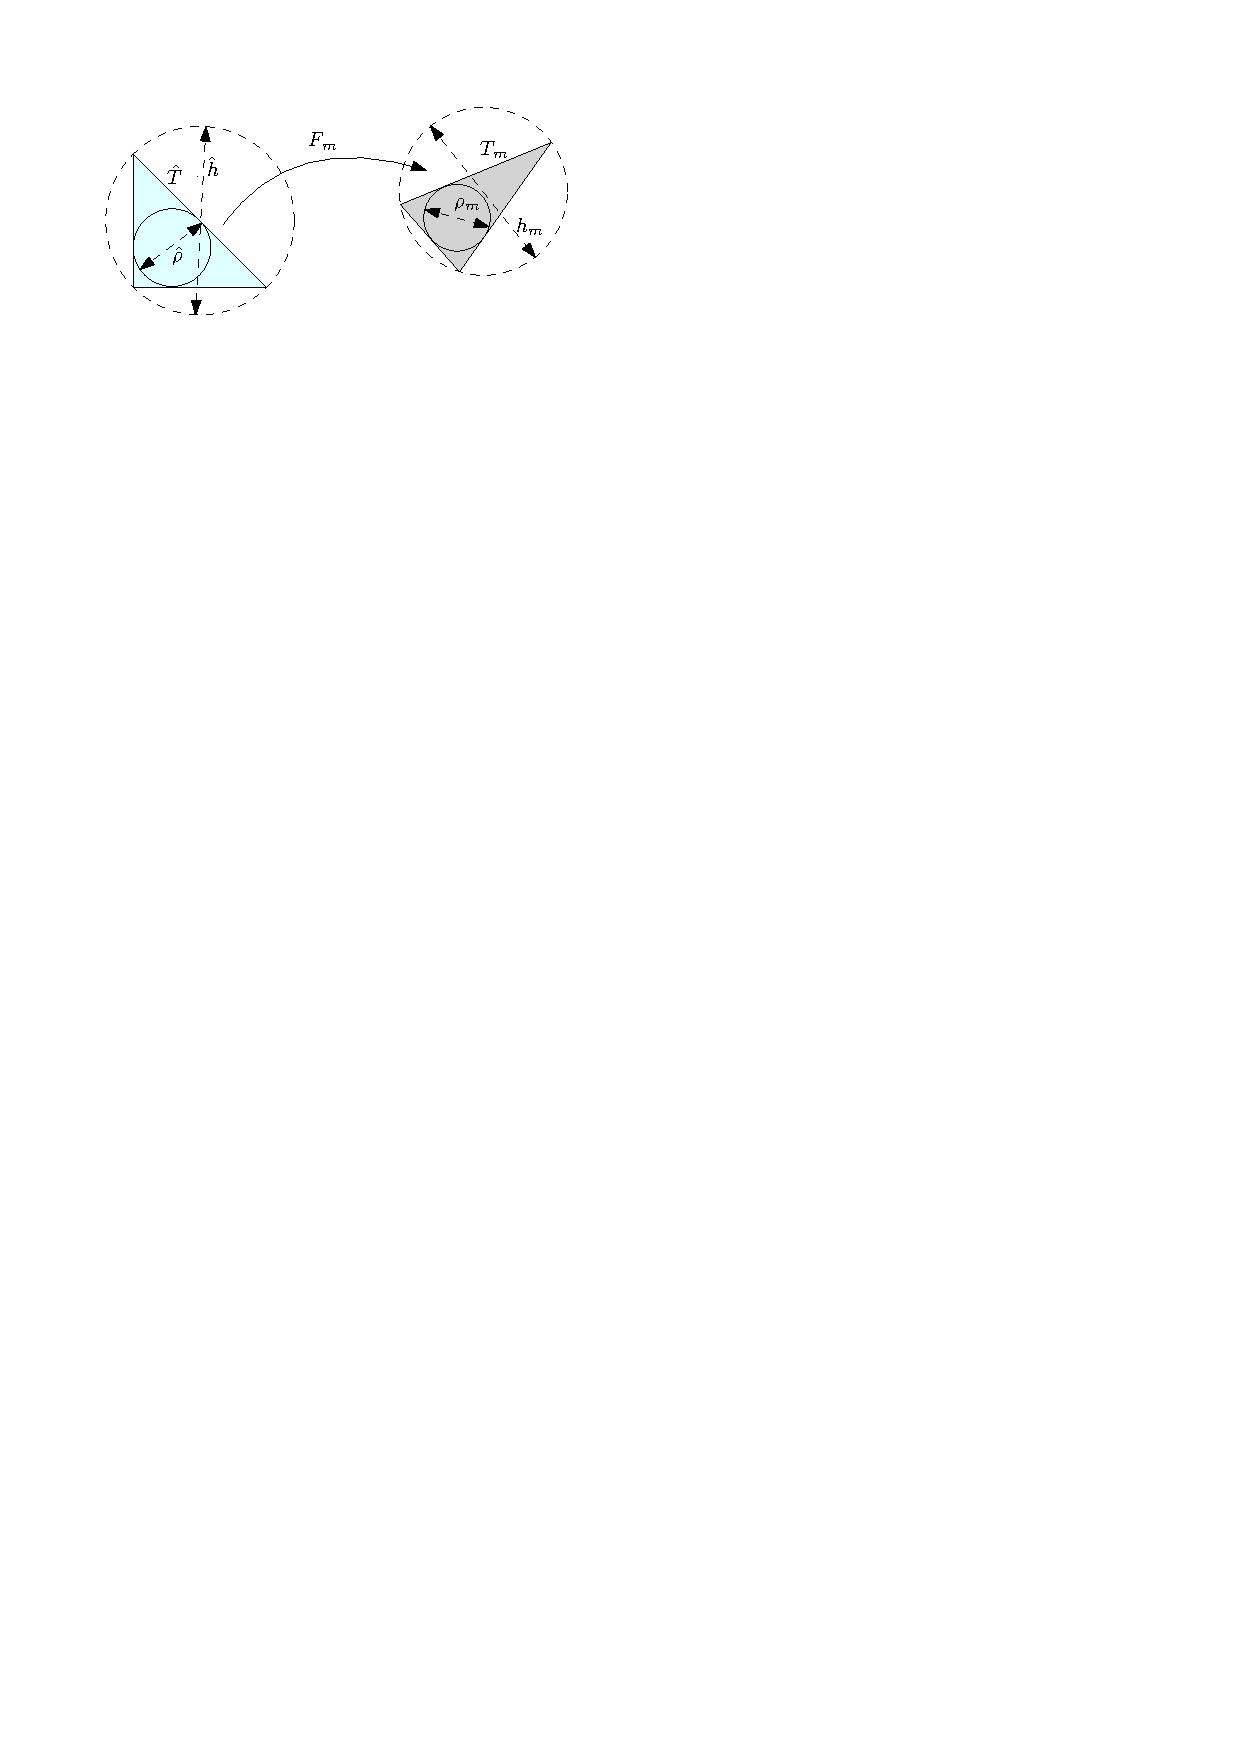
\includegraphics{triangle_scales}
\caption{The scales $\rho_m$ and $h_m$ for a triangle $T_m$, and $\hat \rho$, $\hat h$ for the reference triangle $\hat T$.}
\label{fig:scaling}
\end{figure}


We start with some considerations on the matrix $B$. First, we notice that if $x,y \in T_m$ we have
\[
\abs{x-y} = \abs{B(\hat{x}-\hat{y})} = \abs{B \xi}, \qquad \xi = \hat{x}-\hat{y}.
\]
By the definition of the norm of B, we have that
\begin{equation}
\norm{B} = \sup_{\abs{\xi} = \hat{\rho}} \frac{\abs{B \xi}}{\abs{\xi}} \le
\sup_{\abs{\xi} = \hat{\rho}} \frac{\abs{x-y}}{\hat{\rho}} \le \frac{h_m}{\hat{\rho}}.
\label{eqn:scaling_B}
\end{equation}
With a similar argument:
\begin{equation}
  \norm{B^{-1}} = \sup_{\abs{\xi} = \rho_m} \frac{\abs{B^{-1} \xi}}{\abs{\xi}} \le \frac{\hat{h}}{\rho_m},
  \label{eqn:scaling_B_inv}
\end{equation}
where both $\hat \rho$ and $\hat h$ are constant, and depend only on the choice of the reference triangle $\hat T$.
Also, since $F_m$ is affine, its differential is the matrix $B$ itself. This will come in handy to provide a simple formula for $\hat{D}^\alpha (v \circ F_m)$ when using the chain rule.

Consider a function $v \in W^{k,p}(T_m)$ on the triangle $T_m$. Then:
\begin{align}
\abs{v \circ F_m}^p_{k,p,\hat{T}} 
&= \sum_{\abs{\alpha} = k} \int_{\hat{T}} \abs{ \hat{D}^\alpha (v \circ F_m)}^p \diff\hat{T} \\
&= \sum_{\abs{\alpha} = k} \int_{\hat{T}} \abs{ [(D^\alpha v) \circ F_m)] B^{\abs{\alpha}}}^p \diff\hat{T} \\
&= \sum_{\abs{\alpha} = k} \int_{\hat{T}} \abs{ [(D^\alpha v) \circ F_m)] B^{\abs{\alpha}}}^p J^{-1} J \diff\hat{T} \\
&= \sum_{\abs{\alpha} = k} \int_{T} \abs{ D^\alpha v B^{\abs{\alpha}}}^p J^{-1} \diff T \\
&\le \norm{B}^{kp} J^{-1} \sum_{\abs{\alpha} = k} \int_{T} \abs{ D^\alpha v}^p \diff T,
\end{align}
where $J$ is the absolute value of the Jacobian of the transformation $F_m$ (in the present case, $J=\abs{\det B}$). Hence, using~\eqref{eqn:scaling_B}, we conclude:
\[
\abs{v \circ F_m}_{k,p,\hat{T}} \le \norm{B}^k J^{-\frac{1}{p}} \abs{v}_{k,p,T}
\le c h_m^k J^{-\frac{1}{p}} \abs{v}_{k,p,T},
\]
and similarly, using~\eqref{eqn:scaling_B_inv}:
\[
\abs{v}_{k,p,T} \le \norm{B^{-1}}^k J^{\frac{1}{p}} \abs{v \circ F_m}_{k,p,\hat{T}}
\le c \rho_m^{-k} J^{\frac{1}{p}} \abs{v \circ F_m}_{k,p,\hat{T}},
\]
where $c$ is a constant depending on the reference triangle $\hat{T}$, but not on the triangle $T_m$.

For $h_m \le 1$, we can write similar scaling arguments for the full norms:
\begin{align}
    \norm{v \circ F_m}_{k,p,\hat{T}} & \le c h_m^k J^{-\frac{1}{p}} \norm{v}_{k,p,T},\\
    \norm{v}_{k,p,T} & \le c \rho_m^{-k} J^{\frac{1}{p}} \norm{v \circ F_m}_{k,p,\hat{T}}.
\end{align}

From now on we adopt this notation:
\begin{itemize}
\item $a \lesssim b$ means "$\exists c \text{ s.t. } a \le cb$";
\item $a \gtrsim b$ means "$\exists c \text{ s.t. } ca \ge b$";
\item $a \sim b$ means "$a \lesssim b \wedge b \lesssim a$".
\end{itemize}
For example, if two norms $\norm{\cdot}_X$ and $\norm{\cdot}_Y$ are equivalent, the following statements share the same meaning:
\[
\norm{a}_X \sim \norm{a}_Y \iff \exists c,C \text{ s.t. } c\norm{a}_X \le \norm{a}_Y \le C \norm{a}_X.
\]


\section{The Bramble-Hilbert lemma}

\begin{lemma}[Bramble-Hilbert]
Let $V$, $W$, $Q$ be Banach spaces and let $\tau \in \L(V,W)$ be an operator such that $Q \subset \ker(\tau)$. Then:
\begin{enumerate}
\item $\norm{\tau(u)}_W \le \norm{\tau}_* \inf_{q \in Q} \norm{u-q}_V \quad \forall u\in V$.
\item Choosing $V=W^{k+1,p}(\Omega)$, $W=W^{s,p}(\Omega)$, $Q=\P^k(\Omega)$, with $\Omega$ open connected (and bounded Lipschitz) and $0\le s \le k$, we get
\[
\norm{\tau(u)}_{s,p,\Omega} \lesssim \norm{\tau}_* \abs{u}_{k+1,p,\Omega} \quad \forall u\in W^{k+1,p}(\Omega).
\]
\end{enumerate}
\label{lemma:bramble-hilbert}
\end{lemma}

\begin{proof}
The first inequality follows immediately by observing that $\tau$ is linear and that $q\in \ker(\tau)$ implies $\tau(u+q) = \tau(u) + \tau(q) = \tau(u)$, hence:
\[
\tau(u) = \tau(u+q) = \le \norm{\tau}_* \norm{u+q} \qquad \forall q \in Q.
\]

The second inequality follow from the first one by showing that~\cite{ciarlet78}
\begin{lemma}[Denis-Lions]
  \begin{equation}
    \abs{u}_{k+1,p,\Omega} \sim \inf_{q \in \P^k} \norm{u+q}_{k+1,p,\Omega} \qquad \forall u \in W^{k+1,p}(\Omega).
    \label{eqn:deny-lions}
  \end{equation}
\end{lemma}

From now on, we'll omit $\Omega$ for simplicity where its presence is obvious.
\begin{itemize}
\item The inequality $\abs{u}_{k+1,p} \lesssim \inf_{q \in \P^k} \norm{u+q}_{k+1,p}$ is trivial, because every polynomial of degree at most $k$ has zero derivatives of $(k+1)$-th order. Hence
\[
\abs{u}_{k+1,p} = \abs{u+q}_{k+1,p} \le \norm{u+q}_{k+1,p} \quad \forall q \in \P^k.
\]
\item In order to prove that the converse holds, let $\{v_i\}_{i=0}^N$ be a basis for $\P^k$. Then, with the usual notation, $(\P^k)'=\Span\{v^i\}_{i=0}^N$, where the $v^i$-s are such that $v^i(v_j)=\delta_{ij}$. Since $\P^k \subset W^{k+1,p}$, by the Hahn-Banach theorem we can naturally extend these $v^i$-s to be elements of $(W^{k+1,p})'$. Hence we can consider the projection
\begin{align}
\Pi^k:  W^{k+1,p}(\Omega) & \to \P^k(\Omega)\\
u & \mapsto \sum_{i=0}^N v^i(u) v_i.
\end{align}
The key part is proving that
\begin{equation}\label{eqn:deny-lions-exp}
\norm{u}_{k+1,p}^p \sim \abs{u}_{k+1,p}^p + \sum_{i=0}^N \abs{v^i(u)}^p \quad \forall u \in W^{k+1,p}.
\end{equation}
In fact, the $\gtrsim$ inequality follows from bounding the Sobolev seminorm with the corresponding norm and by the simple inequality
\[
\abs{v^i(u)} \le \norm{v^i}_{(W^{k+1,p})'} \norm{u}_{k+1,p}.
\]
The $\lesssim$ inequality, instead, can be proven by contradiction. If it were not true, then for every constant $c$ there would exist $w_c \in W^{k+1,p}$ such that $\norm{w_c}_{k+1,p} = 1$ and
\[
c(\abs{w_c}_{k+1,p}^p + \sum_{i=0}^N \abs{v^i(w_c)}^p) < \norm{w_c}_{k+1,p}^p = c.
\]
If we choose $c=j$ in $[1,2,\dots)$, we obtain a sequence $\{w_j\}$ such that
\begin{equation} \label{eqn:deny-lions-proof}
\abs{w_j}_{k+1,p}^p + \sum_{i=0}^N \abs{v^i(w_j)}^p < \frac{1}{j} \quad \forall j.
\end{equation}
Now, thanks to the compact embedding $W^{k+1,p} \hookrightarrow W^{k,p}$, we have, up to a subsequence, that $w_j \to w$ strongly in $W^{k,p}$ for some $w \in W^{k,p}$.

However, we can easily show that the function $w$ belongs also to $W^{k+1,p}$. In fact, from~\eqref{eqn:deny-lions-proof} we deduce
\[
\abs{w_j}_{k+1,p}^p < \frac{1}{j} \quad \forall j.
\]
This implies that the sequence $\{w_j\}$ is Cauchy also in $W^{k+1,p}$, because
\[
\norm{w_i-w_j}_{k+1,p}^p = \norm{w_i-w_j}_{k,p}^p + \abs{w_i-w_j}_{k+1,p}^p.
\]
Hence, by uniqueness of the limit, $w \in W^{k+1,p}$. Then, by (strong) continuity of the norm, we obtain $\norm{w}_{k+1,p}=1$ and we can pass to the limit the inequality~\eqref{eqn:deny-lions-proof} to get:
\[
\abs{w}_{k+1,p}^p = 0, \quad \sum_{i=0}^N \abs{v^i(w)}^p = 0.
\]
The first equality, since $\Omega$ is an open connected domain, implies that $w \in \P^k(\Omega)$. The second equality implies that $\Pi^k(w)=0$. But for a polynomial in $\P^k$ we have $\Pi^k(w)=w$, hence $w=0$, which is in contradiction with $\norm{w}_{k+1,p}=1$.

We can now conclude, exploiting inequality~\eqref{eqn:deny-lions-exp}, by noticing that
\begin{align}
\inf_{q \in \P^k} \norm{u+q}_{k+1,p} &\le \norm{u- \Pi^k(u)}_{k+1,p} \\
& \lesssim \abs{u-\Pi^k(u)}_{k+1,p}^p + \sum_{i=0}^N \abs{v^i(u-\Pi^k(u))}^p \\
& = \abs{u}_{k+1,p}^p.
\end{align}
where the last equality holds because the summation term is equal to zero by linearity of the $v^i$-s and the seminorm is simplified due to $\Pi^k(u)$ being a polynomial in $\P^k$.
\end{itemize}
\end{proof}

Bramble-Hilbert lemma allows us to provide a-priori error estimates for a finite element method, by quantifying the constants in the inequality throught the scaling arguments presented in the previous section. Consider an affine mapping $F_T: \hat{T} \to T$ and its related quantities $h_T$ and $\rho_T$. 

We can use Bramble-Hilbert lemma applied to the operator $(I-\Pi^k)\circ F_T$ to control the $s$-Sobolev norm of the error $u - \Pi^k(u)$. By repeating the scaling arguments on both $\norm{(u- \Pi^k(u)) \circ F_T}_{s,p,\hat{T}}$ and $\abs{u \circ F_T }_{k+1,p,\hat{T}}$, we get, for any triangle $T = F_T(\hat{T})$:
\begin{align}
\norm{u- \Pi^k(u)}_{s,p,T} &\lesssim \rho_T^{-s} J^{\frac{1}{p}} \norm{(u- \Pi^k(u)) \circ F_T}_{s,p,\hat{T}} \\
& = \rho_T^{-s} J^{\frac{1}{p}} \norm{u \circ F_T - \Pi^k(u) \circ F_T}_{s,p,\hat{T}} \\
& \lesssim \rho_T^{-s} J^{\frac{1}{p}} \abs{u \circ F_T }_{k+1,p,\hat{T}} \\
& \lesssim h_T^{k+1} \rho_T^{-s} \abs{u}_{k+1,p,T} \quad \forall 0\le s \le k.
\end{align}

Overall, we can control the $s$-Sobolev norm of the error up to order $k$ with the Sobolev semi-norm of order $k+1$ of the solution $u$.

If we sum over the cells of the triangulation, we obtain a global \emph{a-priori} inequality:
\[
\sum_{T \in \T_h} \norm{u- \Pi^k(u)}_{s,p,T}^p \lesssim
\sum_{T \in \T_h} \bigl( h_T^{k+1} \rho_T^{-s} \abs{u}_{k+1,p,T} \bigr)^p.
\]
If we let
\[
h = \max_{T \in \T_h} h_T, \quad \rho = \min_{T \in \T_h} \rho_T, \quad \Omega = \mathring{\overline{\bigcup_{T \in \T_h} T}}
\]
then we can bound the RHS of the inequality in this way:
\[
\Bigl( \sum_{T \in \T_h} \norm{u- \Pi^k(u)}_{s,p,T}^p \Bigr)^\frac{1}{p} \lesssim
h^{k+1} \rho^{-s} \abs{u}_{k+1,p,\Omega}.
\]
The LHS is also called a \emph{broken Sobolev norm}, since it is defined element-wise. It is not automatically equal to $\norm{u- \Pi^k(u)}_{s,p,\Omega}$: in order to be, the global space $V_h$, obtained by gluing together the local spaces $P^k(T_m)$, must be \emph{conforming} to $V$. 

\begin{remark}[Conformity] For a finite element space to be conforming, we need to guarantee that the resulting finite dimensional space $V_h$ is indeed included in $V$. While locally every polynomial space $P^k(T)$ is always contained in every Sobolev space $W^{k,p}(T)$ (since $P^k(T) \subset C^{\infty}(T)$ for any $k$), the same cannot be said for the \emph{union} of the local spaces $P^k(T_m)$. Such a space is in general discontinuous (i.e., there is no reason to expect that the polynomials in $P^k(T_m)$ and $P^k(T_n)$ agree on the common face between the two cells $T_m$ and $T_n$), and although continuity is in general not required for Sobolev spaces $W^{k,p}(\Omega)$ (i.e., $W^{k,p}(\Omega)\not\subset C^0(\Omega)$ for $kp\leq d$), one can show that if $k \geq 1/p$, then a discontinuity along a surface of co-dimension one is not allowed.

If we want the finite dimensional space $V_h$ to be conforming with $W^{k,p}(\Omega)$ (for example), then we need to restrict the polynomial spaces on the elements $T_m$ and $T_n$ so that $P^k(T_m)$ and $P^k(T_n)$ agree on the common face between the two cells $T_m$ and $T_n$ for all derivatives up to the degree $k-1$.
\end{remark}

\begin{remark}
The same inequality can be proven if the triangulation $\T_h$ is made of quadrilaterals, and if the mapping is bi-linear instead of affine. In this case, the constants that appear in the error estimates are generally better, and this is why meshes made of quadrilaterals and hexahedra are usually preferred (when available): they are more difficult to construct, but they offer better approximation properties.
\end{remark}

Finally, we can put togetner Ceà's lemma~\ref{lemma:cea} with Bramble-Hilbert lemma~\ref{lemma:bramble-hilbert} to get the following \emph{a priori} error estimate for finite element methods: provided that $A$ is bounded and coercive in $H^s(\Omega)$, for a conforming approximation $V_h \subset V \equiv H^s(\Omega)$ space we have that, if the exact solution is regular enough, i.e. $u \in H^{k+1}(\Omega)$, then
\begin{align} \label{ineq:cea_scaling}
\norm{u - u_h}_{s,\Omega} &\le \frac{\norm{A}}{\alpha} \inf_{v_h \in V_h} \norm{u - v_h}_{s,\Omega} \\
& \le \frac{\norm{A}}{\alpha} \norm{u - \Pi^k(u)}_{s,\Omega} \\
& \lesssim \frac{\norm{A}}{\alpha} \rho^{-s} h^{k+1} \abs{u}_{k+1,\Omega} \quad \forall 0\le s \le k.
\end{align}
The inequality hints at some strategies for error reduction:
\begin{itemize}
\item take $h$ smaller, i.e. \emph{refine the mesh};
\item take $k$ bigger (if possible), which implies increasing the polynomial degree.
\end{itemize}
\begin{remark}[Regularity] In order use the \emph{a-priori} estimate, we need to make sure that the solution $u$ is indeed in the space $H^{k+1}(\Omega)$. This, in general, will depend on $A$, on $f$ and on the regularity of the domain $\Omega$, and it is what the theory of regularity for PDEs attempts to do. In particular, in the following section we will mention the concept of $r$-regularity.
\end{remark}

%%%%%
% Lecture of 27 of March
%%%%%


\section{\texorpdfstring{$H^k$}{Hk} error estimates, Nitsche's lemma}
Consider a triangulation $\T_h$ and recall the quantities $h$ and $\rho$ we defined in the previous section:
\[
h := \max_{T \in \T_h} h_T, \quad \rho := \min_{T \in \T_h} \rho_T.
\]
We say that the mesh is \emph{quasi-uniform} if
\[
\exists \sigma > 0 \text{ s.t. } \rho_T \ge \sigma h_T  \quad \forall T\in \T_h.
\]
For such a mesh, the inequality~\eqref{ineq:cea_scaling} becomes:
\begin{equation} \label{ineq:cea_scaling2}
\norm{u - u_h}_{s,p,\Omega}
\lesssim \frac{\norm{A}}{\alpha} h^{k+1-s} \abs{u}_{k+1,p,\Omega} \quad \forall 0\le s \le k.
\end{equation}
From now on we consider $p=2$ and use the notation $\norm{u}_k$ to mean $\norm{u}_{k,2,\Omega}$.
\begin{definition}
Let $V \subset H^k$ and $A \in \L(V,V')$. We say that $A$ is $r$-\emph{regular} if there exists an interval $[s_{min}, s_{max}]$ such that $\forall g \in H^s$, with $s \in [s_{min}, s_{max}]$, the problem $Au=f$ admits a unique solution $u$ which satisfies
\[
\norm{u}_{s+r} \lesssim \norm{f}_s.
\]
\end{definition}
\rev{Check if on the LHS there is norm or seminorm of $u$.}
The inequality~\eqref{ineq:cea_scaling2}, combined with the assumption of $r$-regularity, becomes
\begin{equation}\label{ineq:cea_scaling3}
\norm{u-u_h}_k \lesssim h^{s+r-k} \abs{u}_{s+r} \lesssim h^{s+r-k} \norm{f}_s \quad \forall 0\le k \le s+r-1.
\end{equation}
This is finally the error estimate we were looking for. However, as said before, we may not be allowed to use all the values for $k$ in the range above, as the following example will show.
\begin{example}
The Poisson problem on a Lipschitz, convex domain is $2$-regular, with $s \le 0$. Hence, the inequality~\eqref{ineq:cea_scaling3} becomes
\[
\norm{u-u_h}_k \lesssim h^{s+2-k} \norm{f}_s \quad \forall 0\le k \le s+1.
\]
In particular, if $k=1$, we get
\[
\norm{u-u_h}_1 \lesssim h^{s+1} \norm{f}_s.
\]
This means that, for instance, if $f \in L^2$, i.e. $s=0$, the order of convergence in the $H^1$ norm is $1$. If $\Omega$ is better than Lipschitz, then the range for $s$ becomes better, hence we gain a better convergence of the numerical approximation (provided that $f$ is more regular).
Unfortunately, we cannot use the $L^2$ norm in Ceà's lemma, and this means that we cannot get an estimate in the $L^2$ norm.
\end{example}

With some bit of additional work, we can produce error estimates on weaker norms, such as the $L^2$ one, from the estimates on stronger norms.
\begin{lemma}[Nitsche] \label{lemma:nitsche}
Let $A \in \L(V,V')$ an operator as in the hypotheses of Lax-Milgram's lemma. Assume that $V$ is a subspace of some Hilbert space $H$, with the following properties:
\begin{romanlist}
\item $\norm{u}_H \lesssim \norm{u}_V$ $\quad \forall u \in V$ \quad (i.e., the embedding $V \hookrightarrow H$ is continuous);
\item $V = \overline{H}^{\norm{\cdot}_V}$.
\end{romanlist}
Then the following inequality holds:
\begin{equation}\label{eqn:nitsche_lemma}
\norm{u-u_h}_H \lesssim \sup_{g \in H} \Bigl( \frac{1}{\norm{g}_H} \inf_{\phi_h \in V_h} \norm{\phi_g - \phi_h}_V \Bigr) \norm{u-u_h}_V .
\end{equation}
\end{lemma}

\begin{remark}
With the hypotheses above, if $f \in H$, by the Hahn-Banach theorem $f$ can be extended to a functional $\tilde{f} \in V'$, i.e.
\[
\langle \tilde{f}, v \rangle_V = (f, v)_H \quad \forall v \in V.
\]
\rev{Is Hahn-Banach really necessary? We are in a Hilbert space setting.}
Now consider the usual problem in operator form $A u = \tilde{f}$, i.e.
\begin{equation}
\langle Au,v \rangle = \langle \tilde{f},v \rangle = (f, v)_H \quad \forall v\in V.
\end{equation}
By the Lax-Milgram lemma, we know that this problem has a unique solution $u \in V$.

With the same philosophy, let $g \in H$ and consider the \emph{dual problem} $A^T \phi = g$, i.e.
\begin{equation}
\langle Av,\phi \rangle = \langle \tilde{g},v \rangle = (g, v)_H \quad \forall v\in V.
\end{equation}
Since also $A^T$ satisfies the hypotheses of the Lax-Milgram lemma, the adjoint problem admits itself a unique solution $\phi_g \in V$.
\end{remark}

\begin{proof}
We start observing that
\begin{equation}\label{eqn:nitsche_norm}
\norm{u-u_h}_H = \sup_{g \in H} \frac{(g, u-u_h)_H}{\norm{g}_H}.
\end{equation}
This is true because $H$ is a Hilbert space, hence $H \cong H'$.

Given $g \in H$, we know from the last remark that the dual problem $A^T \phi = g$ admits a unique solution $\phi_g \in V$. If we set $v = u-u_h$, we get:
\[
\langle A (u-u_h),\phi_g \rangle = (g, u-u_h)_H.
\]
Now we take advantage of the Galerkin orthogonality, i.e. $\langle A (u-u_h), \phi_h \rangle = 0$ $\forall \phi_h \in V_h$:
\[
(g, u-u_h)_H = \langle A (u-u_h),\phi_g - \phi_h \rangle \quad \forall \phi_h \in V_h.
\]
Now we use the continuity of $A$ on~\eqref{eqn:nitsche_norm} to produce the desired estimate:
\begin{align}
\norm{u-u_h}_H &= \sup_{g \in H} \frac{(g, u-u_h)_H}{\norm{g}_H} \\
& = \sup_{g \in H} \frac{\langle A (u-u_h),\phi_g - \phi_h \rangle}{\norm{g}_H} \\
& \le \norm{A} \sup_{g \in H} \Bigl( \frac{1}{\norm{g}_H} \inf_{\phi_h \in V_h} \norm{\phi_g - \phi_h}_V \Bigr)
\norm{u-u_h}_V .
\end{align}
\end{proof}

In practice, we want to use this lemma with $V \subset H^k$ and $H \subset H^s$, with $0\le s < k$, or at least we want that $\norm{\cdot}_V \sim \norm{\cdot}_k$ and $\norm{\cdot}_H \sim \norm{\cdot}_s$. For instance, think as $V=H^1$, $H=L^2$.
\rev{Fix inconsistencies between $\Pi^k$ and $I_h$.}
In order to find a relation between $\norm{\phi_g - \phi_h}_k$ and $\norm{g}_s$, we use the Bramble-Hilbert lemma and the scaling argument, plus the $r$-regularity, but for $A^T$:
\begin{align}
\inf_{\phi_h \in V_h} \norm{\phi_g - \phi_h}_k &\lesssim \norm{\phi_g - I_h(\phi_g)}_k  \\
&\lesssim h^{s+r-k} \abs{\phi_g}_{s+r}  \\
&\lesssim h^{s+r-k} \norm{g}_s.
\end{align}
\emph{Careful}, though: this is true as soon as $s+r-k \ge 0$, i.e. $s \ge k-r$. Hence, Nitsche's lemma extends the range of available Sobolev norms for the error estimate according to the regularity of the operator. Plugging the result into the inequality~\eqref{eqn:nitsche_lemma} of the Nitsche lemma, we get:
\[
\norm{u-u_h}_s \lesssim h^{s+r-k} \norm{u-u_h}_k \quad \text{if $s \ge k-r$}.
\]

\begin{example}
Back to the Poisson problem on a Lipschitz, convex domain: we have now an estimate for the $L^2$ norm of the error. We pick $s = 0$ and $k=1$ to get
\[
\norm{u-u_h}_0 \lesssim h \norm{u-u_h}_1.
\]
We had proven before that
\[
\norm{u-u_h}_1 \lesssim h^{t+1} \norm{f}_t
\]
for $t$ in an appropriate range, depending on the regularity of $\Omega$. Hence:
\[
\norm{u-u_h}_0 \lesssim h^{t+2} \norm{f}_t.
\]
For instance, if $t=0$, we have convergence of order $1$ in $H^1$, of order $2$ in $L^2$. This behavior corresponds to what we see numerically: the convergence in a lower order Sobolev norm is better than a higher order one.
\end{example}


\section{Inverse estimates}
Suppose that $V_h \subset H^k$ and let $v \in V_h$. In the previous sections we have proved that, for quasi-uniform meshes, on each triangle $T$ the following inequality holds:
\[
\abs{v}_{s,p,T} \lesssim h^{k-s} \abs{v}_{k,p,T} \quad \forall 0 \le s \le k.
\]
With the same scaling argument, we can also prove that, if $h<1$, then
\[
\abs{v}_{s,p,T} \lesssim h^{k-s} \abs{v}_{k,p,T} \quad \forall 0 \le k \le s.
\]
Of course, in either case, $k$, $s$ must be chosen smaller or equal to the degree of $v$. The proof relies once more on the fact that all norms in finite dimensional spaces are equivalent.

\emph{Nota bene}: this is true only for finite element functions!
\rev{Expand more on the proof.}

\section{Trace operators}\label{sec:trace_operators}
In order to deal with the trace of a Sobolev function, it is necessary to give a meaning to the space $W^{s,p}(\Omega)$ for $s\in \R$. Here we will only present the fundamental concepts. For extensive reference, see~\cite{fract_sob}. For a Lipschitz domain $\Omega \subset \R^d$ we can also define the space $W^{s,p}(\Omega)$ in a different way. We let $\lambda \in (0,1)$ such that $s = m+\lambda$ for an integer $m$ and consider the following norm:
\[
\norm{u}_{s,p}^p := \norm{u}_{m,p}^p + \sum_{\abs{\alpha}=m} \abs{D^\alpha u}^p_{\lambda,p}
\]
where $\abs{u}_{\lambda,p}$ is called in literature the \emph{Gagliardo seminorm} of $u$:
\[
\abs{u}^p_{\lambda,p} := \int_{\Omega} \int_{\Omega} \frac{\abs{u(x)-u(y)}^p}{\abs{x-y}^{d+\lambda p}} \diff x \,dy.
\]
Then we define
\[
W^{s,p}(\Omega) := \Set{u \in W^{m,p}(\Omega) : \norm{u}_{s,p}^p < +\infty}.
\]
As in the case $s \in \N$, we also have that $W^{s,p}_0(\Omega) = \overline{C^\infty_0(\Omega)}^{\norm{\cdot}_{s,p}}$. One can prove that the spaces we have constructed are Banach spaces. Moreover, if we restrict to the case $p=2$, they turn out to be Hilbert spaces.

For the case $p=2$, if $\Omega = \R^d$, there is an equivalent definition of the space $H^s(\R^d)$ via the Fourier transform $\F$:
\[
\bigl(\F u\bigr)(\xi) := \Bigl(\frac{1}{2\pi} \Bigr)^{d/2} \int_{\R^d} e^{-i \xi \cdot x} u(x) \diff x.
\]
If we consider the Schwartz space $\mathcal{S}$ of rapidly decaying $C^\infty$ functions in $\R^d$, then $H^s(\R^d)$ can be defined as a subspace of tempered distributions:
\[
H^s(\R^d) := \Set{u \in \mathcal{S}' : \norm{u}_s < +\infty}
\]
where the norm is
\[
\norm{u}_s := \norm{\abs{(1+\abs{\cdot}^2)}^{\frac{s}{2}} \F u(\cdot)}_{L^2(\R^d)}.
\]
In particular, as before we have $H^s_0(\R^d) = \overline{C^\infty_0(\R^d)}^{\norm{\cdot}_s}$.
Without going into detail, the main reason of the equivalence ot the two formulation is Plancherel's formula for the Fourier transform, which is specific for $p=2$. There is no equivalence for different values of $p$.

Now let $\Omega \subset \R^d$ be a Lipschitz domain and $\Gamma$ its boundary. If $u \in H^s(\Omega) \not\subset C^0(\Omega)$, then $\restr{u}{\Gamma}$ makes no sense pointwise. For example, $H^1$ functions are not continuous for $d \ge 2$. In order to give some sense to the expression $\restr{u}{\Gamma}$, we introduce the \emph{trace operator}:
\begin{theorem}[Trace theorem]
Let $\Omega \subset \R^d$ be a Lipschitz domain and $s \in (\frac{1}{2}, 1]$. Then there exists a unique linear bounded mapping
\[
\gamma: H^s(\Omega) \to H^{s-\frac{1}{2}}(\Gamma)
\]
such that:
\begin{enumerate}
\item For every $u \in C^0(\overline{\Omega})$, $\gamma u = \restr{u}{\Gamma}$.
\item For every $v \in H^s(\Omega)$, $\norm{\gamma v}_{s-\frac{1}{2},\Gamma} \lesssim \norm{v}_{s,\Omega}$.
\item $\gamma$ admits a bounded right inverse
\[
E: H^{s-\frac{1}{2}}(\Gamma) \to H^s(\Omega)
\]
i.e. $\forall g\in H^{s-\frac{1}{2}}(\Gamma)$ we have $\norm{E g}_{s,\Omega} \lesssim \norm{g}_{s-\frac{1}{2},\Gamma}$ and $\gamma E g = g$.
\end{enumerate}
In particular, $\ker(\gamma) = H^s_0(\Omega) = \Set{u \in H^s(\Omega) : \gamma u = 0}$.
\end{theorem}

Trace is a fundamental concept when dealing with boundary conditions. Consider as a motivating example the Poisson problem on $\Omega$ with both Dirichlet and Neumann boundary conditions:
\[
\begin{cases} 
-\Delta u = f \qquad &\text{in $\Omega$} \\
u =  g_D \qquad &\text{on $\Gamma_D$} \\
\frac{\partial u}{\partial n} =  g_N \qquad &\text{on $\Gamma_N$}
\end{cases}
\]
where $\Gamma_D$ and $\Gamma_N$ are contained in $\Gamma$. If $u \in H^1$, then its restriction to $\Gamma$ is not well defined. In order to handle Dirichlet boundary conditions, we can resort to the trace operator (with restricted codomain) $\gamma_{_{\Gamma_D}}: H^1(\Omega) \to H^{\frac{1}{2}}(\Gamma_D)$ and require that $\gamma_{_{\Gamma_D}} u = g_D$. However, this trick fails with $\frac{\partial u}{\partial n} \in L^2$, because even its trace makes no sense! We solve this problem incorporating the Neumann boundary condition into the weak form.
To make things clearer: we let
\begin{align}
V_{0,\Gamma_D} &:= \Set{u \in H^1(\Omega) : \gamma_{_{\Gamma_D}}=0}, \\
V_{g_D,\Gamma_D} &:= V_{0,\Gamma_D} + u_D, \quad \text{where } \gamma_{_{\Gamma_D}} u_D = g_D.
\end{align}
The new weak form is: find $u \in V_{g_D,\Gamma_D}$ such that
\[
(\nabla u, \nabla v) = \langle f, v \rangle + \int_{\Gamma_N} g_N v \quad \forall v \in V_{0,\Gamma_D}.
\]
In particular, the minimal regularity we need to require for $f$, $g_D$, $g_N$ is:
\[
f \in \bigl(H^1(\Omega)\bigr)', \quad g_D \in H^\frac{1}{2}(\Gamma_D), \quad g_N \in \bigl(H^\frac{1}{2}(\Gamma_N)\bigr)'.
\]

To conclude this section, let's make a concrete example of coupling the inverse and trace inequalities we have seen so far. If $s>\frac{1}{2}$ and $u \in \P^k(T) \subset H^s(T)$, we have:
\[
\norm{u}_{s-\frac{1}{2},\partial T} \lesssim \norm{u}_{s,T} \lesssim h^{r-s} \norm{u}_{r,T}.
\]
In particular...
\rev{Understand and complete the example from the notes.}

\rev{something missing from start of following lecture}


% !TeX source = ../main.tex

\chapter[A posteriori error estimates]{A posteriori error estimates}

\section{Interpolation of non-smooth functions}

This section is concerned with the problem of interpolating non-smooth functions, e.g. functions that are too rough to be in the domain of the Lagrange interpolation operator. This situation occurs, for instance, when interpolating discontinuous functions, e.g. in $L^2(\Omega)$ or $H^1(\Omega)$ in dimension $d \ge 2$.
Throughout this section, $\Omega$ is a polyhedron and $\Set{\T_h}_{h>0}$ is a shape-regular family of affine, simplicial, geometrically conformal meshes.

\rev{check and add a reference to the Lagrange operator in section 1}

\subsection{Scott-Zhang interpolation}

Let $V_h = \P^{k,0}(\Omega)$ be the space of piecewise polynomials of order $k$ on every $T \in \T_h$. This is the usual $H^1$-conformal approximation space based on the $\P^k$ Lagrange finite element, so $V_h \subset H^1$.
Our goal is to define an interpolation operator $\SZ: H^1(\Omega) \to V_h$ such that:
\begin{enumerate}
    \item $\SZ v \in H^1_0(\Omega)$ for every $v \in H^1_0(\Omega)$;
    \item $\SZ u_h = u_h$ for every $u_h \in V_h$.
\end{enumerate}
This will act as a regularization operator based on \emph{macroelements} consisting of element patches. In particular, the first condition means that $\SZ$ will preserve homogeneous boundary conditions.

How do we construct it? Recall that $V_h = \Span\Set{v_i}_{i=1}^N$ for some $N$. Let $\Set{a_1, \dots , a_N}$ be the Lagrange nodes (support points).
Given a node $a_i$, we associate either a $d$-simplex or a $(d-1)$-simplex $\Xi_i$ to it, as follows:
\begin{itemize}
    \item If $a_i \in \mathring{\overline{T}}$ for some $T \in \T_h$, i.e. $a_i$ is in the interior of an element, then $\Xi_i := T$ itself.
    \item If $a_i \in \partial T \setminus \partial \Omega$, i.e. $a_i$ is on some face in the interior of $\Omega$, we choose a face $F$ containing $a_i$ and set $\Xi_i := F$.
    \item If $a_i \in \partial T \cap \partial \Omega$, i.e. $a_i$ is on some face at the boundary, we choose a face $F$ \emph{at the boundary} containing $a_i$ and set $\Xi_i := F$.
\end{itemize}
In the first case, $\Xi_i$ is a $d$-simplex, otherwise it is a $(d-1)$-simplex. Notice that the choice of the face may not be unique, but this will not be relevant. It is only important to choose faces at the boundary for nodes at the boundary, in order for $\SZ$ to preserve homogeneous boundary conditions.

Next, let $n_i$ be the number of nodes belonging to $\Xi_i$ and let $\Set{v_{i,q}}_{q=1}^{n_i}$ the restrictions to $\Xi_i$ of the basis functions associated to those support points. Conventionally, we order those functions to have $v_i = v_{i,1}$. Then, for every $q=1,\dots,n_i$, consider the function $\gamma_{i,q} \in \Span\Set{v_{i,q}}$ such that
\begin{equation}\label{eqn:sz_def}
    \int_{\Xi_i} \gamma_{i,q} v_{i,r} = \delta_{qr} \quad \forall r=1,\dots,n_i.
\end{equation}
Such a function is unique because of the properties of the $v_{i,r}$ (we have to solve a non-singular linear system). Finally, we define:
\[
\SZ u := \sum_{i=1}^N v_i \int_{\Xi_i} \gamma_{i,1} u = 
\sum_{i=1}^N S^i(u) v_i,
\]
where each linear functional $S^i$ is defined as
\[
S^i(u) := \int_{\Xi_i} \gamma_{i,1} u.
\]
Let us verify that $\SZ$ has indeed the required properties:
\begin{itemize}
    \item If $\gamma$ is the trace operator and $u \in H^1_0(\Omega)$, then $\gamma \SZ u = 0$ by construction.
    \item By the linearity of the $S^i$-s, $\SZ$ is a linear operator. Then, to check if $\SZ u_h = u_h$ for every $u_h \in V_h$, it is sufficient to prove it on a basis of $V_h$. Indeed,
    \[
        \SZ v_j = \sum_{i=1}^N v_i \int_{\Xi_i} \gamma_{i,1} v_j = \sum_{i=1}^N v_i \delta_{ij} = v_j.
    \]
    In particular, the equality
    \[
    \int_{\Xi_i} \gamma_{i,1} v_j = \delta_{ij}
    \]
    follows from \eqref{eqn:sz_def} because, for $j \ne i$, $v_j$ will be either outside $\Span\Set{v_{i,q}}$ or equal to $v_{i,r}$ for $r \ne 1$.
\end{itemize}

\begin{remark}
    As we know, the global shape functions $v_i$-s satisfy
    \[
    v^i(v_j) = \delta_{ij}
    \]
    where the $v^i$-s are the global degrees of freedom. We have just seen that the same property holds for the $S^i$-s. Therefore we can see $\SZ$ as a modified Lagrange-type interpolation operator. Remember that the usual Lagrange interpolation is defined by
    \[
    \Pi u = \sum_{i=1}^N v^i(u) v_i.
    \]
\end{remark}

The interpolation properties of $\SZ$ are stated in the following lemma.
\begin{lemma}[Scott-Zhang]
    Let $1\le p < +\infty$ and choose $l\ge1$ if $p=1$ or $l>\frac{1}{p}$ otherwise. Then the operator $\SZ$ is a projection from $W^{l,p}(\Omega)$ to $\P^{k,0}(\Omega)$, with the following properties:
    \begin{enumerate}
        \item Stability: for all $0 \le m \le \min(1,l)$,
        \[
        \forall h, \, \forall v \in W^{l,p}(\Omega) \quad 
        \norm{\SZ v}_{m,p,\Omega} \lesssim \norm{v}_{l,p,\Omega}.
        \]
        In particular, this is true for $m=l$.
        \item Approximation on elements: given $0\le m\le l\le k+1$,
        \[
        \forall h, \, \forall T \in \T_h, \, \forall v \in W^{l,p}(\Delta T) \quad 
        \norm{v- \SZ v}_{m,p,T} \lesssim h_T^{l-m} \abs{v}_{l,p,\Delta T}.
        \]
        \item Approximation on interfaces: given $m+\frac{1}{p}\le l\le k+1$,
        \[
        \forall h, \, \forall F \in \E^i, \, \forall v \in W^{l,p}(\Delta F) \quad 
        \norm{v- \SZ v}_{m,p,F} \lesssim h_F^{l-m-\frac{1}{p}} \abs{v}_{l,p,\Delta F}.
        \]
    \end{enumerate}
    Here $\Delta T$ is the set of elements in $\T_h$ that share at least one vertex with $T$. Analogously, if $F$ is an interface between two elements of $\T_h$, $\Delta F$ is the set of elements in $\T_h$ which share at least one vertex with $F$.
\end{lemma}

\rev{Some slight modifications have been made to be consistent with the Ern-Guermond book. In particular, $p=+\infty$ was not included; the point (3) is not in the Ern-Guermond, but it has been adapted from the Clément interpolation section: is it still ok? Check also if $\E^i$ has been defined previously. I think it should be only it, not $\E$.}


\subsection{Orthogonal projections}

Take $V_h = \P^{k,0}(\Omega)$ as in the previous subsection. Since $V_h \subset H^1(\Omega)$, we can consider the following orthogonal projection operators:
\[
    \Pi^0: L^2(\Omega) \to V_h, \qquad
    \Pi^1: H^1(\Omega) \to V_h,
\]
which are, respectively, the projections induced by the scalar products:
\begin{align}
    (u,v)_{0,\Omega} &= \int_\Omega uv, \\
    (u,v)_{1,\Omega} &= \int_\Omega uv + \int_\Omega \nabla u \nabla v.
\end{align}
In practice, $\Pi^0 u$ (respectively $\Pi^1 u$) gives us the closest function to $u$ with respect to the $L^2$ (resp. $H^1$) norm. Moreover,
\begin{align}
    (\Pi^0 u, v)_0 &= (u, v)_0 \quad \forall v \in V_h, \\
    (\Pi^1 u, v)_1 &= (u, v)_1 \quad \forall v \in V_h.
\end{align}
We refer to $\Pi^0$ as the \emph{$L^2$ projection}, to $\Pi^1$ as the \emph{Riesz projection} or \emph{elliptic projection}.

\textbf{------------start of probably wrong part\\}
We look for a way to express these with respect to the basis functions $\Set{v_i}$. For simplicity, from now on we will use Einstein's notation. If $u \in L^2(\Omega)$, then $\Pi^0 u$ can be seen as a linear combination of the $v_i$-s:
\[
\Pi^0 u = u^i v_i
\]
where $u^j = v^j(u)$.
\rev{I think this is not true. This would mean that the Lagrange interpolation is an orthogonal projection, which is false in general.}
Set $U^0_i = (u,v_i)_0$. If $M$ is the matrix such that $M_{ij} = (v_j, v_i)_0$, then by linearity
\[
U^0_i = M_{ij} u^j
\]
Now take the inverse matrix of $M$: with this notation, we will call it $M^{ij}$ to stress the fact that
\[
M^{ij} M_{jk} = \delta^i_k.
\]
Then,
\[
\Pi^0 u = M^{ik} (u,v_k)_0 v_i.
\]
\textbf{-------------end of probably wrong part}

\begin{lemma}[stability of orthogonal projections]
    Let $k\ge1$. The following estimates hold:
    \begin{align}
        \forall v \in L^2(\Omega) \quad \norm{\Pi^0 v}_{0,\Omega} &\le \norm{v}_{0,\Omega}, \\
        \forall v \in H^1(\Omega) \quad \norm{\Pi^1 v}_{1,\Omega} &\le \norm{v}_{1,\Omega}.
    \end{align}
    Moreover, if the family of meshes $\Set{\T_h}_{h>0}$ is quasi-uniform, then
    \[
        \forall v \in H^1(\Omega) \quad \norm{\Pi^0 v}_{1,\Omega} \lesssim \norm{v}_{1,\Omega}
    \]
    and the constant in the inequality is independent of $h$.
\end{lemma}

\begin{lemma}[approximation of smooth functions]
    Let $k\ge1$ and $1\le l \le k$. Then, for all $v \in H^{l+1}(\Omega)$ we have:
    \begin{align}
        \norm{v - \Pi^0 v}_{0,\Omega} &\lesssim h^{l+1} \abs{v}_{l+1,\Omega}, \\
        \norm{v - \Pi^1 v}_{1,\Omega} &\lesssim h^l \abs{v}_{l+1,\Omega},
    \end{align}
    and the constant is independent of $h$. Moreover, if the family of meshes $\Set{\T_h}_{h>0}$ is quasi-uniform, then for all $v \in H^{l+1}(\Omega)$ we have:
    \[
        \norm{v - \Pi^0 v}_{1,\Omega} \lesssim h^l \abs{v}_{l+1,\Omega},
    \]
    again with the constant independent of $h$.
\end{lemma}


\section{A posteriori error analysis}

Turn back to our model Poisson problem:
\[
\begin{cases}
    -\Delta u = f \quad &\text{in } \Omega \\
    u = 0 \quad &\text{on } \partial\Omega
\end{cases}
\]
where the equality $-\Delta u = f$ is taken in $H^{-1}=(H^1_0)'$. So far, we controlled the approximation error \emph{a priori}, i.e. by exploiting theoretical properties of the PDE, like coercivity, to get error estimates. Let us try now a different approach and look for estimates that involve only known quantities, such as the size of the mesh cells, the problem data and the approximate solution $u_h$.

For every element $T$ in the triangulation, we would like to build an estimator $\eta_T = \eta_T(u_h, f)$ such that
\begin{equation}\label{eqn:apost_est1}
    \eta_T^2 \lesssim \abs{u - u_h}_{1,T}^2 \lesssim \eta_T^2,
\end{equation}
locally, and
\begin{equation}\label{eqn:apost_est2}
\sum_{T \in \T_h} \eta_T^2 \lesssim \abs{u - u_h}_{1,\Omega}^2 \lesssim \sum_{T \in \T_h} \eta_T^2,
\end{equation}
globally. In particular, the lower bound of the inequality is referred as \emph{optimality}, the upper one is the \emph{reliability}.
Should such an estimator exist, we could \emph{adapt} the mesh $\T_h$ in order to satisfy two requirements:
\begin{itemize}
    \item Given a tolerance $\texttt{tol}$,
    \[
    \Bigl( \sum_{T \in \T_h} \eta_T^2 \Bigr)^\frac{1}{2} \le \texttt{tol}.
    \]
    \item The error estimator $\eta_T$ is balanced over all the mesh, i.e.
    \[
    \frac{\texttt{tol}}{M} \lesssim \eta_T \lesssim \frac{\texttt{tol}}{M}
    \]
    where $M$ is the number of elements in $\T_h$.
\end{itemize}
Unfortunately, the estimates \eqref{eqn:apost_est1} and \eqref{eqn:apost_est2} are false in general. However, we can prove some weaker results.

\rev{use norm or seminorm in inequalities above?}
In general, we can prove that
\[
\norm{u - u_h}_{1,\Omega}^2 \lesssim \sum_{T \in \T_h} \eta_T^2,
\]
hence global reliability holds. Instead, the lower bound takes an "almost local" form:
\[
\eta_T \lesssim \norm{u-u_h}_{1,\Delta T} + \Pi(h_T,\Delta T,f)
\]
where $\Delta T$ is a patch of elements around $T$ and $\Pi(h_T,\Delta T,f)$ is a perturbation that is either negligible or is asymptotically of the same order as the
error $\norm{u-u_h}_{1,\Delta T}$.

For the Poisson problem, this is the estimator we will be interested in:
\begin{equation}\label{eqn:estimator}
    \eta_T := h_T \norm{f + \Delta u_h}_{0,T}
    + \sum_{F \subset \partial T \setminus \partial\Omega} \frac{1}{2} h_F^{\frac{1}{2}} \norm{\jump{\nabla u_h}}_{0,F}.
\end{equation}
\rev{it seems that the jump function used here is not exactly the same as the jump fn used in discontinuous Galerkin methods, at least if we want to sum also over faces at the boundary. Check this better!}


\subsection{Global reliability}

Assume that the mesh $\T_h$ is shape regular. We have shown in the previous chapters that, if $u$ is regular enough and $A$ is coercive, then
\[
\norm{u-u_h}_{1,\Omega} \lesssim \frac{\norm{A}}{\alpha} \inf_{v_h \in V_h} \norm{u-v_h}
\lesssim \Bigl( \sum_{T \in \T_h} h_T^{2k} \abs{u}_{k+1,T}^2 \Bigr)^{\frac{1}{2}}.
\]
This is an a priori error estimate. In the case $Au = -\Delta u$, the simplest a posteriori estimate we can get is the following:
\begin{equation}\label{eqn:apost_rough}
    \alpha \norm{u-u_h}_{1,\Omega} \lesssim \norm{A(u-u_h)}_{-1,\Omega} = \norm{f+\Delta u_h}_{-1,\Omega}.
\end{equation}
The inequality relies again on coercivity but, leaving room to generalizations, can be shown also if $A$ only satisfies the so called \emph{inf-sup condition}, i.e. the BNB theorem. We will talk about this theorem in chapter~\ref{chap:saddle}.

Inequality~\eqref{eqn:apost_rough} has an issue: it cannot be localized, because the $H^{-1}$ norm is not local. However, we can work around it following these steps:
\begin{enumerate}
    \item exploit the definition of the $H^{-1}$ norm and the orthogonality of the error;
    \item integrate by parts;
    \item use the properties of Scott-Zhang interpolation.
\end{enumerate}
\boxed{Step 1} For every $v_h \in V_h$ we have
\begin{align}
    \norm{u-u_h}_{1,\Omega} &\lesssim \frac{1}{\alpha} \norm{A(u-u_h)}_{-1,\Omega} \\
    &= \frac{1}{\alpha} \sup_{v \in H^1_0(\Omega)} \frac{\abs{\langle A(u-u_h),v \rangle}}{\norm{v}_{1,\Omega}} \\
    &= \frac{1}{\alpha} \sup_{v \in H^1_0(\Omega)} \frac{\abs{\langle A(u-u_h),v-v_h \rangle}}{\norm{v}_{1,\Omega}}.
\end{align}
\boxed{Step 2} Split the contributions from $u$ and $u_h$ to the integral and remember that $u\in H^1_0(\Omega)$ and $-\Delta u = f$:
\begin{align}
    \langle A(u-u_h),v-v_h \rangle &= \int_\Omega \nabla u \nabla(v-v_h) - \int_\Omega \nabla u_h \nabla(v-v_h) \\
    & = \int_\Omega -\Delta u (v-v_h) - \int_\Omega \nabla u_h \nabla(v-v_h) \\
    & = \sum_{T \in \T_h} \Bigl(\int_T f (v-v_h) - \int_T \nabla u_h \nabla(v-v_h) \Bigr) \\
    & = \sum_{T \in \T_h} \Bigl(\int_T (f + \Delta u_h) (v-v_h) - \int_{\partial T} n \cdot \nabla u_h (v-v_h) \Bigr).
\end{align}
In particular, let us focus on the boundary terms: $v-v_h$ vanishes on $\partial\Omega$, hence the integrals on the boundary involve only interior faces. Globally, each interior face is counted twice, once per side, hence for each cell a jump term shows up with a factor $\frac{1}{2}$. Finally, we take advantage of Cauchy-Schwarz inequality:
\begin{align}
    \langle A(u-u_h),v-v_h \rangle &=
    \sum_{T \in \T_h} \Bigl(\int_T (f + \Delta u_h) (v-v_h) -
    \frac{1}{2} \sum_{F \subset \partial T\setminus\partial\Omega} \int_{F} \jump{\nabla u_h} (v-v_h) \Bigr) \\
    &\lesssim \sum_{T \in \T_h} \Bigl( \norm{f + \Delta u_h}_{0,T} \norm{v-v_h}_{0,T} +
    \frac{1}{2} \sum_{F \subset \partial T\setminus\partial\Omega} \norm{\jump{\nabla u_h}}_{0,F} \norm{v-v_h}_{0,F} \Bigr).
\end{align}
Notice that we have used the continuity of $v-v_h$ across $F$.\\
\boxed{Step 3} The choice of $v_h$ is arbitrary, therefore we can set $v_h = \SZ v$. Then,
\[
\norm{v-\SZ v}_{0,T} \lesssim h_T \abs{v}_{1,\Delta T}
\]
which is the approximation property with $m=0$, $l=1$. Analogously,
\[
\norm{v-\SZ v}_{0,F} \lesssim h_F^{\frac{1}{2}} \abs{v}_{1,\Delta F}.
\]
\rev{Changed from the notes. I think the proof in the notes doesn't work, $\Delta F$ is already $d$-dimensional, hence we cannot use trace theorem.}
Wrapping things up, we have shown that
\begin{align}
\abs{\langle A(u-u_h),v-\SZ v \rangle} &\lesssim
\sum_{T \in \T_h} \Bigl( h_T \norm{f + \Delta u_h}_{0,T} +
    \frac{1}{2} \sum_{F \subset \partial T\setminus\partial\Omega} h_F^\frac{1}{2} \norm{\jump{\nabla u_h}}_{0,F} \Bigr) c_T(v) \\
    &= \sum_{T \in \T_h} \eta_T \, c_T(v) \\
    &\le \Bigl( \sum_{T \in \T_h} \eta_T^2 \Bigr)^\frac{1}{2}
    \Bigl( \sum_{T \in \T_h} c_T(v)^2 \Bigr)^\frac{1}{2},
\end{align}
where
\[
c_T(v) = \max \bigl( \abs{v}_{1,\Delta T}, \max_{F \subset \partial T} \abs{v}_{1,\Delta F} \bigr).
\]
\boxed{Step 4} We have to show that
\[
\sum_{T \in \T_h} c_T(v)^2 \le c \norm{v}_{1,\Omega}^2.
\]
for some constant $c$ independent of $h$. Let us exploit the domain additivity of the integral: how many times will $\abs{v}_{1,T}$ show up, at most, in the sum? Let $M$ be the maximum number of times that an element $T$ is part of the neighborhood of another one:
\[
M = \max_{T \in \T_h} \card \Set{T'\in\T_h \text{ s.t. } T \in \Delta T'}.
\]
Similarly, let $N$ be the maximum number of faces an element can be a neighbour of:
\[
N = \max_{T \in \T_h} \card \Set{F\in\E_h \text{ s.t. } T \in \Delta F}.
\]
Clearly, the integers $M$ and $N$ only depend on the shape-regularity of the mesh, and are bounded by a constant independent of $h$, hence we get:
\[
\sum_{T \in \T_h} c_T(v)^2 \le \max(M,N) \norm{v}_{1,\Omega}^2
\le c \norm{v}_{1,\Omega}^2.
\]
This concludes our proof.


\subsection{Quasi-local optimality}

With some effort, we can also show a \emph{quasi-local optimality bound}. Some things need to be defined:
\begin{itemize}
    \item Given a face $F$, we let $D_F$ be the union of elements that share it:
    \[
    D_F := \Set{\mathring{\overline{\bigcup_m \overline{T_m}}} \,\text{ s.t. } \,\overline{T_{m_1}} \cap \overline{T_{m_2}} = F}.
    \]
    In particular, with the assumption that a face can be shared only by two elements, $D_F$ is reduced to the interior part of $\overline{T_{m_1}} \cup \overline{T_{m_1}}$ for some indices $m_1$ and $m_2$.
    \item Given an element $T$, let $D_T$ the union of elements that share a face with $T$:
    \[
    D_T := \Set{\mathring{\overline{\bigcup_m \overline{T_m}}} \,\text{ s.t. }\, \overline{T_m} \cap \overline{T} = F \ne \varnothing, \text{ with }\dim(F)=d-1}.
    \]
\end{itemize}
We shall also introduce \emph{bubble functions}. A bubble function on an element $T$ is a function $b_T$ such that:
\begin{itemize}
    \item $0 \le b_T \le 1$ in $\overline{T}$;
    \item $b_T \in H^1_0(T)$;
    \item $\exists D\subset T$ s.t. $\abs{D}>0$ and $\restr{b_T}{D} \ge \frac{1}{2}$.
\end{itemize}
When $T \subset \R^d$ is a simplex or a hypercube, bubble functions satisfy the following properties, given $\phi \in \P^k(T)$ with $k\ge1$:
\begin{itemize}
    \item $\norm{b_T \phi}_{0,T} \lesssim \norm{\phi}_{0,T} \lesssim \norm{b_T^{\frac{1}{2}} \phi}_{0,T}$;
    \item $\abs{b_T \phi}_{1,T} \lesssim h_T^{-1} \norm{\phi}_{0,T}$ (inverse inequality).
\end{itemize}
\rev{maybe say a word on how this is proved (passing to the finite element, bla bla)}
We want to also introduce bubble functions on faces. These are more complicated, because we would like to \emph{lift} a face, i.e. build an object on $T$ from its face $F$. In order to do this, we consider a \emph{lifting operator}
\[
\RE: \P^k(F) \to \P^k(D_F)
\]
where $\P^k(D_F)$ is considered element-wise.
\rev{tell how this works}

A bubble function on a face $F$ \emph{and} on $D_F$, meaning that it is a bubble function for both $F$ as a $(d-1)$-manifold and for $D_F$ as a $d$-manifold, is a function $b_F$ such that:
\begin{itemize}
    \item $0 \le b_F \le 1$ in $\overline{F}$;
    \item $\restr{b_F}{F} \in H^1_0(F)$ and $b_F \in H^1_0(D_F)$;
    \item $\exists \Tilde{D}_F\subset F$ such that $\abs{\Tilde{D}_F}>0$ and $\restr{b_F}{\Tilde{D}_F} \ge \frac{1}{2}$;
    \item $\exists \Tilde{D}_{D_F}\subset D_F$ such that $\abs{\Tilde{D}_{D_F}}>0$ and $\restr{b_F}{\Tilde{D}_{D_F}} \ge \frac{1}{2}$.
\end{itemize}
Note that $\abs{\Tilde{D}_F}$ is a measure of dimension $d-1$, while $\abs{\Tilde{D}_{D_F}}$ is a measure dimension $d$. Given $\phi \in \P^k(F)$, bubble functions on faces satisfy the following properties:
\begin{itemize}
    \item $\norm{b_F \phi}_{0,F} \lesssim \norm{\phi}_{0,F} \lesssim \norm{b_F^{\frac{1}{2}} \phi}_{0,F}$;
    \item $h_F^\frac{1}{2} \norm{\phi}_{0,F} \lesssim \norm{b_F \RE(\phi)}_{0,D_F} \lesssim h_F^\frac{1}{2} \norm{\phi}_{0,F}$;
    \item $\abs{b_F \RE(\phi)}_{1,D_F} \lesssim h_F^{-\frac{1}{2}} \norm{\phi}_{0,F}$.
\end{itemize}

Bubble functions will come in handy to prove the following result, because using them as weights when integrating by parts will cancel out boundary terms.
\begin{theorem}[local optimality, Verf\"{u}rt 1992-94]
    In the setting above, if $T$ is \emph{shape regular}, i.e. $h_F \sim h_T$, the following inequality holds:
    \[
    \eta_T \lesssim \abs{u - u_h}_{1,D_T} + h_T \inf_{v_h \in V_h} \norm{f - v_h}_{0,D_T}.
    \]
\end{theorem}
\begin{proof}
    We start by estimating the term $\norm{f + \Delta u_h}_{0,T}$ via the triangle inequality:
    \[
    \norm{f + \Delta u_h}_{0,T} \le \norm{f - v_h}_{0,T} + \norm{v_h + \Delta u_h}_{0,T} \qquad \forall v_h \in V_h.
    \]
    Next, consider a bubble function $b_T$ on $T$ and exploit its properties to give an estimate to the second term at the right-hand side:
    \begin{align}
        \norm{v_h + \Delta u_h}_{0,T}^2
        & \lesssim \norm{b_T^{\frac{1}{2}} (v_h + \Delta u_h)}_{0,T}^2 \\
        & = \int_T (v_h + \Delta u_h) b_T (v_h + \Delta u_h) \\
        & = \int_T (v_h -f + \Delta (u_h-u)) b_T (v_h + \Delta u_h) \\
        & = \int_T (v_h -f) b_T (v_h + \Delta u_h) + \int_T \Delta(u_h -u) b_T (v_h + \Delta u_h) \\
        & \lesssim \norm{v_h -f}_{0,T} \norm{b_T (v_h + \Delta u_h)}_{0,T} + \int_T \Delta(u_h -u) b_T (v_h + \Delta u_h) \\
        & \lesssim \norm{v_h -f}_{0,T} \norm{v_h + \Delta u_h}_{0,T} + \int_T \Delta(u_h -u) b_T (v_h + \Delta u_h).
    \end{align}
    In particular, $v_h + \Delta u_h$ is indeed a polynomial on $T$ and we have added $0 = f + \Delta u$ at a certain point. Now integrate by parts: being $b_T \in H^1_0(T)$, we get no boundary terms, hence the chain of inequalities continues:
    \begin{align}
        \norm{v_h + \Delta u_h}_{0,T}^2
        & \lesssim \norm{v_h -f}_{0,T} \norm{v_h + \Delta u_h}_{0,T} - \int_T \nabla(u_h -u) \nabla(b_T (v_h + \Delta u_h)) \\
        & \lesssim \norm{v_h -f}_{0,T} \norm{v_h + \Delta u_h}_{0,T} + \abs{u_h-u}_{1,T} \abs{b_T (v_h + \Delta u_h)}_{1,T} \\
        & \lesssim \norm{v_h -f}_{0,T} \norm{v_h + \Delta u_h}_{0,T} + \abs{u_h-u}_{1,T} \cdot h_T^{-1} \norm{v_h + \Delta u_h}_{0,T} .
    \end{align}
    After canceling $\norm{v_h + \Delta u_h}_{0,T}$ from both sides of the inequality, we get
    \[
        \norm{v_h + \Delta u_h}_{0,T}
        \lesssim \norm{v_h -f}_{0,T} + h_T^{-1} \abs{u_h-u}_{1,T}
    \]
    which implies
    \begin{equation}\label{eqn:verfurt1}
    h_T \norm{f + \Delta u_h}_{0,T}
    \lesssim h_T \norm{f - v_h}_{0,T} + \abs{u_h-u}_{1,T} \qquad \forall v_h \in V_h.        
    \end{equation}

    On to the second term in the error estimator: the idea is to recover $\abs{u_h - u}_{1,T}$ via a bubble function $b_F$ on $F$. We have:
    \begin{align}
        \norm{\jump{\nabla u_h}}_{0,F}^2
        & \lesssim \norm{b_F^{\frac{1}{2}} \jump{\nabla u_h}}_{0,F}^2 \\
        & = \int_F \jump{\nabla u_h} b_F \jump{\nabla u_h} \, dF \\
        & = \int_F \jump{\nabla u_h - \nabla u} b_F \jump{\nabla u_h} \, dF \\
        & = \int_F \jump{\nabla u_h - \nabla u} b_F \RE(\jump{\nabla u_h}) \, dF .
    \end{align}
    In particular, the last two equalities follow from $u$ being the exact solution, hence satisfying $\jump{\nabla u} = 0$ on $F$, and from $\jump{\nabla u_h} = \RE(\jump{\nabla u_h})$ on $F$. To proceed, we use the following remark:
    \begin{remark}
        If $v, z \in H^1(D_F)$, integration by parts implies:
        \begin{align}
            \sum_{T \in D_F} \int_T -\Delta z v
            & = \sum_{T \in D_F} \Bigl(\int_T \nabla z \nabla v - \int_{\partial T} \nabla z \cdot n \, v \Bigr) \\
            & = \int_{D_F} \nabla z \nabla v - \int_F \jump{\nabla z} v - \int_{\partial D_F} \nabla z \cdot n \, v
        \end{align}
        In particular, if also $v \in H^1_0(D_F)$ we obtain:
        \[
        \int_F \jump{\nabla z} v = \int_{D_F} \Delta z v + \int_{D_F} \nabla z \nabla v.
        \]
    \end{remark}
    In our case, the function $v = b_F \RE(\jump{\nabla u_h})$ is indeed in $H^1_0(D_F)$, hence we can continue the chain of inequalities above:
    \begin{align}
        \norm{\jump{\nabla u_h}}_{0,F}^2
        & \lesssim \int_{D_F} (\Delta u_h - \Delta u) b_F \RE(\jump{\nabla u_h}) + \int_{D_F} \nabla (u_h - u) \nabla (b_F \RE(\jump{\nabla u_h}))\\
        & = \int_{D_F} (\Delta u_h + f) b_F \RE(\jump{\nabla u_h}) + \int_{D_F} \nabla (u_h - u) \nabla (b_F \RE(\jump{\nabla u_h})) \\
        & \lesssim \norm{\Delta u_h + f}_{0,D_F} \norm{b_F \RE(\jump{\nabla u_h})}_{0,D_F} + \abs{u_h - u}_{1,D_F} \abs{b_F \RE(\jump{\nabla u_h})}_{1,D_F} \\
        & \lesssim \norm{\Delta u_h + f}_{0,D_F} \cdot h_F^\frac{1}{2} \norm{\jump{\nabla u_h}}_{0,F} + \abs{u_h - u}_{1,D_F} \cdot h_F^{-\frac{1}{2}} \norm{\jump{\nabla u_h}}_{0,F}.
    \end{align}
    As a consequence, simplifying $\norm{\jump{\nabla u_h}}_{0,F}$ from both the sides of the inequality leads to
    \[
    \norm{\jump{\nabla u_h}}_{0,F} \lesssim h_F^\frac{1}{2} \norm{\Delta u_h + f}_{0,D_F} 
    + h_F^{-\frac{1}{2}} \abs{u_h - u}_{1,D_F}
    \]
    and finally
    \begin{equation}\label{eqn:verfurt2}
    h_F^\frac{1}{2} \norm{\jump{\nabla u_h}}_{0,F}
    \lesssim h_F \norm{\Delta u_h + f}_{0,D_F} + \abs{u_h - u}_{1,D_F}.
    \end{equation}
    The conclusion follows immediately grouping inequalities~\eqref{eqn:verfurt1} and~\eqref{eqn:verfurt2} and taking the infimum over $v_h \in V_h$. In particular, summing over $F\subset \partial T$ is the reason why $D_T$ appears in the end.
\end{proof}


\section{Using the error estimator to refine a mesh}

Having a reliable error estimator means that we can impose a certain tolerance to be satisfied:
\[
\abs{u - u_h}_{1,\Omega} \lesssim \Bigl( \sum_T \eta_T^2 \Bigr)^\frac{1}{2} \lesssim \text{tol}.
\]
This way, we can control the error on the solution after having computed the approximation and, eventually, refine the mesh to improve accuracy.

If $\T^i$ is the $i$-th stage of refinement of a triangulation $\T$ and $M^i := \#\T^i$ is its number of elements, one possibility is to require for the following stage $\T^{i+1}$ to satisfy
\[
\eta_T^2 \lesssim \frac{\text{tol}^2}{M^{i+1}} \qquad \forall T \in \T^{i+1}.
\]
\rev{is this someway related to the fixed number algorithm?}

Another way is to use the \emph{bulk chasing algorithm}, also called \emph{D\"{o}rfler} or \emph{fixed fraction} algorithm, or \emph{bulk criterion}. Given $0<\theta<1$, we define the total error at stage $i$
\[
E_{tot} = \Bigl( \sum_{T \in \T^i} \eta_T^2 \Bigr)^\frac{1}{2}.
\]
The aim is to mark for refinement the smallest subset $M \subset \T^i$ such that
\[
\theta E_{tot} \le \Bigl( \sum_{T \in M} \eta_T^2 \Bigr)^\frac{1}{2}
\]
with the following steps:
\begin{enumerate}
    \item Order the elements $T^i_k \in \T^i$ based on the reliability estimator, from the greatest value to the smallest one:
    \[
    \eta_{T^i_k} \le \eta_{T^i_j} \quad \text{when } j \le k.
    \]
    \item Compute $E_{tot}$.
    \item Find $\overline{k}$ such that
    \[
    \Bigl( \sum_{j=1}^{\overline{k}} \eta_{T^i_j}^2 \Bigr)^\frac{1}{2} \ge \theta E_{tot}, \qquad \Bigl( \sum_{j=1}^{\overline{k}-1} \eta_{T^i_j}^2 \Bigr)^\frac{1}{2} < \theta E_{tot}.
    \]
    Then mark for refinement up to element $\overline{k}$.
\end{enumerate}
With an analogous procedure, we can mark another fraction of elements for coarsening, if desired. The result of this process is that the error tends to be distributed "uniformly" over the mesh. In the context of quasi uniform meshes (i.e. $h_{min} \sim h_{max}$) we have
\[
\min_{T \in \T} h_T \lesssim \max_{T \in \T} h_T \lesssim \max_{T \in \T} h_T^{-1}
\lesssim \min_{T \in \T} h_T^{-1},
\]
therefore
\[
\frac{\abs{\Omega}}{M} \sim h_T^d, \quad \text{i.e. } h_T \sim M^{-\frac{1}{d}}.
\]
To give an idea of the impact of a mesh refinement on the global error, let us recall the a priori error estimate~\eqref{ineq:cea_scaling2} we produced in the previous chapter:
\[
\norm{u-u_h}_m \lesssim h^{l-m} \abs{u}_{l} \quad \forall 0\le m \le l-1 \text{ suitable},
\]
with $l \le k+1$, where $k$ is the finite element degree.
\rev{did I say that last thing in the previous chapter? Check}
Then, this implies:
\[
\norm{u-u_h}_m \lesssim M^{-\frac{l-m}{d}} \abs{u}_{l} \quad \forall 0\le m \le l-1 \text{ suitable}.
\]
For example, in the case of a linear FEM approximation ($k=1$) for a Poisson problem on a Lipschitz, convex domain, we have said that this equality holds for $l=2$ and $m=0,1$, because we have also Nitsche's lemma in hand:
\[
\norm{u-u_h}_m \lesssim M^{-\frac{2-m}{d}} \abs{u}_{2}, \quad m=0,1.
\]
This means that the assumption $u \in H^2 \cap H^1_0$ is essential. What happens if $u \not\in H^2$? It can be proven that, if the a posteriori error estimator $\eta$ is equidistributed, i.e. $\eta_k \sim \delta \, \forall k$ (for some value $\delta$), then
\[
\norm{u-u_h}_m \lesssim M^{-\frac{2-m}{d}} \abs{u}_{1}, \quad m=0,1.
\]
Moreover, in that latter context, the hypothesis of quasi-uniformity of the mesh is not needed.

\rev{there's also another inequality in my notes}

Refining the mesh a posteriori implies that, in order to reach a desired level of accuracy, we may need to compute the numerical solution $u_h$ multiple times on progressively refined meshes. Moreover, for time dependent PDEs, further problems arise when dealing with meshes and basis functions that may be different from one time step to another. For the moment, let us stick to stationary problems and conclude this section with some comments and tips on how to use adaptive mesh refinement intelligently:
\begin{itemize}
    \item Calculating the solution multiple times may be worrying in terms of computational time, but needs not to be always. We can put ourselves in the situation where the leading numerical cost is comparable to that of the iteration with the most refined mesh. For example, suppose that each mesh refinement roughly doubles the number of cells and suppose we are using linear elements. If we have $M$ cells at some time, at previous iterations the cells were $\frac{M}{2}$, $\frac{M}{4}$, etc. If we had a perfect solver for the linear system which takes $O(M)$ flops, the total computational effort would be $O(M)+O\bigl(\frac{M}{2}\bigr)+O\bigl(\frac{M}{4}\bigr)+\dots=O(2M)$. To make a comparison with the best possible scenario, a global refinement in 2D quadruplicates the number of cells, hence the total cost would be $O(\frac{4}{3}M)$, which is not too much different.
    Furthermore, when the finite element degree is greater than $1$, this phenomenon is even more evident.
    \item At starting point, i.e. when the numerical solution has not been computed yet, we can assume $u_h=0$, hence
    \[
    \eta_T = h_T \norm{f}_{0,T}.
    \]
    This can be used as a first estimate in order to make the error already equidistributed.
    \item At each refinement step, instead of providing a random guess to start the iterative solver, we can use the solution $u_h$ computed at the previous step, which hopefully will be nearer the exact solution and speed up the convergence. This requires to interpolate that solution to the new mesh, in order to use a vector of the right dimension.
    \item Some solvers such as the conjugate gradient method have a speed-up property: high frequency oscillations do converge very fast (= in a few steps) to the exact ones. Also, those high frequency oscillations carry the largest part of the error. Therefore, at intermediate refinement steps, one could apply just a few iterations of the solver and obtain a crude approximation of the solution, which still will give good indications for what cells need to be refined. Then, after some refinements, the solver can be called with the right tolerance and a full computation of the solution can be done.
    \item In some problems, a lighter version of the estimator $\eta_T$, containing only the jump terms, is used:
    \[
        \tilde{\eta}_T = \sum_{F \subset \partial T} \frac{1}{2} h_F^{\frac{1}{2}} \norm{\jump{\nabla u_h}}_{0,F}.
    \]
    This is known as the \emph{Kelly error estimator}. Kelly, Babu\v{s}ka and others proved in~\cite{kelly83} that it is equivalent to the full estimator for the Laplace equation with constant coefficients.
    \rev{check the reference}
\end{itemize}

\rev{the problem of hanging nodes should be at least mentioned}


% !TeX source = ../main.tex

\chapter{Discontinuous Galerkin methods}

\section{Strang's lemmas}
Consider a bounded and coercive operator $A \in \L(V,V')$. As we know, to solve numerically the problem $A u = f$ in $V'$, we build a sequence of subspaces $V_h \subset V$ and restrict the problem to $V_h$:
\[
\text{find $u_h \in V_h$ s.t. } A u_h = f \quad \text{in $V'$}.
\]
In reality, we don't have at disposal $A$ and $f$ themselves, since their action on the shape functions $v_h \in V_h$ involves integrals, which are approximated by quadrature formulas. Hence, we are implicitly substituting $A$ and $f$ with a sequence of numerical approximations $A_h$ and $f_h$, and the real (approximated) problem we solve on a computer is the following:
\[
\text{find $u_h \in V_h$ s.t. } A_h u_h = f_h \quad \text{in ${V_h}'$}
\]
where $A_h \in \L(V_h,{V_h}')$ and $f_h \in {V_h}'$. This action is called in literature a \emph{variational crime}, because we are changing the variational problem. We now want to quantify the \emph{consistency error} introduced by this substitution.

\begin{lemma}[First Strang's lemma]
In the setting above, suppose that the operators $A_h$ are $h$-uniformly bounded and coercive, i.e. there exist $c_0, \alpha_0$ such that $\forall h$
\begin{align}
\langle A_h u_h, v_h \rangle \le c_0 \norm{u_h}_V \norm{v_h}_V \qquad &\forall u_h,v_h \in V_h, \\
\langle A_h u_h, u_h \rangle \ge \alpha_0 \norm{u_h}_V^2 \qquad &\forall u_h \in V_h.
\end{align}
Then:
\[
\norm{u-u_h}_V \le \Bigl( 1+\frac{c_0}{\alpha_0} \Bigr) \inf_{v_h \in V_h} \bigl( \norm{u-v_h}_V + 
\norm{A_h v_h - A v_h}_{{V_h}'} \bigr) + \norm{f-f_h}_{{V_h}'}
\]
where the norm of a functional $f \in V_h'$ is defined as usual:
\[
\norm{f}_{{V_h}'} := \sup_{v_h \in V_h} \frac{\langle f, v_h \rangle}{\norm{v_h}}.
\]
\end{lemma}
\rev{check the hypotheses (see below). Write bounded and coercive or continuous and elliptic? Also, if $A_h \in \L(V,V')$ what is the right inequality?}

\begin{remark}
The term $\norm{A_h v_h - A v_h}_{{V_h}'}$ is the \emph{$A$-consistency error}. The term $\norm{f-f_h}_{{V_h}'}$ is the \emph{$f$-consistency error} and is essential, because we really want to check for consistency only in the FEM subspace.
Remember that the norms in $V$ and $V_h$ are the same. Instead, the norms in $V'$ and ${V_h}'$ are different.

\rev{Add some other comments from the notes.}
\end{remark}

\begin{proof}
We begin applying the triangle inequality:
\[
\norm{u-u_h}_V \le \norm{u-v_h}_V + \norm{v_h - u_h}_V.
\]
Then we look for a bound for $\norm{v_h - u_h}_V$. By coercivity of $A_h$ we have
\[
\alpha_0 \norm{v_h - u_h}_V^2 \le \langle A_h(v_h - u_h), v_h- u_h \rangle.
\]
Now add and subtract $\langle A u - A v_h, v_h- u_h \rangle$. After rearranging the terms and observing that $Au = f$ and $A_h u_h = f_h$, we get:
\begin{align}
\alpha_0 \norm{v_h - u_h}_V^2 &\le  \langle A v_h - A u, v_h- u_h \rangle +
\langle A_h v_h - A v_h, v_h- u_h \rangle + \langle f - f_h, v_h- u_h \rangle \\
& \le \bigl( \norm{A} \norm{u-v_h}_V + \norm{A_h v_h - A v_h}_{{V_h}'} + \norm{f - f_h}_{{V_h}'} \bigr)
\norm{v_h - u_h}_V.
\end{align}
If we divide by $\alpha_0 \norm{v_h - u_h}_V$, we conclude that
\[
\norm{v_h - u_h}_V\le \frac{1}{\alpha_0} \Bigl( \norm{A} \norm{u-v_h}_V + \norm{A_h v_h - A v_h}_{{V_h}'} + \norm{f - f_h}_{{V_h}'} \Bigr).
\]
The conclusion now is immediate. \rev{...but something is wrong with the constants. Also the hypothesis of $h$-uniform boundedness for the $A_h$ seems not necessary.}
\end{proof}

We can also consider a second \emph{variational crime}: the case of non-conforming finite element function spaces, i.e. $V_h \not\subset V$. For instance, think of the situation of approximating continuous functions with piecewise continuous ones.
In this case, we can find some bound for the error considering the direct sum $\tilde{V} := V + V_h$, provided with some norm $\tnorm{\cdot}$, and working in the space $\tilde{V}$. In particular, the operators $A_h$ must be extended to be in $\L(\tilde{V},\tilde{V}')$ and, similarly, every $f_h$ must be extended to $\tilde{V}$.
\rev{This is a slightly revisited version of the theorem in the notes. I get the concrete idea of having the norm equivalence $\norm{\cdot} \sim \tnorm{\cdot}$ in $V$, but it is not necessary in the lemma. So how do we want to use it? Is the equivalence needed also in $V_h$?}
%suppose the norm $\tnorm{\cdot}$ is equivalent to the norm $\norm{\cdot}$ on $V$:
%\[
%\exists c, C>0 \text{ s.t. } c\norm{u} \le \tnorm{u} \le C\norm{u} \quad \forall u \in V;
%\]

\begin{lemma}[Second Strang's lemma]
Let $\tilde{V} = V + V_h$ and let $\tnorm{\cdot}$ be a norm in $\tilde{V}$ (possibly $h$-dependent). Let also $A_h$ be operators in $\L(\tilde{V},\tilde{V}')$. Suppose that the operators $A_h$ are $h$-uniformly bounded \emph{in $\tilde{V}$} and coercive \emph{in $V_h$} with respect to the norm $\tnorm{\cdot}$, i.e. there exist $c_0, \alpha_0$ such that $\forall h$
\begin{align}
\langle A_h u, v \rangle \le c_0 \tnorm{u} \tnorm{v} \qquad &\forall u,v \in \tilde{V}, \\
\langle A_h u, u \rangle \ge \alpha_0 \tnorm{u}^2 \qquad &\forall u \in V_h.
\end{align}
Then, if $u_h \in V_h$ is the solution of $A_h u_h = f_h$ in ${V_h}'$, we have:
\[
\tnorm{u-u_h} \le \Bigl(1 + \frac{c_0}{\alpha_0} \Bigr) \inf_{v_h \in V_h} \tnorm{u-v_h} + \frac{1}{\alpha_0} \tnorm{A_h u - f_h}_{*,h}
\]
where $\tnorm{\cdot}_{*,h}$ is defined as follows:
\[
\tnorm{f}_{*,h} := \sup_{v_h \in V_h} \frac{\langle f, v_h \rangle}{\tnorm{v_h}}.
\]
\end{lemma}
\begin{proof}
We proceed in the same fashion of the first Strang's lemma. We start applying the triangle inequality:
\[
\tnorm{u-u_h} \le \tnorm{u-v_h} + \tnorm{v_h - u_h}.
\]
Then we look for a bound for $\tnorm{v_h - u_h}$. By coercivity of $A_h$ we have
\begin{align}
\alpha_0 \tnorm{v_h - u_h}^2 &\le \langle A_h(v_h - u_h), v_h- u_h \rangle \\
&= \langle A_h v_h - f_h , v_h- u_h \rangle.
\end{align}
Now add and subtract $\langle A_h u, v_h- u_h \rangle$ and rearrange the terms to use the boundedness of $A_h$:
\begin{align}
\alpha_0 \tnorm{v_h - u_h}^2 &\le  \langle A_h (v_h - u), v_h- u_h \rangle +
\langle A_h u - f_h, v_h- u_h \rangle \\
& \le \bigl( c_0 \tnorm{u-v_h} + \tnorm{A_h u - f_h}_{*,h} \bigr)
\tnorm{v_h - u_h}.
\end{align}
To get to the conclusion, divide by $\alpha_0 \tnorm{v_h - u_h}$ and couple the inequality with the triangle one that we used at the start of the proof.
\end{proof}



\section{Discontinuous Galerkin methods for the Poisson problem}

Consider the following model problem:
\begin{equation}\label{eqn:poisson_1}
\begin{cases}
-\Delta u = f \quad &\text{in $\Omega$} \\
u = 0 \quad &\text{on $\partial\Omega$}.
\end{cases}
\end{equation}
with $\Omega$ convex and polygonal, $f\in L^2(\Omega)$. As always, the space $V$ chosen for its weak formulation is $H^1_0(\Omega)$. If $V_h \not\subset V$, we see every triangle of the mesh $\T_h$ as an individual (not as part of a whole). We set:
\begin{align}
&\T := \bigcup_{T \in \T_h} \mathring{T} = \T_h \setminus \bigcup_{T} \partial T && \text{(cells)} \\
&\E^0 := \bigcup_{T_i,T_j \in \T_h} \overline{T_i} \cap \overline{T_j} && \text{(interior edges)} \\
&\E^{\partial\Omega} := \bigcup_{T_i \in \T_h} \overline{T_i} \cap \partial\Omega && \text{(boundary edges)} \\
&\E := \E^0 \cup \E^{\partial\Omega} && \text{(all edges)}.
\end{align}
In particular, we denote each edge in the interior as $e_{ij} := \overline{T_i} \cap \overline{T_j}$ (of course, in 3D what we call "edge" will be a "face"). Observe that, with this notation, we also have
\begin{align}
&\E = \bigcup_{T \in \T_h} \partial T, \\
&\E^0 = \E \setminus \partial \Omega, \\
&\E^{\partial\Omega} = \E \cap \partial\Omega.
\end{align}
On the new mesh $\T$ we consider the "broken" scalar product on cells
\[
(u,v)_\T := \sum_{T \in \T_h} (u,v)_T
\]
and the "broken" scalar product on edges
\[
\langle u,v \rangle_\E := \sum_{e \in \E} (u,v)_e.
\]
Consider now the following choice for $V_h$:
\[
V_h = \Set{v \in L^2(\T) : \restr{v}{T} \in \P^l(T) \,\,\forall T \in \T_h}
\]
and set $\tilde{V} = V + V_h$. The FEM space we introduced is the space of \emph{discontinuous piecewise polynomials} on $\T$.

We have said before that all cells in $\T$ are considered as individuals. Therefore, when two cells, say $T^+$ and $T^-$, share an edge $e$ (we call this edge an \emph{interface}), a function $u\in\tilde{V}$ may have different values on it, depending on which cell we are looking at. We would like to have some control on this behavior, thus we call $u^+$ the value of $u$ on $e \cap T^+$, $u^-$ the value of $u$ on $e \cap T^-$. Also we define $n^+$ as the outer normal to $T^+$ and $n^-$ as the outer normal to $T^-$. With these in mind, we introduce the \emph{jump} of $u$:
\[
\jump{u} := \begin{cases}
u^+ \cdot n^+ + u^- \cdot n^- \quad &\text{in $\E^0$} \\
u \cdot n \quad &\text{in $\E^{\partial\Omega}$}
\end{cases}
\]
and the \emph{average} of $u$:
\[
\avg{u} := \begin{cases}
\frac{1}{2} u^+ + \frac{1}{2} u^-  \quad &\text{in $\E^0$} \\
u \quad &\text{in $\E^{\partial\Omega}$}.
\end{cases}
\]
\begin{remark}
The product involved in the definition of jump has to be intended as a "trivial" product if $u$ is scalar, as a scalar product if $u$ is a vector. Remember:
\begin{itemize}
    \item the jump of a scalar is a vector, e.g. $\jump{u} = u^+ \mathbf{n^+} + u^- \mathbf{n^-}$;
    \item the jump of a vector is a scalar, e.g. $\jump{\nabla u} = \nabla u^+ \cdot \mathbf{n^+} + \nabla u^- \cdot \mathbf{n^-}$.
\end{itemize}
Later on we will use the following identity, which holds for $a$ scalar and $\mathbf{b}$ vector (in reality, it is also true for \emph{any} $a$ and $b$, being careful with the products):
\begin{equation}\label{eqn:jump_avg}
a^+ \mathbf{n^+} \cdot \mathbf{b^+} + a^- \mathbf{n^-} \cdot \mathbf{b^-} = \jump{a} \cdot \avg{\mathbf{b}} + \avg{a} \jump{\mathbf{b}}.
\end{equation}
The proof is simple: just add and subtract the right quantities, then observe that $\mathbf{n^+}=-\mathbf{n^-}$.
\end{remark}

In order to use Strang's lemma to produce an error estimate on the space $\tilde{V}$, we consider the following norm on it:
\[
\tnorm{u}^2 := \sum_{T \in \T} \abs{u}^2_{1,T} + \sum_{e \in \E} \frac{1}{\abs{e}} \norm{\jump{u}}^2_{0,e}
\]
where $\abs{e}$ denotes the diameter of the edge $e$.
\rev{check that it is indeed the diameter of the edge}
This is indeed a norm on the space $\tilde{V}$; in particular, observe that $\tnorm{u} = 0$ implies $u=0$. In fact:
\begin{itemize}
\item $u$ would have $H^1$ seminorm equal to zero on each triangle, hence it would be constant on each $T$;
\item $u$ also would have its jump equal to zero on every edge, hence such constants would be zero for every $T$.
\end{itemize}
The norm we have defined is clearly mesh dependent, but coincides with the $H^1$ seminorm $\abs{\cdot}_{1,\Omega}$ for functions in $V = H^1_0(\Omega)$ (remember that $\Omega$ is polygonal).

We then rewrite the problem~\eqref{eqn:poisson_1} in a form that involves more deeply the triangulation $\T$:
\begin{equation}\label{eqn:poisson_2}
\begin{cases}
-\Delta u = f \quad &\text{in $\T$} \\
\jump{u} = 0 \quad &\text{in $\E$} \\
\jump{\nabla u} = 0 \quad &\text{in $\E^0$}.
\end{cases}
\end{equation}
We have to prove that the two forms are equivalent. Since $f \in L^2(\Omega)$, by the regularity theory for the Laplace problem, we know that the solution $u$ of~\eqref{eqn:poisson_1} is in $H^2(\Omega) \cap H^1_0(\Omega)$. Therefore, it makes sense to consider the space below:
\[
H^2(\T_h) := \Set{u \in L^2(\Omega) : \restr{u}{T} \in H^2(T) \,\, \forall T\in\T_h}
\]
and look, a priori, for solutions $u\in H^2(\T_h)$. Indeed, if $u$ solves~\eqref{eqn:poisson_1}, it trivially solves also~\eqref{eqn:poisson_2}. The converse can be shown via a weak formulation for~\eqref{eqn:poisson_2}.

Let us look for a weak form for~\eqref{eqn:poisson_2}. It has been shown in~\cite{bcms04} that all discontinuous Galerkin methods used for the Poisson problem (also for more general ones) can be written in the following form:
\[
(-\Delta u - f, B_0 v)_\T + \langle \jump{u}, B_1 v \rangle_\E + \langle \jump{\nabla u}, B_2 v \rangle_{\E^0} = 0
\]
for some operators $B_0$, $B_1$, $B_2$ from $H^2(\T_h)$ to $L^2(\Omega)$, $\bigl(L^2(\E)\bigr)^d$ and $L^2(\E^0)$, respectively. This can be seen as a way of enforcing a linear relation among the three residuals of the three equations in~\eqref{eqn:poisson_2}. In order to find an expression for these operators, we observe that integration by parts leads to this identity on each triangle $T$:
\[
(- \Delta u - f , v )_T = (\nabla u, \nabla v)_T - (f,v)_T - \int_{\partial T} \nabla u \cdot n \,v.
\]
The last integral can be split into a sum of contributions from the edges that belong to $\partial T$, i.e.
\[
\int_{\partial T} \nabla u \cdot n \,v = \sum_{e \in \E \cap \partial T} \int_{e} \nabla u \cdot n \,v
\]
If we sum over $T$, each edge in the interior contributes to the sum two times, one for each cell that shares it. Hence, using the identity~\eqref{eqn:jump_avg} we get:
\[
(- \Delta u - f , v )_\T = (\nabla u, \nabla v)_\T - (f,v)_\T -
\langle \jump{\nabla u}, \avg{v} \rangle_{\E^0} -
\langle \avg{\nabla u}, \jump{v} \rangle_{\E}.
\]
Notice that we have used the identity
\[
\langle \jump{\nabla u}, \avg{v} \rangle_{\E^{\partial\Omega}}
= \langle \avg{\nabla u}, \jump{v} \rangle_{\E^{\partial\Omega}}
\]
in order to have to consider $\jump{\nabla u}$ only in $\E^0$. This suggests that, if we make for $B_0$ the most simple choice, i.e. $B_0 v = v$, one could set $B_2 v = \avg{v}$, canceling out the term $\langle \jump{\nabla u}, \avg{v} \rangle_{\E^0}$ in the weak formulation. Of course, this is not the only choice available for $B_2$, but it is the preferred one in most discontinuous Galerkin methods.

The weak formulation, so far, has become:
\[
(\nabla u, \nabla v)_\T -
\langle \avg{\nabla u}, \jump{v} \rangle_{\E} + 
\langle \jump{u}, B_1 v \rangle_\E = (f,v)_\T \qquad \forall \, v \in H^2(\T_h).
\]
It is worth noting that this formulation contains as a particular case the usual conforming finite element approximation, since the terms $\jump{u}$ and $\jump{v}$ vanish when $u$, $v$ are continuous. In particular, the operator $B_1$ is "not active" for \emph{any} choice of $B_0$ and $B_2$, meaning that conforming finite element methods can be seen as ones that enforce a linear relation between the residual inside the element and the jump in the normal component of the gradient across interelement boundaries.

Let us now fix $B_1$. Our goal is to use quantities that will come in handy when producing estimates in the norm $\tnorm{\cdot}$: a possible choice could be to set $B_1 v = - \avg{\nabla v}$, which would render the discrete formulation symmetric: this is the \emph{symmetric interior penalty method} (SIPG), in its classical nonstabilized version. As will become clear later, we need to stabilize the formulation introducing a \emph{penalisation term}, i.e. we change $B_1$ in the following way:
\[
B_1 v = \gamma \jump{v} - \avg{\nabla v}.
\]
Here is the final formulation:
\[
(\nabla u, \nabla v)_\T -
\langle \avg{\nabla u}, \jump{v} \rangle_{\E} -
\langle \jump{u}, \avg{\nabla v} \rangle_\E +
\gamma \langle \jump{u}, \jump{v} \rangle_\E =
(f,v)_\T \quad \forall \, v \in H^2(\T_h).
\]
In particular, this defines the following operator $A_h$:
\[
\langle A_h u, v \rangle = 
(\nabla u, \nabla v)_\T -
\langle \avg{\nabla u}, \jump{v} \rangle_{\E} -
\langle \jump{u}, \avg{\nabla v} \rangle_\E +
\gamma \langle \jump{u}, \jump{v} \rangle_\E.
\]
We want to prove that $A_h$ satisfies the hypotheses of the second Strang's lemma if $\gamma \ge \frac{c}{h}$ for a suitable value of $c$. The key tools to do this are trace inequalities and the following one:
\[
\pm ab \le \frac{1}{2\epsilon} a^2 + \frac{\epsilon}{2} b^2
\]
which is based on $\Bigl(\frac{a}{\sqrt{\epsilon}}\pm b\sqrt{\epsilon}\Bigr)^2 \ge 0$ and holds for every $\epsilon>0$.
\begin{remark}
    If $u,v \in H^1_0(\Omega)$, then automatically $\langle A_h u, v \rangle = \langle A u, v \rangle$, where $A$ is the usual operator
    \[
    \langle A_h u, v \rangle = (\nabla u, \nabla v)_\T.
    \]    
    This means that solutions that satisfy~\eqref{eqn:poisson_2}, hence its weak formulation, also satisfy the weak formulation of~\eqref{eqn:poisson_1}.
\end{remark}

\textbf{Step 1:} prove that
\[
\langle A_h u, v \rangle \le c_0 \tnorm{u} \tnorm{v} \qquad \forall u,v \in \tilde{V}.
\]
As usual, we have the easy inequality
\[
(\nabla u, \nabla v)_\T \le \abs{u}_{1,\T} \abs{v}_{1,\T}.
\]
Moreover, by regularity theory we know that $u \in \tilde{V}$ implies $u \in H^2$, therefore $\nabla u$ makes sense on edges and the following estimate on each edge $e$ makes sense:
\begin{align}
    \int_e \nabla u \cdot n v &\le \norm{\nabla u}_{0,e} \norm{v}_{0,e} \\
    & = \abs{u}_{1,e} \norm{v}_{0,e} \\
    & \lesssim \abs{e}^{-\frac{1}{2}} \abs{u}_{\frac{1}{2},e} \norm{v}_{0,e} \\
    & \lesssim \abs{e}^{-\frac{1}{2}} \abs{u}_{1,T} \norm{v}_{0,e}.
\end{align}
\rev{I think this doesn't work. Trace theorem would imply the presence of a norm instead of a seminorm, but this would break the proof (we're in $\tilde{V}$, not in $V$). Also, I'm not completely sure about the assumption that we derived from the regularity theory, since being in $\tilde{V}$ is not the same as being in $V$.}
In particular, the last two steps of the inequality are due to an inverse estimate and the trace theorem. The same argument holds of course if we reverse $u$ and $v$. As a consequence, we get:
\begin{align}\label{ineq:dg_stability}
    \abs{\langle \jump{u}, \avg{\nabla v} \rangle_e}
    &\lesssim \abs{e}^{-\frac{1}{2}} \norm{v}_{1,T} \norm{\jump{u}}_{0,e} \\
    &\lesssim \frac{\abs{e}^{-1}}{2\epsilon} \norm{\jump{u}}_{0,e}^2 +
    \frac{\epsilon}{2} \abs{v}_{1,T}^2
\end{align}
and, in a similar fashion:
\[
    \abs{\langle \avg{\nabla u}, \jump{v} \rangle_{e}}
    \lesssim \frac{\abs{e}^{-1}}{2\epsilon} \norm{\jump{v}}_{0,e}^2 +
    \frac{\epsilon}{2} \abs{u}_{1,T}^2.
\]
Finally, we have
\[
\langle \jump{u}, \jump{v} \rangle_e
\le \norm{\jump{u}}_{0,e} \norm{\jump{v}}_{0,e}.
\]
Putting things together and eventually using the $\epsilon$-inequality concludes the proof.

\textbf{Step 2:} prove coercivity, i.e.
\[
\langle A_h u, u \rangle \ge \alpha_0 \tnorm{u}^2 \qquad \forall u \in V_h.
\]
Since the domain is polygonal, we have:
\[
    \langle A_h u, u \rangle =
    \abs{u}_{1,\Omega}^2 -
    2 \sum_e \langle \avg{\nabla u}, \jump{u} \rangle_{e} +
    \gamma \sum_e \norm{\jump{u}}_{0,e}^2.
\]
In particular, we have used the equality $\langle \avg{\nabla u}, \jump{u} \rangle_{e} = \langle \avg{u}, \jump{\nabla u} \rangle_{e}$ to merge two terms. Now set $\gamma \ge \frac{c}{h}$, with $h \le \min_e \abs{e}$, and apply inequality~\eqref{ineq:dg_stability}:
\begin{align}
    \langle A_h u, u \rangle & \ge
    \abs{u}_{1,\Omega}^2 -
    2 \sum_e \langle \avg{\nabla u}, \jump{u} \rangle_{e} +
    c \sum_e \frac{1}{\abs{e}} \norm{\jump{u}}_{0,e}^2 \\
    & \ge \bigl(1-\tilde{c}\epsilon\bigr) \abs{u}_{1,\Omega}^2 +
    \Bigl(c-\frac{\tilde{c}}{\epsilon}\bigr) \sum_e \frac{1}{\abs{e}} \norm{\jump{u}}_{0,e}^2
\end{align}
where the constant $\tilde{c}$ is the one which comes out in inequality~\eqref{ineq:dg_stability}. In order for this expression to be greater or equal than $\alpha_0 \tnorm{u}^2$ for some $\alpha_0$, we have to require the quantities in the parentheses to be greater than zero. It is easy to see that this happens if $c>\tilde{c}$.

\rev{still something doesn't work. In my reference, step 2 is required to be proved only in $V_h$, but here being $\tilde{V}$ is mandatory, otherwise we cannot use the result from the previous step. Still, the original problem about that result is not solved.}

As a consequence, by Strang's lemma we have:
\begin{align}
    \tnorm{u-u_h} &\le \Bigl(1 + \frac{c_0}{\alpha_0} \Bigr) \inf_{v_h \in V_h} \tnorm{u-v_h} + \frac{1}{\alpha_0} \tnorm{A_h u - f_h}_{*,h} \\
    & = \Bigl(1 + \frac{c_0}{\alpha_0} \Bigr) \inf_{v_h \in V_h} \tnorm{u-v_h}.
\end{align}
In fact, the exact solution $u \in V$ satisfies $A u = A_h u = f_h$, hence the second term vanishes.

\rev{final comments to be added, there's another estimate at the end.}

\section{Nitsche's method}

Let us modify the Poisson problem from the previous section and add a nonzero Dirichlet boundary condition:
\begin{equation}\label{eqn:poisson_dbc1}
\begin{cases}
-\Delta u = f \quad &\text{in $\Omega$} \\
u = g \quad &\text{on $\Gamma = \partial\Omega$}.
\end{cases}
\end{equation}
We have already seen in section~\ref{sec:trace_operators} a way to handle boundary conditions: we can split the solution $u$ into a sum $u_0 + u_g$, such that $u_0 = 0$ on $\Gamma$ and $u_g = g$ on $\Gamma$ (in terms of trace), then solve in $H^1_0(\Omega)$. However, this approach has some problems with time-dependent problems, because $u_g$ changes at each time step. Moreover, $V_h$ is a subspace of $H^1(\Omega)$, but at the same time $V_h \not\subset H^1_0(\Omega)$. As an alternative, Nitsche proposed to enforce the boundary condition directly in the weak formulation. In particular, given the usual weak formulation in $H^1_0(\Omega)$:
\[
(\nabla u, \nabla v)_\Omega - \langle \nabla u \cdot n, v \rangle_\Gamma = (f,v)_\Omega
\]
we can add a penalisation term $\gamma \langle u-g, v \rangle_\Gamma$ in order to force $V_h$ to be as close as possible to being a subset of $H^1_0(\Omega)$.
\rev{... meaning that here $V_h = H^1_0$?}
In fact, this term would be equal to zero if $u = g$ on $\Gamma$. Moreover, we decide to keep the formulation symmetric, hence we also add $\langle u, \nabla v \cdot n \rangle_\Gamma$ to the left-hand side. This needs to be compensated somehow in order to keep the problem consistent: the right way to do it is to notice that also $\langle u-g, \nabla v \cdot n \rangle_\Gamma$ would be zero if $u = g$ on $\Gamma$. With all these considerations in mind, we get to the following weak formulation:
\[
(\nabla u, \nabla v)_\Omega - \langle \nabla u \cdot n, v \rangle_\Gamma - \langle u, \nabla v \cdot n \rangle_\Gamma + \gamma \langle u, v \rangle_\Gamma = (f,v)_\Omega + \gamma \langle g, v \rangle_\Gamma - \langle g, \nabla v \cdot n \rangle_\Gamma.
\]
One advantage of this method is that now the terms on the boundary show up in the matrix and in the right-hand side, in particular the matrix can be computed once and for all, or at most has to be updated only when the mesh is changed.

If $\gamma \ge \frac{c}{h}$, the method is consistent.
\rev{why?}

Element-wise, this is the symmetric interior penalty method with Dirichlet boundary conditions enforced via Nitsche's method. 
\rev{complete this}

% !TeX source = ../main.tex

\chapter{Saddle point problems}\label{chap:saddle}

\section{BNB conditions}\label{sec:bnb}
In this section we will examine a more general version of the classic problem \eqref{eqn:weak_laxmilgram}, in which the target space of the operator $A$ is allowed to be different from the dual space of the domain.
\begin{remark}
    Recall that a Banach space $W$ is said to be \emph{reflexive} if the natural map from $W$ to $W''$ is an isomorphism (it is, in fact, a canonical isomorphism, since it does not depend on the choice of a basis). This map takes a vector $w$ and associates it to the linear map $J_w$ such that $J_w(f)=f(w)$ for every $f\in W'$. In practice we require this hypothesis so that we can identify $W=W''$.
\end{remark}
Consider a Banach space $V$ and a \emph{reflexive} Banach space $W$. As usual, we have the option to either consider a linear continuous operator $A\in\L(V;W')$ or a bilinear operator $a\in\L(V\times W;\R)$. Given $f\in W'$, the problem we want to solve is: find $u\in V$ such that
\begin{equation}\label{eqn:weak_bnb}
    Au=f \ \text{in} \ W', \ \text{or equivalently} \ a(u,w) = \langle f,w \rangle \ \forall w\in W,
\end{equation}
where as usual $a(\cdot,\cdot)$ is defined by $a(u,w):=\langle Au,w \rangle$ for all $u\in V$ and $w\in W$.\par
The first question we must ask ourselves is whether the problem is well-posed. Note that we can not rely on the Lax-Milgram Lemma since here the bilinear operator is $a:V\times W\to \R$, with $V\neq W$ in general.
\begin{definition}\label{eqn:BNB}\marginpar{BNB conditions}
    A problem of the form \eqref{eqn:weak_bnb} is said to be \emph{well-posed} (in the sense of Hadamard) if the following two conditions are satisfied:
    \begin{itemize}
        \item for every $f\in W'$, there exists a unique $u\in V$ such that $Au=f$,
        \item $A$ is bounding, i.e. there exists $\alpha>0$ such that $\norm{u}_V \leq \tfrac{1}{\alpha}\norm{Au}_{W'}$ for every $u\in V$.
    \end{itemize}
\end{definition}
The previous two conditions are also known as \emph{BNB (Banach-Ne\v{c}as-Babu\v{s}ka) conditions} in the literature.
\begin{remark}\label{rmk:bnb_conditions}
	The BNB conditions can be summarized by saying that $A$ is required to be:
	\begin{enumerate}
		\item injective,
		\item surjective,
		\item bounding.
	\end{enumerate}
	Note that injectivity is implied by being bounding, since no element in $\ker A$, other than zero, can satisfy the bounding condition.
\end{remark}


\subsection{Open mapping and closed range theorems}
\rev{This subsection is a bit reworked from the lecture notes. Main reference: Brezis, \emph{Functional Analysis}. I did some research and there seems to be no clear consensus on the meaning of "polar" and the $^o$ symbol, therefore in the sequel I used "annihilator", with the $^\perp$ symbol. Also, $(Z^\perp)^\perp = \overline{Z}$ seems to be true only when $Z \subset X$. In case this part is ok, I think the book might be added to the bibliography.}

Injectivity, surjectivity and the bounding condition are all different aspects of the \emph{open mapping theorem} and the \emph{closed range theorem}. Let us recall them in a general setting.

\begin{theorem}[Open mapping theorem]\label{thm:open_mapping}
	Let $A: X \to Y$ be a surjective linear continuous map between Banach spaces. Then $A$ is an open mapping, i.e., if $U \subset X$ is an open set, then also $A(U)$ is open.
\end{theorem}

It is also worth recalling the closed graph theorem.
\begin{theorem}[Closed graph theorem]\label{thm:closed_graph}
	Let $A: X \to Y$ be a linear operator between Banach spaces. Then, the following are equivalent:
	\begin{itemize}
		\item $A$ is continuous,
		\item the graph of $A$ is closed in $X \times Y$.
	\end{itemize}
\end{theorem}
Remember that the graph of a map $A: X \to Y$ is the set
\[
G(A) := \{(x,Ax) : x \in X\}.
\]

Before we look at the closed range theorem, some preliminary definitions are needed.
\begin{definition}
	Let $X$ be a Banach space. If $Z \subset X$ is a linear subspace, we define the \emph{annihilator} of $Z$ as the set
	\[
	Z^\perp = \{f \in X' : \langle f, z \rangle = 0 \, \forall z \in Z\}.
	\]
	If $W \subset X'$ is a linear subspace of the dual $X'$, its annihilator is the set
	\[
	W^\perp = \{x \in X : \langle f, x \rangle = 0 \, \forall f \in W\}.
	\]
\end{definition}
In some texts, the annihilator is also called \emph{polar} set and the $^o$ symbol is used. It is easy to see that the annihilator of a subspace is closed. Moreover, it can be showed that:
\begin{itemize}
	\item if $Z \subset X$, then $(Z^\perp)^\perp = \overline{Z}$,
	\item if $W \subset X'$, then $(W^\perp)^\perp \supset \overline{W}$.
\end{itemize}
Unfortunately, the use of $\supset$ when $W \subset X'$ cannot be avoided, as there are examples in which $(W^\perp)^\perp$ is strictly bigger than $\overline{W}$. However, equality holds when $X$ is reflexive. For an extensive reference, see \textbf{[insert ref, eventually]}.

\begin{definition}
	Let $X$, $Y$ be Banach spaces. Given $A \in \L(X;Y)$, its \emph{transpose} is the operator $A^T \in \L(Y';X')$ given by
	\[
	\langle A^T y', x \rangle_{X',X} = \langle y', Ax \rangle_{Y',Y} \qquad x \in X, y' \in Y'.
	\]
\end{definition}
In the definition, it has been remarked explicitly that the duality pairings which appear at each side of the equal are different.

The closed range theorem works with slightly more general operators than the ones that we have considered so far.
\begin{definition}
	Let $X$, $Y$ be Banach spaces. An \emph{unbounded linear operator} is a linear map $A: D(A) \subset X \to Y$ such that the domain $D(A)$ is a linear subspace of $X$.
	
	We say that $A$ is \emph{densely defined} if $D(A)$ is dense in $X$.
\end{definition}
Linear continuous operators can be seen as unbounded operators which are bounded and satisfy $D(A) = X$.
The definition of transpose can be extended to work with unbounded linear operators as well.

An operator $A$ is linked to its transpose by the following relations:
\begin{align}
	\ker A &= \im (A^T)^\perp \\
	\ker (A^T) &= \im A^\perp.
\end{align}
These can be easily proven by writing down the definitions. If we recall that, by continuity, the kernel of a linear continuous map is closed, these equalities are also consistent from a topological point of view. A different picture comes out when trying to swap the kernel with the image. In general, we get
\begin{align}
	\ker A^\perp &\supset \overline{\im (A^T)} \\
	\ker (A^T)^\perp &= \overline{\im A},
\end{align}
which follows after taking the annihilator at each side of the equal and recalling the observations above on the behavior of $(Z^\perp)^\perp$. Nevertheless, with further hypotheses we can still obtain equalities.

\begin{theorem}[Closed range theorem]\label{thm:closed_range}
	Let $A: D(A) \subset X \to Y$ be an unbounded linear operator which is densely defined and closed (i.e., its graph G(A) is closed). Then, the following properties are equivalent:
	\begin{enumerate}
		\item $\im A$ is closed,
		\item $\im (A^T)$ is closed,
		\item $\im A = \ker (A^T)^\perp$,
		\item $\im (A^T) = \ker A^\perp$.
	\end{enumerate}
\end{theorem}

Getting back to the setting of Problem \eqref{eqn:weak_bnb}, we discover then that the operator $A \in \L(V;W')$ and its transpose $A^T$ satisfy automatically the hypotheses of the closed range theorem, thanks to the closed graph theorem \ref{thm:closed_graph}. This will soon be of importance.


\subsection{Conditions equivalent to BNB}

\begin{theorem}\label{thm:closed_range2}
    Let $A\in\L(V;W')$ for $V,W$ Banach spaces. Then the following are equivalent:
    \begin{enumerate}
        \item $\im A = \overline{\im A}$,
        \item there exists $\alpha >0$ such that
        \begin{equation}
        	\forall w' \in \im A \, \exists u \in V \, \text{s.t. }\, Au = w' \, \text{and }\, \norm{Au}_{W'} = \norm{w'}_{W'} \ge \alpha\norm{u}_V.
        \end{equation}
    \end{enumerate}
\end{theorem}
\begin{proof}
    \hfill
    \begin{enumerate}[itemindent=25pt]
        \item[1. $\implies$ 2.] By hypothesis, $\im A$ is a closed linear subspace of $W'$, hence it is a Banach space. As a consequence, $A: V \to \im A$ is still a linear continuous operator, moreover it is surjective. Consider now the open unit ball $B_1(0_V)$: by the open mapping theorem, $A(B_1(0_V))\subseteq\im A$ is open in $\im A$. Therefore, being $A(0_V)=0_{W'}$ by linearity, there exists $\gamma>0$ such that $B_\gamma(0_{W'})\subseteq A(B_1(0_V))$.\par
        Pick any $\alpha < \gamma$ and let $w'\in \im A$. If $w' = 0_{W'}$, then it is sufficient to choose $u = 0_V$. Otherwise, $\overline{w'}:=\alpha\frac{w'}{\norm{w'}_{W'}}\in B_\gamma(0_{W'})$, which is contained in the image of $B_1(0_V)$. This in turn implies the existence of a vector $z\in B_1(0_V)$ such that $Az=\overline{w'}$.\par
        From this, we can easily conclude: take $u:=\frac{\norm{w'}_{W'}}{\alpha}z$, so that $Au=w'$. Then we have
        \begin{equation*}
            \norm{u}_V=\frac{\norm{w'}_{W'}}{\alpha}\norm{z}_V\leq\frac{\norm{w'}_{W'}}{\alpha}=\frac{\norm{Au}_{W'}}{\alpha}.
        \end{equation*}
        \item[2. $\implies$ 1.] We need to prove that $\im A$ is closed in $W'$. Take a Cauchy sequence $\{w_n'\}\subset \im A$ and let $w'\in W'$ be its limit. If we prove that $w'\in\im A$ we are done. For every $w_n'$, take $v_n\in V$ such that $Av_n=w_n'$. Then
        \begin{equation*}
            \norm{w_n'-w_m'}_{W'}=\norm{A(v_n-v_m)}_{W'}\geq\alpha\norm{v_n-v_m}_V,
        \end{equation*}
        hence also $\{v_n\}$ is Cauchy in $V$. If we call $v\in V$ the limit, by continuity of $A$ we must have $Av=w'$.
    \end{enumerate}
\end{proof}

It is useful to relate the bounding condition to other equivalent properties.
\begin{proposition}\marginpar{inf-sup condition}\label{prop:inf-sup_condition}
    Let $V, W$ be Banach spaces, with $W$ reflexive. Let $A\in\L(V;W')$. Then the following are equivalent:
    \begin{enumerate}
    	\item $A^T \in \L(W,V')$ is surjective.
    	\item $A$ is injective and $\im A = \overline{\im A}$.
    	\item $A$ is bounding.
    	\item The \emph{inf-sup condition} is satisfied:
		\begin{equation}\label{eqn:infsup_condition}
			\exists \, \alpha>0 \, \text{s.t. } \inf_{u\in V}\sup_{w\in W}\frac{\langle Au,w \rangle}{\norm{u}_V\norm{w}_W} \ge \alpha.
		\end{equation}    	
    \end{enumerate}
\end{proposition}
\begin{proof}
	The equivalence between 3. and 4. follows directly from the definition of operator norm:
	\[
	\norm{Au}_{W'} = \sup_{w\in W}\frac{\langle Au,w \rangle}{\norm{w}_W}.
	\]
	In fact, the inf-sup condition can be rewritten as
	\begin{equation*}
		\inf_{u\in V}\frac{\norm{Au}_{W'}}{\norm{u}_V}\geq\alpha,
	\end{equation*}
	which is clearly equivalent to the bounding condition.
		
	Let us prove that 1. $\iff$ 2. $\iff$ 3.
	\begin{enumerate}[itemindent=25pt]
		\item[1. $\implies$ 3.] Assume that this is not the case; then there exists a sequence $\{v_n\}\subset V$ with $\norm{v_n}_{V}=1$ and $\norm{Av_n}_{W'}<1/n$ for all $n\in\N$. Note that, since $\norm{v_n}_{V}=1$, for every $n$ there exists a functional $v_n'\in V'$ such that $|v_n'(v_n)|\geq 1/2$. Since $A^T$ is surjective, by the open mapping theorem there exists $\gamma > 0$ such that $A^T(B_1(0_W))$ contains $B_\gamma(0_{V'})$. Thus we get a sequence $\{w_n\}\subset B_1(0_W)$ such that $A^Tw_n=\gamma v_n'$ for all $n$. Finally, observe that this implies that
		\begin{equation*}
			|Av_n(w_n)|=|A^Tw_n(v_n)|=\gamma|v_n'(v_n)|\geq\gamma/2,
		\end{equation*}
		hence $\norm{Av_n}_{W'}\geq\gamma/2$, a contradiction.
		\item[3. $\implies$ 2.] This is a consequence of Theorem \ref{thm:closed_range2}, together with Remark \ref{rmk:bnb_conditions}.
		\item[2. $\implies$ 1.] Being $\im A$ closed, the closed range theorem \ref{thm:closed_range} implies that $\im (A^T) = (\ker A)^\perp$. Since $A$ is injective, $(\ker A)^\perp = V$.
	\end{enumerate}
\end{proof}

In a similar fashion, if $V$ is reflexive as well, one can prove an analogous result for $A^T\in\L(W;V')$. Putting things together, we get an interesting consequence.
\begin{theorem}\label{thm:bnb_boundingness}
	Let $V$, $W$ be reflexive Banach spaces, let $A \in \L(V;W')$. Then, $A$ satisfies the BNB conditions \eqref{eqn:BNB} if and only if both $A$ and $A^T$ are bounding, i.e., there exists $\alpha>0$ such that
	\begin{enumerate}
		\item $\norm{Au}_{W'}\geq\alpha\norm{u}_V \quad  \forall u \in V$,
		\item $\norm{A^Tw}_{V'}\geq\alpha\norm{w}_W \quad  \forall w \in W$.
	\end{enumerate}
\end{theorem}

\begin{remark}
	The bounding conditions above can be more suggestively written as
	\begin{align}
		\inf_{u\in V}\sup_{w\in W}\frac{\langle Au,w \rangle}{\norm{u}_V\norm{w}_W}&\geq\alpha \\
		\inf_{w\in W}\sup_{u\in V}\frac{\langle Au,w \rangle}{\norm{u}_V\norm{w}_W}&\geq\alpha.
	\end{align}
	This is true whenever both $V$ and $W$ are reflexive. In particular, when they are Hilbert spaces.
	\rev{In the teacher's notes it is said that this is true in a Hilbert setting, but there seems to be no problem also if both the spaces are Banach+reflexive. Am I wrong?}
\end{remark}

\begin{corollary}
	Using the notations above, assume that $V=W$ are Hilbert spaces and that $A$ is $\alpha$-elliptic. Then ``Lax-Milgram implies BNB'', i.e., if the hypotheses of Lemma \ref{lemma:lax-milgram} are satisfied, then BNB conditions \eqref{eqn:BNB} hold.
\end{corollary}
\begin{proof}
	It suffices to note that, thanks to ellipticity,
	\[
	\sup_{w\in W}\frac{\langle Au,w \rangle}{\norm{w}} \geq 
	\frac{\langle Au,u \rangle}{\norm{u}} \geq\alpha,
	\]
	then apply Theorem \ref{thm:bnb_boundingness} in its inf-sup version.
\end{proof}

\rev{There's a remark in my notes on why the converse is not true. Insert something.}

From Proposition \ref{prop:inf-sup_condition} and its dual version for the transpose we also deduce that the following implications hold in general:
\begin{align}
	\text{$A$ surjective} &\implies \text{$A^T$ injective} \\
	\text{$A^T$ surjective} &\implies \text{$A$ injective}
\end{align}
Unfortunately, the converses fail, unless we deal with finite dimensional spaces. In fact, in finite dimensions, any subspace is closed by default, hence either $\im A$ and $\im (A^T)$ are closed.

\begin{example}
	To better understand what might go wrong in infinite dimensions, consider the inclusion
	\[
	A: H_0^1(\Omega) \hookrightarrow L^2(\Omega) = \bigl(L^2(\Omega)\bigr)',
	\]
	i.e., $Au = u$ for all $u\in H_0^1(\Omega)$. Clearly, $\ker(A)=\{0\}$, but $A$ is not surjective: in fact, functions with a jump discontinuity can be in $L^2$ but not in $H^1_0$. Moreover, $\im A = H_0^1(\Omega)$ is dense in $L^2(\Omega)$ because $H_0^1$ is the closure of $C_0^\infty$, which is dense in $L^2$. Hence, $\im A\neq\overline{\im A}$.
	
	If we were in finite dimensions, $\ker A = \{0\}$ would be sufficient for $A$ to be invertible. However, let us look at this example from another point of view. The transpose operator $A^T: L^2(\Omega) \to \bigl(H_0^1(\Omega)\bigr)'$ satisfies
	\[
	(A^T q)(u) = \int_{\Omega} uq \qquad \forall q \in L^2(\Omega).
	\]
	If $(A^T q)(u) = 0$ for every $u \in H_0^1(\Omega)$, then $q = 0$, thanks to standard results (fundamental lemma of calculus of variations). Hence, $\ker (A^T)$ is trivial. In finite dimensions, having $\ker (A^T) = \{0\}$ would imply that $A$ is surjective, which is not the case.
\end{example}


\section{Petrov-Galerkin method}

\subsection{A priori bound for the error}

Let us consider the discrete counterpart of Problem \eqref{eqn:weak_bnb}, in its most general form: given $f\in W'$, find $u_h\in V_h$ such that
\begin{equation}\label{eqn:petrov-galerkin}\marginpar{Petrov-Galerkin method}
	\langle A_h u_h, w_h \rangle= \langle f_h, w_h \rangle \quad \forall w_h\in W_h.
\end{equation}
In particular, $A_h \in \L(V_h, {W_h}')$ and $f_h \in {W_h}'$ are the discrete-level approximations of the operator $A$ and the functional $f$, respectively. When the spaces $V_h$ and $W_h$ are different, this approximation method is also called \emph{Petrov-Galerkin method}.

Similarly to previous chapters, we say that the approximation setting is \emph{conformal} if $V_h \subset V$ and $W_h \subset W$, \emph{non-conformal} otherwise. In particular, as seen in Section \ref{sec:strang}, having $A_h \ne A$, $f_h \ne f$ and/or working in a non-conformal setting requires the use of Strang's lemmas. Therefore, it is important that the spaces $\tilde{V} = V + V_h$ and $\tilde{W} = W + W_h$ can be equipped with norms $\tnorm{\cdot}_{\tilde{V}}$ and $\tnorm{\cdot}_{\tilde{W}}$ such that:
\begin{enumerate}
	\item $\tnorm{v_h}_{\tilde{V}} = \norm{v_h}_{V_h}$ for all $v_h \in V_h$,
	\item $\tnorm{v}_{\tilde{V}} \le c \norm{v}_V$ for all $v \in V$, i.e., the embedding $V \hookrightarrow \tilde{V}$ is continuous.
\end{enumerate}
%Of course, the same properties must hold for the other norm $\tnorm{\cdot}_{\tilde{W}}$ as well.
\rev{Looking at Guermond's book, it seems that the assumption on the three-bar norm is needed only in the solution space. Is it true? Also todo: fix possible inconsistencies with the Strang's lemmas section.}

\begin{example}
	The three-bar norm which was introduced in Section \ref{sec:sipg} for the SIPG method satisfies the embedding property, in particular equality holds with $c = 1$.
\end{example}

As we have done for the original problem in Section \ref{sec:bnb}, we have to make sure that the approximate counterpart is well-posed as well. Therefore, a different set of BNB conditions, which will be denoted as "BNB$_h$" or \emph{discrete BNB conditions}, must be satisfied. Once BNB and BNB$_h$ conditions are proved, we are guaranteed the existence and uniqueness of solutions to the original and approximate problem, say $u$ and $u_h$. The next step is producing an \emph{a priori} bound for the error $\tnorm{u - u_h}_{\tilde{V}}$.

\begin{definition}[Approximability]
	The approximation setting is said to have the \emph{approximability} property if
	\begin{equation}
		\lim_{h \to 0} \left( \inf_{v_h \in V_h} \tnorm{v - v_h}_{\tilde{V}} \right) = 0 \quad \forall v \in V.
	\end{equation}
\end{definition}

\begin{definition}[Consistency]
	Let $u \in V$ solve Problem \eqref{eqn:weak_bnb}.
	The approximation setting is said to be \emph{consistent} if $A_h$ can be extended to a functional in $\L(\tilde{V}, {W_h}')$ and if $u$ is also a solution to the discrete problem \eqref{eqn:petrov-galerkin}, i.e.,
	\[
		\langle A_h u, w_h \rangle= \langle f_h,w_h \rangle \ \quad \forall w_h\in W_h.
	\]
\end{definition}

\begin{remark}
	If the approximation setting is consistent, then the immediate consequence is a \emph{Galerkin orthogonality} property:
	\[
	\langle A_h (u-u_h) , v_h \rangle = 0 \quad \forall v_h \in W_h.
	\]
	Moreover, BNB conditions automatically imply the BNB$_h$ ones, because...
	\rev{add proof}
	However, when employing quadrature formulas or using non-conformal methods, consistency cannot be expected.
\end{remark}

\begin{definition}[Asymptotic consistency]
	Let $u \in V$ solve Problem \eqref{eqn:weak_bnb}.
	The approximation setting is said to be \emph{asymptotically consistent} if there is an operator $\Pi_h: V \to V_h$ such that:
	\begin{enumerate}
		\item there exists $c>0$ such that
		\begin{equation}
			\tnorm{\Pi_h v - v}_{\tilde{V}} \le c \inf_{v_h \in V_h} \tnorm{v - v_h}_{\tilde{V}} \quad \forall v \in V.
		\end{equation}
		\item $\lim_{h \to 0} R_h(u) = 0$, where $R_h(u)$ is the \emph{consistency error}
		\[
		R_h(u) := \norm{A_h \Pi_h u - f_h}_{{W_h}'} = \sup_{w_h \in W_h} \frac{\vert \langle A_h \Pi_h u - f_h, w_h \rangle \vert}{\norm{w_h}_{W_h}}.
		\]
	\end{enumerate}
\end{definition}

\rev{Checklist, referring to Guermond's book:
	\begin{itemize}
		\item The book requires $A_h$ to be "uniformly bounded" on its domain, but I think this is already ok if we assume that $A_h$ is linear continuous.
		\item There is a nice remark on the independence of asymptotic consistency from the operator $\Pi_h$ if we have approximability. Insert it?
	\end{itemize}}

When setting the discrete problem, the goal is to ensure approximability and asymptotic consistency. In fact, taking advantage of the BNB$_h$ conditions, we would get:
\begin{align}
	\tnorm{u - u_h}_{\tilde{V}} &\le \tnorm{u - \Pi_h u}_{\tilde{V}} + \tnorm{\Pi_h u - u_h}_{\tilde{V}} \\
	&= \tnorm{u - \Pi_h u}_{\tilde{V}} + \norm{\Pi_h u - u_h}_{V_h} \\
	&\le c \inf_{v_h \in V_h} \tnorm{u - v_h}_{\tilde{V}} + \frac{1}{\alpha_h} \norm{A_h (\Pi_h u - u_h)}_{{W_h}'} \\
	&= c \inf_{v_h \in V_h} \tnorm{u - v_h}_{\tilde{V}} + \frac{1}{\alpha_h} R_h(u),
\end{align}
where $\alpha_h$ is the constant in the discrete inf-sup condition. Hence the error would tend to zero as $h \to 0$, provided that $\alpha_h \ge \alpha_0 > 0$ for every $h$. Indeed, $\alpha_h$ is generally different from the $\alpha$ in the continuous inf-sup, and establishing a lower bound for it is often the main difficulty. 


\subsection{The Hilbert case in a simpler setting}

Let us analyze a more specific situation. Let $V$, $Q$ be Hilbert spaces and consider, for simplicity, a conformal approximation, i.e., $V_h\subset V$ and $Q_h\subset Q$. Let $A\in\L(V;Q')$ be a linear continuous operator and let $A_h\in\L(V_h;Q_h')$ be its discretization.

The continuous problem is: given $f \in Q'$, find $u \in V$ such that $Au = f$ in $Q'$, i.e.
\begin{equation}\label{eqn:bnb-hilb}
	\langle Au, q \rangle = \langle f, q \rangle \quad \forall q \in Q.
\end{equation}

When dealing with conformal spaces, one typically assumes that $A_h$ acts on test functions just as $A$, but only in the space $Q_h$. Therefore, the discrete version of Problem \eqref{eqn:bnb-hilb} is: given $f\in Q'$, find $u_h\in V_h$ such that
\begin{equation}\label{eqn:petrov-galerkin-hilb}
    \langle Au_h, q_h \rangle= \langle f,q_h \rangle \quad \forall q_h\in Q_h.
\end{equation}
To get a concrete expression for $A_h$ and $f_h$, however, it is useful to assume the existence of two \emph{projection} operators from the whole space to the discrete space $\Pi_h:V\to V_h$ and $P_h:Q\to Q_h$. In fact, being $\Pi_h u_h = u_h$ and $P_h q_h = q_h$, Problem \eqref{eqn:petrov-galerkin-hilb} can be rewritten as
\[
	\langle A \Pi_h u_h, P_h q_h \rangle= \langle f, P_h q_h \rangle \iff
	\langle P_h^T A \Pi_h u_h, q_h \rangle= \langle P_h^T f, q_h \rangle
\]
hence $A_h = P_h^T A \Pi_h$ and $f_h = P_h^T f$. The formulation with $A_h$ and $f_h$ is perfectly equivalent to the one in \eqref{eqn:petrov-galerkin-hilb}.

\begin{remark}
    If $u$ is a solution to the continuous problem, then $\langle Au,q_h\rangle=\langle f,q_h\rangle$ for all $q_h\in Q_h\subset Q$. At the same time, given a solution $u_h$ to the discrete problem, we have $\langle Au_h,q_h\rangle=\langle f,q_h\rangle$ for all $q_h\in Q_h$. Subtracting the two gives us
    \begin{equation}\label{eqn:petrov-galerkin orthogonality}
        \langle A(u-u_h),q_h \rangle=0 \quad \forall q_h\in Q_h
    \end{equation}
    which, again, is a Galerkin orthogonality property.
\end{remark}

As it has been discussed in previous sections, solutions to Problems \eqref{eqn:bnb-hilb}, \eqref{eqn:petrov-galerkin-hilb} exist and are unique if and only if BNB and BNB$_h$ conditions hold. In particular, since we are working with Hilbert spaces, BNB$_h$ conditions can be reformulated as:
\begin{align}\label{eqn:discrete infsup}\marginpar{Discrete inf-sup}
    \inf_{u_h\in V_h}\sup_{q_h\in Q_h}\frac{\langle Au_h,q_h \rangle}{\norm{u_h}_V\norm{q_h}_{Q_h}}&\geq\alpha_h>0 \\
    \inf_{q_h\in Q_h}\sup_{u_h\in V_h}\frac{\langle Au_h,q_h \rangle}{\norm{u_h}_V\norm{q_h}_{Q_h}}&\geq\alpha_h>0.
\end{align}

\begin{lemma}[Ceà's lemma for Petrov-Galerkin]\label{lemma:cea-petrov-galerkin}
    Assume that BNB conditions hold for both Problem \eqref{eqn:bnb-hilb} and \eqref{eqn:petrov-galerkin-hilb}. Let $u\in V$ be the solution to \eqref{eqn:bnb-hilb} and let $u_h\in V_h$ be the solution to \eqref{eqn:petrov-galerkin-hilb}. Then
    \begin{equation*}
        \norm{u-u_h}_V\leq\left( 1+\frac{\norm{A}}{\alpha_h} \right)\inf_{v_h\in V_h}\norm{u-v_h}_V.
    \end{equation*}
\end{lemma}
\rev{Should the proof follow the teacher's notes a little more? However this seems quite ok.}
\begin{proof}
    From the discrete infsup, we have
    \begin{equation*}
        \alpha_h\leq \inf_{v_h\in V_h}\sup_{q_h\in Q_h}\frac{\langle Av_h,q_h \rangle}{\norm{v_h}_V\norm{q_h}_{Q_h}}= \inf_{v_h\in V_h}\frac{\norm{Av_h}_{*,Q_h}}{\norm{v_h}_V},
    \end{equation*}
    where $\norm{\cdot}_{*,Q_h}$ is the operator norm on the space $Q_h$ (i.e. the last equality follows by the definition of $\norm{\cdot}_{*,Q_h}$). From this follows that
    \begin{equation*}
        \frac{1}{\alpha_h}\norm{Av_h}_{*,Q_h}\geq\norm{v_h}_V \quad \forall\, v_h\in V_h.
    \end{equation*}
    In particular, it is also true that
    \begin{equation*}
        \frac{1}{\alpha_h}\norm{A(u_h-v_h)}_{*,Q_h}\geq\norm{u_h-v_h}_V \quad \forall\, v_h\in V_h,
    \end{equation*}
    since clearly $u_h-v_h\in V_h$. Now, we start doing some inequalities:
    \begin{align*}
        \norm{u-u_h}_V&\leq\norm{u-v_h}_V+\norm{v_h-u_h}_V\\
        &\leq\norm{u-v_h}_V+\frac{1}{\alpha_h}\norm{A(v_h-u_h)}_{*,Q_h}
    \end{align*}
    for all $v_h\in V_h$. At this point, to conclude it is enough to observe that
    \begin{align*}
        \norm{A(v_h-u_h)}_{*,Q_h}&=\sup_{q_h\in Q_h}\frac{\langle A(v_h-u_h),q_h \rangle}{\norm{q_h}_{Q_h}}\\
        &=\sup_{q_h\in Q_h}\frac{\langle A(v_h-u),q_h \rangle + \langle A(u-u_h),q_h\rangle}{\norm{q_h}_{Q_h}}\\
        &=\sup_{q_h\in Q_h}\frac{\langle A(v_h-u),q_h \rangle}{\norm{q_h}_{Q_h}}\\
        &=\norm{A(v_h-u)}_{*,Q_h},
    \end{align*}
    where we used \eqref{eqn:petrov-galerkin orthogonality} for the third equality. Plugging this into the inequality we obtained previously yields
    \begin{align*}
        \norm{u-u_h}_V&\leq\norm{u-v_h}_V+\frac{1}{\alpha_h}\norm{A(v_h-u)}_{*,Q_h}\\
        &\leq\left( 1+\frac{\norm{A}}{\alpha_h} \right)\norm{v_h-u}_V,
    \end{align*}
    for all $v_h\in V_h$. Taking the inf on $V_h$ gives the wanted inequality.
\end{proof}

It has been proved by J. Xu and L. Zikatanov in~\cite{xu03} that the bound in Lemma \ref{lemma:cea-petrov-galerkin} can be slightly sharpened by removing "$1$" from the multiplicative constant. However, the result is mainly aesthetic, since it does not yield a significant benefit in many applications.


\section{Mixed Problems}
Saddle point problems are a class of optimization problems characterized by the presence of both primal and dual variables, leading to solutions that are critical points of a Lagrangian function. These problems are common in various applications such as fluid dynamics, structural mechanics, and optimization.\par
The setting is the following: take two Hilbert spaces $V,Q$ and two linear continuous operators
\begin{equation*}
    A:V\to V', \quad B:V\to Q'.
\end{equation*}
Take also $f\in V'$ and $g\in Q'$. The problem we aim to solve is: find $(u, p)\in V\times Q$ such that
\begin{equation}\label{eqn:general mixed prb} \marginpar{General mixed problem}
    \begin{aligned}
        Au + B^Tp &= f \quad \text{in} \ V', \\
        Bu &= g  \quad \text{in} \ Q'.
    \end{aligned}
\end{equation}

\begin{remark}
    Assume that $g$ is in the image of $B$. Then there exists $u_g\in V$ such that $Bu_g=g$. Call $Z:=\ker{B}$; then the solution $u\in V$ can be written as $u=u_0 + u_g$ for some $u_0\in Z$. Substituting in \eqref{eqn:general mixed prb} we obtain:
    \begin{equation}\label{eqn:u0 prb}
        \begin{aligned}
            Au_0 + B^Tp &= f - Au_g=:\Tilde{f} , \\
            Bu_0 &= 0,
        \end{aligned}
    \end{equation}
    and the second equation is satisfied automatically by construction.
\end{remark}

By the previous Remark, we can therefore restrict ourselves to the study of the so-called ``$u_0$ problem'', i.e. finding $u_0\in Z$ such that
\begin{equation*}
    \langle Au_0,v_0 \rangle + \langle B^Tp,v_0 \rangle = \langle \Tilde{f},v_0 \rangle \quad \forall \ v_0\in Z.
\end{equation*}
This is just the first equation in \eqref{eqn:u0 prb}, written in terms of duality and restricted to $Z = \ker B$. Since $v_0\in Z$, the second term of the left-hand side vanishes, and thus we are left with the equation
\begin{equation*}
    \langle Au_0,v_0 \rangle = \langle \Tilde{f},v_0 \rangle \quad \forall \ v_0\in Z.
\end{equation*}
As we have said multiple times, the solution $u_0\in Z$ to this problem exists and is unique if and only if BNB conditions hold in $Z$. Explicitly, we ask that there exists an $\alpha>0$ such that
\begin{align}\label{eqn:ell-ker conditions}\marginpar{Ell-ker conditions}
    \inf_{v_0\in Z}\sup_{u_0\in Z}\frac{\langle Au_0,v_0 \rangle}{\norm{u_0}_V\norm{v_0}_V}&\geq\alpha \\
    \inf_{u_0\in Z}\sup_{v_0\in Z}\frac{\langle Au_0,v_0 \rangle}{\norm{u_0}_V\norm{v_0}_V}&\geq\alpha.
\end{align}
In this setting, BNB conditions are also called \emph{ell-ker conditions} (for ellipticity in the kernel).\par
If we manage to solve the $u_0$-problem, the solution to the original problem can be found by solving the \emph{$p$-problem}: find $p\in Q$ such that
\begin{align*}
    \langle B^Tp,v\rangle &= -\langle Au,v\rangle + \langle f,v\rangle\\
    &= -\langle Au_0,v\rangle + \langle\Tilde{f},v\rangle \quad \forall v\in V.
\end{align*}
Let $L = \tilde{f} - Au_0$ and notice that $L \in Z^\perp = \ker B^\perp$. If we require $B$ to be surjective, by the closed range theorem \ref{thm:closed_range} we obtain $\ker B^\perp = \im(B^T)$, therefore a solution $p$ exists; it is also unique, because $B$ surjective implies $B^T$ injective.

Surjectivity of $B$ is equivalent to the following inf-sup condition:
\begin{equation}\label{eqn:infsup for B}\marginpar{inf-sup condition for $B$}
    \inf_{p\in Q}\sup_{v\in V}\frac{\langle Bv,p \rangle}{\norm{v}_V\norm{p}_Q}\geq\beta>0
\end{equation}
In conclusion, if conditions \eqref{eqn:ell-ker conditions} and \eqref{eqn:infsup for B} hold, then there is a unique solution $(u,p)\in V\times Q$ for the mixed problem \eqref{eqn:general mixed prb}.\par
Now we want to investigate whether we can estimate the norm of the solution in terms of $f,g$ and the infsup constants $\alpha$ and $\beta$. First observe that, from \eqref{eqn:ell-ker conditions} and the definition of $\Tilde{f}$, it follows immediately that
\begin{equation*}
    \norm{u_0}_V\leq\frac{1}{\alpha}\norm{\Tilde{f}}_{V'}\leq\frac{1}{\alpha}\left( 
\norm{f}_{V'}+\norm{A}_*\norm{u_g}_V \right).
\end{equation*}
Moreover, from \eqref{eqn:infsup for B} and the definition of $u_g$ we have
\begin{equation*}
    \norm{g}_{Q'}=\norm{Bu_g}_{Q'}\geq\beta\norm{u_g}_V.
\end{equation*}
Hence 
\begin{align*}
    \norm{u}_V &= \norm{u_0+u_g}_V\\
    &\leq\frac{1}{\alpha}\left(\norm{f}_{V'}+\norm{A}_*\norm{u_g}_V \right)+\frac{1}{\beta}\norm{g}_{Q'}\\
    &\leq \frac{1}{\alpha}\norm{f}_{V'}+\left( \frac{\alpha+\norm{A}_*}{\alpha\beta}\right)\norm{g}_{Q'}.
\end{align*}
An analogous computation can be made for $p,$ showing that
\begin{equation*}
    \norm{p}_Q\leq\frac{\norm{A}_*+1}{\beta}\norm{f}_{V'}+\frac{\norm{A}_*}{\beta}\left(\frac{\norm{A}_*+\alpha}{\alpha\beta}\right)\norm{g}_{Q'}.
\end{equation*}
\begin{remark}
    Call $\mathbb{V}:=V\times Q$ and
    \begin{equation*}
        \mathbb{A}:=\begin{bmatrix}
            A & B^T\\
            B & 0
        \end{bmatrix}\in\L(\mathbb{V};\mathbb{V}').
    \end{equation*}
    The problem \eqref{eqn:general mixed prb} can clearly be stated in terms of a singular variable $\psi:=(u,p)\in\mathbb{V}$ and the linear operator $\mathbb{A}$. It can be proved (but it is not easy) that the conditions \eqref{eqn:ell-ker conditions}, \eqref{eqn:infsup for B} are equivalent to the existence of a constant $\overline{\alpha}>0$ such that
    \begin{align}
        \inf_{\psi\in \mathbb{V}}\sup_{\theta\in \mathbb{V}}\frac{\langle A\psi,\theta \rangle}{\norm{\psi}_\mathbb{V}\norm{\theta}_\mathbb{V}}&\geq\overline{\alpha} \\
        \inf_{\theta\in \mathbb{V}}\sup_{\psi\in \mathbb{V}}\frac{\langle A\psi,\theta \rangle}{\norm{\psi}_\mathbb{V}\norm{\theta}_\mathbb{V}}&\geq\overline{\alpha}.
    \end{align}
    This is known in the literature as \emph{``Brezzi $\iff$ Babu\v{s}ka''}.
\end{remark}

\subsection{Some considerations on discrete mixed problems}
The aim of this paragraph is to give an idea as to why mixed problem are difficult. As we will see shortly, the main reason is that the ``goodness'' of the approximation for the velocity does not only depend on the approximation space $V_h$, but also depends on the choice of $Q_h$ (and the same can be said for the approximation of the pressure).\par
The main idea here is to proceed as usual, as if we wanted to prove Ceà's lemma. But first we introduce the following object, which is basically a discrete version of $\ker(B)$:
\begin{equation*}
    Z_h:=\{ v_h\in V_h \mid \langle Bv_h,q_h\rangle=0 \ \forall\,q_h\in Q_h \}.
\end{equation*}
\begin{remark}
    In general, it is not true that $Z_h\subset Z$. For example, we can consider $B=\dvg$ in dimension 1 (i.e. $B$ is the derivative operator), so that $Z$ is the set of (a.e.) constant function. However, if we consider $Q_h$ to be the set of piece-wise constant functions, then
    \begin{equation*}
        \langle Bu,q_h\rangle=0 \ \forall\, q_h\in Q_h \ \iff \ \int_T u'=0 \ \forall \, T \ \text{triangle in the triangulation}.
    \end{equation*}
    Clearly the set of functions with 0 derivative on each element of the triangulation is not contained in the set of constant functions, i.e. $Z_h\not\subset Z$.\par
    Also note that in general it is also not true that $Z\subset Z_h$.
\end{remark}
With the usual notations, we let $(u,p)$ be the solution to \eqref{eqn:general mixed prb} and let $(u_h,p_h)$ be the approximated solution. Then we can write
\begin{align*}
    \langle Au,v_h\rangle+\langle Bv_h,p\rangle&=\langle f,v_h\rangle \quad \forall\,v_h\in V_h\\
    \langle Au_h,v_h\rangle+\langle Bv_h,p_h\rangle&=\langle f,v_h\rangle \quad \forall\,v_h\in V_h,\\
\end{align*}
Subtracting the two gives
\begin{equation*}
    \langle A(u-u_h),v_h\rangle=-\langle Bv_h,p-p_h\rangle \quad \forall\, v_h\in V_h;
\end{equation*}
now observe that if we restrict ourselves to $v_h\in Z_h\subset V_h$ then $\langle Bv_h,p-p_h\rangle=\langle Bv_h,p-q_h\rangle$ for all $q_h\in Q_h$, so the previous equation can be rephrased as
\begin{equation}\label{eqn:mixed prb orthogonality}
    \langle A(u-u_h),v_h\rangle=-\langle Bv_h,p-q_h\rangle \quad \forall\, v_h\in Z_h \ \text{and} \ \forall\,q_h\in Q_h.
\end{equation}
As usual we can employ the discrete infsup condition \eqref{eqn:discrete infsup} to write
\begin{align*}
    \norm{u-u_h}_V&\leq\norm{u-v_h}_V+\norm{v_h-u_h}_V\\
    &\leq\norm{u-v_h}_V +\frac{1}{\alpha_h}\norm{A(v_h-u_h)}_{*,Z_h}
\end{align*}
for all $v_h\in Z_h$. Finally, we use \eqref{eqn:mixed prb orthogonality} in the following chain of (in)equalities:
\begin{align*}
    \norm{A(v_h-u_h)}_{*,Z_h} &= \sup_{z_h\in Z_h}\frac{\langle A(v_h-u_h),z_h\rangle}{\norm{z_h}_{V_h}}\\
    &= \sup_{z_h\in Z_h}\frac{\langle A(v_h-u),z_h\rangle + \langle A(u-u_h),z_h\rangle}{\norm{z_h}_{V_h}}\\
    &= \sup_{z_h\in Z_h}\frac{\langle A(v_h-u),z_h\rangle - \langle Bz_h,p-q_h\rangle}{\norm{z_h}_{V_h}}\\
    &= \norm{A(v_h-u)}_{*,Z_h}+\norm{B^T(q_h-p)}_{*,Z_h}\\
    &\leq \norm{A}_*\norm{v_h-u}_V+\norm{B}_*\norm{q_h-p}
\end{align*}
for all $v_h\in Z_h$ and all $q_h\in Q_h$. Taking the inf on $Z_h$ and $Q_h$ gives a similar result to the classic Ceà's lemma for the velocity:
\begin{equation*}
    \norm{u-u_h}_V\leq \left( 1+\frac{\norm{A}_*}{\alpha_h}\right)\inf_{v_h\in Z_h}\norm{u-v_h}_V+\frac{\norm{B}_*}{\alpha_h}\inf_{q_h\in Q_h}\norm{p-q_h};
\end{equation*}
similarly, we can obtain the following inequality for the pressure:
\begin{equation*}
    \norm{p-p_h}_Q\leq \left( 1+\frac{\norm{B}_*}{\beta_h}\right)\inf_{q_h\in Q_h}\norm{p-q_h}_Q+\frac{\norm{A}_*}{\beta_h}\inf_{v_h\in Z_h}\norm{u-v_h}.
\end{equation*}



\subsection{An example: the mixed Laplacian}
Another example is the mixed formulation of the Laplacian:
\begin{equation}
    \begin{aligned}
        a(u, v) + b(v, p) &= f(v) \quad \forall v \in V, \\
        b(u, q) &= g(q) \quad \forall q \in Q.
    \end{aligned}
\end{equation}

\rev{complete this}

%\part{Appendix}

%\input{files/6-lab}

%****************************************************************
% Bibliography
%****************************************************************

\begin{thebibliography}{9}
\bibitem{ciarlet78}
P.G. Ciarlet, \emph{The finite element method for elliptic problems}. Number v. 4 in Studies in mathematics and its applications. North-Holland Pub. Co. Sole distributors for the U.S.A. and Canada, Elsevier North-Holland, Amsterdam New York, 1978. ISBN 978-0-444-85028-7.

\bibitem{eg04}
A. Ern, J.L. Guermond, \emph{Theory and Practice of Finite Elements}. Volume 159 of Applied Mathematical Sciences. Springer New York, New York, NY, 2004. ISBN 978-1-4419-1918-2 978-1-4757-4355-5. \href{http://link.springer.com/10.1007/978-1-4757-4355-5}{URL}, \href{https://doi.org/10.1007/978-1-4757-4355-5}{doi}.

\bibitem{bs10}
S.C. Brenner, L.R. Scott, \emph{The mathematical theory of finite element methods}. Number 15 in Texts in applied mathematics. Springer, New York, NY, 3. ed. edition, 2010. ISBN 978-0-387-75933-3 978-1-4419-2611-1.

\bibitem{bbf13}
D. Boffi, F. Brezzi, M. Fortin, \emph{Mixed Finite Element Methods and Applications}. Volume 44 of Springer Series in Computational Mathematics. Springer Berlin Heidelberg, Berlin, Heidelberg, 2013. ISBN 978-3-642-36518-8 978-3-642-36519-5. \href{http://link.springer.com/10.1007/978-3-642-36519-5}{URL}, \href{https://doi.org/10.1007/978-3-642-36519-5}{doi}.

\bibitem{bcms04}
F. Brezzi, B. Cockburn, L.D. Marini, E. S\"uli,
\emph{Stabilization mechanisms in discontinuous Galerkin finite element methods}. Volume 195 of Computer Methods in Applied Mechanics and Engineering, 2006. \href{https://doi.org/10.1016/j.cma.2005.06.015}{doi}.

\bibitem{qv94}
A. Quarteroni, A. Valli, \emph{Numerical Approximation of Partial Differential Equations}. Scientific Computation. Clarendon Press, Philadelphia, 1994. ISBN 978-0-19-852448-2.

\bibitem{fract_sob}
E. Di Nezza, G. Palatucci, E. Valdinoci,
\emph{Hitchhiker’s guide to the fractional Sobolev spaces}. 2011.
\href{https://arxiv.org/abs/1104.4345v3}{arXiv}, \href{https://doi.org/10.48550/arXiv.1104.4345}{doi}.

\bibitem{kelly83}
D.W. Kelly, J.P. De S. R. Gago, O.C. Zienkiewicz, I. Babu\v{s}ka. \emph{A posteriori error analysis and adaptive processes in the finite element method: Part I–error analysis}. International Journal for Numerical Methods in Engineering, 1983. \href{https://doi.org/10.1002/nme.1620191103}{doi}.

\bibitem{xu03}
J. Xu, L. Zikatanov. \emph{Some observations on Babu\v{s}ka and Brezzi theories}. Numerische Mathematik 94, 195–202 (2003).
\href{https://doi.org/10.1007/s002110100308}{doi}.
\end{thebibliography}

\end{document}
